\documentclass[a4paper,english]{report}
\usepackage[utf8]{inputenc}
\usepackage{babel,duomasterforside}
\title{Towards a Better Understanding of Internet
Protocol Standardization}
\subtitle{An Analysis of the IETF Email Archives}
\author{Cezary Radoslaw Jaskula}

\usepackage{listings}
\usepackage[T1]{fontenc}
\usepackage{graphicx}
\usepackage{tikz}
\usepackage{pgfplots}
\usepackage{pgf-pie}
\usepackage{float}
\usepackage{csquotes}
\usepackage{amsmath}
\usepackage{amssymb}
\usepackage{csquotes}
\usepackage{caption}
\renewcommand{\mkbegdispquote}[2]{\itshape}
\usepgfplotslibrary{fillbetween}

\lstset{
  basicstyle=\ttfamily,
  columns=fullflexible,
  breaklines=true,
  postbreak=\mbox{\textcolor{red}{$\hookrightarrow$}\space},
}

\usepackage[
backend=biber,
style=alphabetic,
sorting=ynt
]{biblatex}
\addbibresource{rfc.bib}

\begin{document}





\duoforside[dept={Department of Informatics},
program={Informatics: Programming and System Architecture},
long]




\begin{centering}

\textbf{Abstract}

\end{centering}

\bigskip

Internet standards are vital for ensuring that the modern global network functions smoothly and efficiently. Yet, the process that leads to the creation of these standards is not frequently undergoing a systematic analysis. The high-level goal of this project is to develop methods and tools that will allow us to analyze the arguments and decision-making contained within the Internet Engineering Task Force email archives. By doing this we hope to gain a better understanding of the design process underlying both modern and old internet protocols.\\

In order to accomplish this, the IETF email archives were parsed from their raw state and ingested into a customized, semi-structured, full-text database building on the open-source Apache Solr framework. This made it possible to define and calculate various statistics that are showcased in the thesis. It also allowed for an attempt at conversation tracking to be made. The program used to track threads was developed from scratch, and has proved itself effective at tracking conversations based on the email headers.\\

While the results from this endeavor are promising, they only constitute a first step towards the automatic detection of arguments. The next step, the textual analysis of the actual email content, can now be taken using this database without having to spend time on error detection and correction, email header parsing, and so forth.






\newpage

\newpage

\begin{centering}

\textbf{Acknowledgements}

\end{centering}

\bigskip



I would like to acknowledge my supervisors, Professor Michael Welzl and Stephan Oepen for their guidance, feedback, and patience. Throughout the entire process they have given good advice, constructive critique and their honest opinions about the project. This has helped greatly in shaping the final product. I want to thank them for making it an enjoyable experience through their sense of humour and genuine interest in the project.\\

I would like to say a special thank you to Mikael Nielsen Røykenes and Helge Gjølberg Aschem for taking the time to proofread my thesis. I also thank them, and Thomas Kraugerud, for their continued friendship and support. \\

Finally, I would like to express my sincere gratitude to my mother for her unconditional encouragement and support. Without her, none of this would have been possible.


\begin{flushright}
\textbf{Cezary Radoslaw Jaskula}\\

Oslo, May, 2021
\end{flushright}




\tableofcontents



 \chapter{Introduction}


Internet standards are vital for ensuring that the modern global network functions smoothly and efficiently. Yet, the process that leads to the creation of these standards is not frequently undergoing a systematic analysis. 

The organization responsible for the development of these standards is called the Internet Engineering Task Force, or just IETF. This organization consists of volunteers of various backgrounds working together to develop new standards, and updating outdated ones. The work done by the organization's participants is mostly done by the use of mailing lists. It is in these mailing lists that various topics are discussed, proposed and critiqued.

The correspondence sent to these mailing lists is automatically archived by the IETF. These archives are publicly available for anyone to see and study as they see fit. 
The IETF even has tools in place that make traversing the archives a more pleasant experience; the IETF datatracker is one of those tools.

This approach has some downsides, as the archiving of messages itself is not perfect. It is not uncommon to find messages that are malformed, or are missing parts. Spam is also an issue that makes reading the archives a challenging task, if done by hand. Another downside is the lack of any form of conversation tracking. While 
mailing lists are created with the intention of discussing a specific topic, there are no mechanisms in place to prevent users from discussing other things, and then there is the issue of underlying topics. Spam is also a problem, and has found its way into many, if not all, of the mailing lists in the archives. 
All these issues combined make it very difficult for a regular person to make out the arguments and decision making that goes into the creation of any specific standard. This means that only a handful of people who have actively participated in the creation of a specific standard have the knowledge of which arguments were used for and against the creation of those standards. This means that reasons for why internet standards are they way they are, is knowledge not easily available to the general public, leading to a situations where users and developers abide by standards, without understanding why there standards are they way they are.\\

The high-level goal of this project is to develop methods and tools that will allow us to analyze the arguments and decision-making contained within the Internet Engineering Task Force email archives. By doing this we hope to gain a better understanding of the design process underlying both modern and old internet protocols.\\

This thesis is divided into nine chapters, the first one being the introduction. Chapter two presents more detailed background information about how the IETF works, how the email messages are archived, and the challenges associated with the archival format.\\

Chapter three is about transforming the raw data from the email archvies into a well defined format that can later be used to extract information, such as statistics, and conversation threads contained within the archives.\\

Chapter four describes the actual process of parsing the email archives into the format described in chapter three. It describes the tools and methods used, as well as some of the challenges encountered under the developments of the parsing tools.\\

Chapter five shows how the database program “Solr” can be used, both by code and by hand, in order to acquire new information from the transformed email archives.\\

Chapter six showcases some of the statistics that can be calculated with the Solr program. It also discusses the quality of the data at hand, as well as the improvements made to said data.\\

Chapter seven is about tracking conversation threads. It describes the steps that were taken in order to extract data needed for the tracking process, as well as the tracking process inself, and its results. An attempt at tracking conversations containing the “Last call” key phrase is made in this chapter, and statistics regarding the results returned by the tracking program are presented as well.\\ 

Chapter eight is dedicated to connecting the authors of RFCs to their emails in the email archives. This chapter contains discussion regarding the extraction of authors' names, email addresses, as well as the working groups their RFCs belong to.\\\\

This thesis sometimes refers to a GitHub repository containing the source code for programs used in various instances, this repository can be accessed at the following link:\\

\url{https://github.com/CezaryRJ/Master_code}





\chapter{Background: the IETF}


	IETF stands for Internet Engineering Task Force, and is an organization composed of network designers, vendors, scientists and operators concerned with evolving the internet architecture, as well as ensuring smooth operation of the internet. The participants are organized in  “Working groups”. These groups are organized based on research topics in specific areas. The work is mainly done by the use of mailing lists, as well as organized meetings three times a year. Working groups are grouped into areas, and managed by Area Directors, or “AD”-s.
ADs are members of the “Internet Engineering Steering Group” (IESG).

\section{RFCs}
RFC stands for “Request for comments” and is a type of publication used by the IETF containing documents, comments and discussions concerning internet protocols, procedures, programs, concepts and more. The IETF has put in place a search engine for easy access to these publications which can be found at\\

\url{https://www.rfc-editor.org/search/rfc_search.php}\\

Alternatively, the entire RFC stream can be found at the following link:\\

\url{https://www.rfc-editor.org/search/rfc_search_detail.php?stream_name=IETF&page=All}\\\\

An RFC always begins its life as an “internet draft. These can be submitted by anyone and there are 2 ways of doing so:\\ The first one is to use the IETFs I-D Submission Tool, or IDST for short, to submit the internet draft.\\The second is to simply send the Internet draft to the following email address:\\

\url{internet-drafts@ietf.org}\\

The IETF however recommends using the first method mentioned as manually validating an  internet draft sent in by mail takes significantly more time than processing it automatically. The drafts are however not reviewed in any way, as long as they fulfill the submission rules.

\section{The lifecycle of an internet draft}
When an internet draft is submitted, it is first checked to see if it fulfills the submission rules, and is accepted if  it does. At this point the internet draft will get a title that follows the following format:\\

Draft-lastname-intendedworkinggroupname-nameofidea-00\\

The last two numbers represent the revision number, meaning that if a new internet draft is submitted, and goes as far as being revised, its new title will end in 01 and so on. All internet drafts are therefore considered to be a work in progress, and must be cited as so. Citing an internet draft is not always a good idea, as all internet drafts older than 185 days are removed. This is not guaranteed to  happen, we can still find internet drafts from over 20 years ago with a simple google search, there is however no guarantee that any specific internet draft will survive.

For an internet draft to become an RFC, a working group has to decide to work on it. If this happens the internet drafts title is again changed, this time the indendedworkinggroupname is changed to the “ietf-” and the actual name of the group that will be working with this internet draft, the author’s name is also replaced, meaning it then looks like the following: \\
	
 	draft-ietf-workinggroupname-nameofidea-00\\

The last two digits form a number that is incremented as described previously, but the counter is reset to zero whenever the name changes (i.e., also at working group acceptance). Once a working group has decided to focus on a specific internet draft it is highly likely that it will end up as an RFC. RFCs in contrast to internet drafts do not change nor expire, meaning that we can easily find any RFC ever published by the IETF on their website.


As previously mentioned, work in the IETF is mostly done in working groups. These groups focus is mostly concerned with the development of RFC’s, and by extension, new internett standards. There are however other groups that focus more on the administrative side of the IETF. Sutch groups provide administrative support, and in general make sure that everything runs smoothly.
Following is a list of some of these groups.

\section{Groups and committees}

\subsection{Internet engineering steering group}
As the name implies, this group is in charge of steering the IETF, mainly focusing on technical management and the internet standards process. The IESG consists of the Area Directors (ADs) who are selected by the Nominations Committee (NomCom) and are appointed for two years at a time.

\subsection{Internet research task force}
The Internet research task force is a separate, yet at the same time, parallel organization to the IETF  that focuses on long term research topics. This organization is concerned with researching internet protocols, applications, architecture and technology. The members of this organization are divided into research groups, where they get the long term membership needed for research and collaboration. As with the IETF in general, participation in this group is done only by individuals, and not groups or organizations.

The difference between this organization and the IETF is that the IRTF is concerned with long term topics, whereas the IETF is more focused on short term problems, as well as developing standards.


\subsection{Tools team}

The Tools team consists of volunteers from the IETF that develop tools needed by the IETF. The team leader, as well as the team members are selected by the General Area Director.
The team investigates open source tools that can help other members of IETF to work more efficiently. When no suitable tools are found, the team develops and maintains custom tools, standardized tool are however greatly preferred.\\

Some of the Tools team projects are: \\\\
\textbf{Datatracker}\\
The IETF Datatracker is the biggest custom tool developed and maintained by the Tools team. It is the most visible and heavily-used tool of the IETF. The Datatracker is used to upload Internet-Drafts, manage their review and approval, manage meeting materials, and manage working groups. Feedback on the Datatracker is actively solicited, and the Tools team is constantly working on bug fixes and enhancements.\\
\\\textbf{Postconfirm}\\
The Postconfirm system employs a variety of verification methods to discard unwanted email.\\
\\\textbf{Mail archive tool}\\
The Mail Archive tool provides advanced, easy-to-use archive searches for all IETF lists, past and present. This tool is under active development, with many new features planned.\\
\\\textbf{Mailman}\\
Mailman is a general-purpose mailing list management framework used by the IETF to archive communication done by email, as well as manage the various mailing lists.\\
\\\textbf{Xml2rfc}\\
A tool widely used by the IETF community to write internet drafts \\
\\\textbf{RFCdiff}\\
The RFCdiff tool allows easy comparison of the changes between two versions of plain text documents.\\

Source: https://www.ietf.org/about/groups/tools/

\subsection{Internet Architecture Board}
The Internet Architecture Board is a committee of the IESG.\\
Their responsibilities are:\\\\
\textbf{IESG confirmation}\\
Confirming the IETF chair directors as well as IESG Area Directors\\\\
\textbf{Architectural oversight}\\
 Providing oversight and comments on aspects of the architecture of protocols and procedures used by the internet\\
\\\textbf{Standards process oversight and appeal}\\
Providing oversight over the process of creating network standards, as well as acting as an appeal board for complaints of improper execution of said standards\\
\\\textbf{External Liaison}\\
The IAB is responsible for representing the IETF’s interests in liaison relationships with other organizations concerned with issues relevant to the world-wide-web.\\
\\\textbf{Advice to ISOC }\\
Acting as a source of guidance to the Board of Trustees and Officers of the Internet Society concerning procedural, technical, architectural and policy matters. \\


\subsection{Directorates}
Directorates are comprised of experienced members of the IETF and often serve as advisors for IETF work. A directorate is defined by the IETF as follows:
\begin{quote}
"In many areas, the Area Directors have formed an advisory group or directorate. These comprise experienced members of the IETF and the technical community represented by the area. The specific name and the details of the role for each group differ from area to area, but the primary intent is that these groups assist the Area Director(s), e.g., with the review of specifications produced in the area."
\end{quote}
Source: https://www.ietf.org/about/groups/directorates/


\section{The IETF email archives}

\subsection{Mailing-lists}

The IETF uses mailing lists to discuss whatever it may be that needs to be discussed, these mailing lists may be specific to a working group, topic, or something else entirely. There are 4 main categories of mailing lists.\\


\subsubsection{General IETF discussion list}
This list has two main purposes. The first one being furthering the development of standard through discussion, as well as discussion regarding IETF’s direction, policies and procedures. This is considered the most general of IETF’s mailing lists, and as such, many various topics are allowed to be discussed here. This is however only intended for the initial discussion of topics. Once the discussion falls into the area of a specific working group, the discussion should be redirected to said working groups mailing list. \\



\subsubsection{Announcement Lists}
These are mailing lists intended for distribution of announcements,and are not intended for discussion. The four main announcement lists are as follows:\\

\noindent
\textbf{I-D Announce}\\
 I-D Announce receives announcements about actions taken on Internet Drafts currently being considered by the IETF .\\


\noindent
\textbf{IETF Announce} \\
IETF Announce receives announcements about IETF meetings, the activities and actions of the IESG, the RFC Editor, and the NomCom, and other announcements of interest to the IETF community.\\

\noindent
\textbf{IPR Announce}\\
IPR Announce list receives announcements when IPR disclosures are uploaded to the IETF website.

\noindent
\textbf{IESG Agenda Distribution}
IESG Agenda Distribution list receives the "Preliminary Agenda" for each IESG biweekly teleconference.

\subsubsection{Working Group Lists}
Each working group within the IETF has its own mailing list. These lists are used to discuss documents, as well as any other topics that may be relevant to a given working group.

\subsubsection{Non-Working Group Lists}
These lists are used for topics that may be considered useful or interesting to the members of IETF, but are not directly connected to any working group.\\\\




All correspondence to and from the mailing lists described above is archived and published in IETF’s own website.




\subsection{The mbox format}

The mbox format is a file format used by most, if not all modern unix distributions to store collections of messages in pure text.
By definition, each message contained in an mbox file starts with “From”, a space, and the sender’s email address and date. This is also referred to as an emails envelope. The envelope is not a header however, each message should, in addition to the envelope, also contain headers required by the RFC standard. \\\\
\textbf{Example}: 

\begin{itemize}
\item From MAILER-DAEMON Fri Jul 8 12:08:34 2011 
\item From: Author <author@example.com> 
\item To: Recipient <recipient@example.com> 
\item Subject: Sample message 1 

\end{itemize}

The messages are stored in the order they arrived, meaning that various parts of  MIME multipart messages may appear out of order.\\

\noindent
The mbox format is not limited to just one format, rather it is used to describe a whole family of formats stemming from the original mbox format. 
Just some of these alternative formats are mboxo, mboxrd, mboxcl, and mboxcl2.
The reason why these formats exist stems from the shortcomings of the original mbox format.

In the original mbox format, all of the messages are stored in a single file, with the delimiter/separator being a line starting with the word “From” followed by a blank space (as found in the envelope). 
This means that if a given message contains this pattern in any other place than the envelope, the message will be split in two, with each part being treated as an individual message. This will cause at least one of the parts to lack its headers, and most likely make no sense on its own.
The alternative formats can be summed up as various ways to avoid this from happening, usually by adding a “>” in front of any other occurrences of the word “From” in the message.\\

The IETF mbox files are of the original mbox format. In order to solve the issue of boundaries they have developed a script called cleanarch. This script automatically adds a “>” in front of any line starting with “From “, like the formats described above. While this script was developed to be used in conjunction with the “Mailman” framework, it is written in Python, meaning it can be modified and adjusted to work without it.

For the purpose of this project this script has been modified to run on its own, and add a “|” sign, instead of a ''>'', as this sign is often used to represent quotation, and there would be no way of distinguishing a corrected line from a quoted one should this sign be used.





\chapter{Data and database preparations}



In order to start working with the text archive, a quick way to access it is vital, as the per file overhead will quickly add up given the sheer amount of files contained within the archives.
To accomplish this the wget command, found in mostl unix distributions was used. This command allows the user to recursively download the content of a given url address. For this project, this command will be used to download all of the mbox files available on IETF's website on to local storage.\\\\


The experiments, statistics calculations as well as any other case where execution of code was necessary has been run on a server provided by the institute of informatics at the University of Oslo.
Said server is at the time of writing  running RedHat linux version 6.10.


\section{wget}

Wget has been used to recursively download the entire archive.
One thing that needs to be taken into account when recursively traversing anything, are loops.
This fortunately is not a  problem in this case, as there are no outgoing links in the archives. The only url's that can be found are in the mbox files themself, and the wget command does not inspect those files.
Unless a different location is specified the wget command will use the current location of the terminal as the root for the downloaded structure.
For more information on the wget command please refer to the Linux manual.


\noindent
The final command looks as follows: \\

wget -r \url{ https://ietf.org/mail-archive/text/}\\

\noindent
With\\\\
  \url{ https://ietf.org/mail-archive/text/}\\\\
 beeing the url of the IETF text archives.\\

As of the time of downloading (10. October 2020) this archive contains 77224 mbox files. This number is expected to increase in the future.




\subsection{Assumptions}

In order to extract the data a few assumptions have to be made.

\begin{enumerate}

\item All of the emails follow RFC 2822 \cite{RFC2822}. This is the most recent RFC that specifies the names of email headers. This RFC has been updated by RFC 5322  \cite{RFC5322},as well as RFC 6854 \cite{RFC6854}. The changes made in these updates do not concern the names of the fields.
\item  There will be exceptions to assumption 1, and the parser should be able to handle such situations
\item All relevant data should be extracted.
\item If needed, adding new fields to the database should be made relatively simple, as there is no sure-fire way to predict which fields may or may not become relevant in the future. 
\end{enumerate}





\subsection{Tools}

For the purpose of parsing and extracting the data, the Python programming language is used due to its abundance of modules, and ease of use.

The three main modules used in this project are: 

\begin{itemize}
	\item email 
	\item mailbox 
	\item pysolr 
\end{itemize}
The mailbox module is responsible for iterating over messages in a given file, as well as extracting the content of the headers. The email module is responsible for field specific operations, which will be described in detail later.
Pysolr is responsible for interfacing with the desired Solr instance.

\subsection{Parser outline}

\begin{enumerate}
	\item Scan a given directory for files with a given file extention, in this case, .mail or .mailcl
	\item Initialize an array that will be used to store the finished product 
	\item Then, for each file, do the following
\begin{enumerate}

\item Load the given mbox file 
\item Create an iterator by using the mailbox module 
\item Then, for each message in the file, do the following 
\begin{enumerate}


	\item Add a given field to the document, if the extraction was successful, assign the parsed value to it, with respect to the rule regarding address field rule  mentioned earlier. Do this 		            for every field that is a part of the document layout.

          \item Add the processed document to storage 
 	


\end{enumerate}
\end{enumerate}
	

	\item Upload to Solr	
\end{enumerate}


  \subsection{Designing a full text database}
In order to transform pure text into something one can make sense out of and search, it is first necessary to design a system that will allow for such functionality. Under normal circumstances, this system would essentially be a search engine. Usually a search engine keeps track of  tokens which are indexed in a reverse index. Results in such search engines are usually calculated based on the similarity of tokens derived from the input string. The order in which these tokens occur also usually plays a role in how the results are calculated.

A modern search engine will also classify its token by the use of machine learning techniques.
For the purpose of this project, a program that offers all of the functionality of a search engine, in addition to many other features, is used. This program is called Apache Solr. It allows the user to feed it data in a user specified format, and process it according to the users wishes. It is important to note that even if Solr is given data that  breaks the defined format, it will not throw errors or crash. Instead It will try to guess how to best process the new information. For the sake of consistency, readability, and accuracy, this functionality was not utilized in this project outside of the setup process. 


\section{Setting up Solr}

Before Solr can be run, a few things need to be in place. Firstly, Solr is written in java, therefore, java must be present on the machine that is going to host the database.
The most recent version of Solr can be acquired from the following site:\\

\url{https://lucene.apache.org/solr/downloads.html}\\

A modern web browser is also recommended in order to use the Solr web interface. This is not strictly necessary, but it makes using Solr a much more pleasant experience. \\

Once Solr is downloaded, extract the contents of the compressed file, and do the following.



\begin{enumerate}


\item  In  \url{\solr\solr\server\solr\}, create a new folder and name it whatever you want the name of the Solr core to be.

\item Copy the "conf" folder from \url{\solr\server\solr\configsets\default\} to the folder you just created

\item Start Solr, this will depend on what operating system is used

\begin{enumerate}

\item for Linux, use \url{bin/solr} start

\item for Windows use \url{bin\solr.cmd} start

\end{enumerate}

\item Once Solr has started, open up a web browser, and go to 

\begin{enumerate}

\item localhost:8983 to access Solr's graphical interface

\item Select “Core Admin” -> “Add core” 

\item Input the name of the folder previously created, and select “Add Core”

\end{enumerate}

\end{enumerate}

At this point the newly created core is ready to receive data.\\

\section{Designing a Solr Schema}

In order to make proper use of Solr, a schema has to be provided by the user. By default, a schema is contained within the default configuration files that are needed for the Solr core to function. The schema defines how the database looks. This means what kind of fields it has, the type of a given field, and by extension, what kind of data is accepted in that field, as well as how that field can be queried.\\
A set of tokenizers and filters can also be attached to a field for further processing and indexing of the input data. \\

This means that a “layout” for a document needs to be defined first. This is not strictly necessary as Solr will automatically add new fields and adjust their rules according to what it sees fit for that field. While this is not very useful for this project, it is there, and it means that there will be no crashes if a field that is not defined in the database schema is encountered. However, for ease of use, it is possible to first, upload a document, with the desired layout, and then manually adjust the settings for each field in the schema file. The schema file can only be manually changed when Solr is not up and running.





\section{The Document format}

A document is meant to represent exactly one email, in its entirety. This does not mean all of the headers, rather, all headers that have been chosen as useful to extract data from, as well as the message body. Attachments will not be included as they take up a considerable amount of not only storage space, but visual space as well. This would make the messages difficult to read, something that goes against the goals of this project. \\

For further research one could attempt to restore the attachments from their ASCII representation back into their original form, then parse them. That is however outside of the scope of this project.\\

Then, what exact information should be extracted from the messages?
As much data as possible, as long as it fulfills at least one of the following requirements.

\begin{enumerate}

\item The data follows the standard set by the IETF

\item The data that does not follow the standard, but can still be transformed into a useful format. 

\item The data that is common in all email messages


\end{enumerate}



While custom headers are allowed and the support for them exists, it is impossible to predict what they may be called, or what data they may contain, making it impossible to predict how said data should be processed. They will for that reason be excluded from this project, only headers defined in the most recent RFC describing the email format will be considered.
\\
As not all headers are considered mandatory, there will inevitably be fields that are missing, yet are expected to be present. For such occasions a default value must be specified. Not all fields will accept the same value however, therefore a default value must be specified for each individual field. This is done by the parser, and not Solr. Since Solr simply omits fields that have no value, resulting in documents that will not be uniform.
It is also easier to determine that a field is empty, if there is a default value in its stead, rather than the entire field missing. So while this is strictly speaking not necessary for the functionality of the database, as Solr is perfectly capable of searching for documents that do not contain a certain field, it will make reading the documents easier for the end user.\\\\



\noindent
\subsection{Date}
This field contains the date of sending, as described in RFC5322 \cite{RFC5322}. It is also a mandatory field, and is therefore included in the document template. The data extracted from this field will be formatted to comply with Solr's ”datefield” type. This will allow queries based on date, such as, from and to a specific date.
\\
The default value for this field, must be at least older than the oldest email present in the database. To make sure that this is the case, the default date has been set to 1. of january 1900.

As many ways of formatting dates exist, there is no guarantee that the conversion to Solr's format will be successful, for this reason a “Date-raw” field will be added to the document template. This field will not be processed in any way by either the parser or Solr.
The default value in this field will be “Null”\\\\

\noindent
\subsection{From}
This is also a mandatory header and as such it is included in the document template.
The existence of a default value in this field will be treated as an error.
What is important to note about this header, as well as many other headers, is that it contains email addresses, and may as well contain the actual names of the senders. Another important aspect of this field, and other fields of the same nature, is that it is allowed to contain more than 1 address, which can again have names attached to them. 
For this reason a multivalued field has to be used. This is a field that essentially behaves like a list. The elements in this kind of field are processed separately at index time.
To make searching easier and more accurate, fields that can contain once or more email address are split into 3 separate fields in the database, those are as follows\\


\noindent
\textbf{(original name of field)}\\
This field contains the raw unprocessed data retrieved from the mbox file\\\\ 
\noindent
\textbf{(original name of field)-name}\\
This field contains the names extracted from the original field.\\\\
\noindent
\textbf{(original name of field)-address}\\ 
\noindent
Contains all of the addresses found in the “From” field.\\\\
\noindent
To make sure that no data is lost during processing, the “From” field itself will remain untouched.

\begin{itemize}
\item Sender
\item Reply-To
\item To
\item Cc
\end{itemize}
Those are fields that contain email address and name pairs, therefore they will be processed in the same way the From field is. These are not a mandatory fields, as such, absence of data in those fields will not be treated as an error.\\

\subsection{Sender}
This field contains information about the agent responsible for transmitting the message, this field may be especially useful for tracking which individuals work for the same organization, as they will, most likely be using the same agent to transmit their messages.


\subsection{Reply-to}
This field specifies which mailbox the response to a given message should be sent to.
This field is especially useful for tracking conversations as it specifies directly who is replying to who. One may wonder why the mailing list address cant be used for this purpose.
The reason for this is that a conversation may take place outside of the mailing list, only to be redirected to the mailing list at some later point. It may then also be continued outside of the mailing list and so on. It is also very plausible that conversations across mailing lists are taking place regularly, and using just the mailing list address as a means to find those conversations would simply not work.  

\subsection{To}
This field specifies the main recipient of a given message and like the “From” field, can also contain the actual name of the recipient in addition to their email address.

\subsection{CC and Bcc}
CC stands for Carbon Copy and is used to automatically send a copy of the message to all of the specified recipients. Bcc stands for Blind carbon copy. The difference between these two fields is the visibility on the recipients side. What this means is that given the Cc field, the recipient will be able to see all of the other recipients specified in the Cc field. This is not the case in the Bcc field, the recipient will not be able to see who else also got the message. The Bcc is for this reason  a convenient way of sending out general announcements without revealing any sensitive data.

\subsection{In-Reply-To}
The in-reply-to field as defined in RFC 5322 \cite{RFC5322}, is a field used when creating a reply to one or more messages. This field should contain the message identifiers of all messages a given reply is replying to.

\noindent
\subsection{Message-id}
This is a mandatory field that uniquely identifies a message on a global scale. They are very useful for tracking down specific messages. This field will for this reason not be processed in any way aside from removing preceding and succeeding whitespace.
Absence of data in this field will count as an error.\\
\noindent
\subsection{References}
This field contains the message id of a referenced message. This is not a mandatory field, but still a field with a unique key, and should therefore not be processed in anyway aside from the one mentioned above.\\\\

\noindent
\subsection{Subject}
This is what is commonly referred to as an “unstructured field”, meaning there is no concrete pattern or standard as to how data in this field should look. It can be anything from one word to a whole sentence, or just some completely random characters. With that being said it is probably safe to assume that most people would use this field in a sensible way, that being to highlight the motive or goal that lead to the emails creation.
This field should therefore be processed in the same way as the payload of the message,that being as pure text.
This is not a mandatory field and the absence of data in this field will not be treated as an error.\\

\noindent
\subsection{Comments} 
This is also an “unstructured field”, as such it should be processed in the same way as described above.\\
\noindent
\subsection{Payload} 
This, again, is an unstructured field commonly used to contain the actual text of the email. It will therefore be processed like the 2 fields described above.\\\\

\section{Tokenizers}

We have already briefly discussed tokenizers and their effect on how results are calculated. Therefore in order to ensure that a search on a given field yields the expected results, fitting tokenizers for that field must be chosen. Luckily Solr has a set of tokenizers built right in. The tokenizers are specified on a per field basis, meaning that each field in a document can be processed differently without it affecting any of the other fields.

The tokenizer, or tokenizers for each field are specified in a database schema file.
Any changes made to a fielder's choice tokenizer after the initial data upload will require a re-upload of the entire database to take effect.\\\\

\noindent
\subsection{From}
As previously mentioned this field, at least in this database, will contain unprocessed data, the same string extracted from the mbox file, is the same string that will occupy this field in the database. In order to make this field useful however, Solr's standard tokenizer will be used. It treats “@” as a delimiter, meaning all email addresses will be split into several tokens, this is not a problem, as the previously mentioned address field will already contain these.\\

\textbf{Solr standard tokenizer = solr.StandardTokenizerFactory}\\

\noindent
\subsection{From-name}
As this field contains what are essentially keywords, Solr's keyword tokenizer will be used.
This also means that when searching for a given name, the exact name must be input in order for the desired results to be returned.
 \\

\textbf{Solr whitespace tokenizer = solr.KeywordTokenizerFactory}\\

\noindent
\subsection{From-address}
As already established, this field will exclusively contain email addresses, for this reason Solr’s email tokenizer will be used. The same will be true for other fields that contain exclusively email addresses.\\

\textbf{Solr email Tokenizer = solr.UAX29URLEmailTokenizerFactory}\\

\noindent
The following field will be processed in the same way as the From field:

\begin{itemize}
\item Sender
\item Reply-To
\item To
\item Cc
\item Bcc\\
\end{itemize}

\noindent
\subsection{Message-id} 
As this is a unique identifier, and should not in any way be changed, the keyword tokenizer wil be used. The keyword tokenizer is exactly what the name implies, and produces a token that is exactly the same as the field's content, in other words, it does nothing to the data given.\\

\textbf{Solr keyword tokenizer = solr.KeywordTokenizerFactory}\\


\noindent
\subsection{References and In-Reply-To}
These two fields are similar based on the data contained within them. While they are used for different purposes, they both contain message ids, meaning they can be parsed, and represented in the same way. As with the “Message-ID” field, these will not be changed in any way. Additionally, for each of these fields, a new field has been added bearing the same name as the original field, with a “-ID” added at the end. These new fields will contain a processed version of the original field.\\

\textbf{Solr keyword tokenizer = solr.KeywordTokenizerFactory}\\

\textbf{Solr standard tokenizer = solr.StandardTokenizerFactory}\\


\noindent
\subsection{Subject, Comments and Payload}
As these are all fields with the same characteristics, they will be tokenized by the same tokenizer. These are all unstructured fields, meaning there is no definitive answer as to how these fields should be tokenized, therefore, Solr’s standard tokenizer will be used.\\

\textbf{Solr standard tokenizer = solr.StandardTokenizerFactory}\\

\subsection{The final document template}
The final document remplate is as follows:


\begin{center}
 \begin{tabular}{||c c||} 
 \hline
 \textit{Field} & \textit{Tokenizer} \\ [1ex] 
 \hline\hline
 Date & No tokenizer\\ 

 \hline
 Date-raw &  solr.KeywordTokenizerFactory\\

\hline
Timezone & solr.KeywordTokenizerFactory\\

\hline 
From & solr.StandardTokenizerFactory\\

\hline
From-name & solr.KeywordTokenizerFactory\\

\hline
From-address & solr.UAX29URLEmailTokenizerFactory\\

\hline 
Sender & solr.StandardTokenizerFactory\\

\hline
Sender-name & solr.KeywordTokenizerFactory\\

\hline
Sender-address & solr.UAX29URLEmailTokenizerFactory\\

\hline 
Reply-to & solr.StandardTokenizerFactory\\

\hline
Reply-to-name & solr.KeywordTokenizerFactory\\

\hline
Reply-to-address & solr.UAX29URLEmailTokenizerFactory\\

\hline 
To & solr.StandardTokenizerFactory\\

\hline
To-name & solr.KeywordTokenizerFactory\\

\hline
To-address & solr.UAX29URLEmailTokenizerFactory\\

\hline 
Cc & solr.StandardTokenizerFactory\\

\hline
Cc-name & solr.KeywordTokenizerFactory\\

\hline
Cc-address & solr.UAX29URLEmailTokenizerFactory\\

\hline 
In-Reply-To & solr.StandardTokenizerFactory\\

\hline
In-Reply-To-ID & solr.KeywordTokenizerFactory\\


\hline 
Message-ID &  solr.KeywordTokenizerFactory\\

\hline 
 References &  solr.StandardTokenizerFactory \\

\hline 
 References-ID &  solr.KeywordTokenizerFactory \\

\hline 
Comments &  solr.StandardTokenizerFactory \\

\hline 
Subject &  solr.StandardTokenizerFactory \\

\hline 
Content &  solr.StandardTokenizerFactory \\

\hline 
Mailing-list & solr.KeywordTokenizerFactory \\

\hline
File-location &  solr.StandardTokenizerFactory \\
\hline
\end{tabular}
\end{center}


\chapter{Parsing}
Parsing is a word commonly used to describe the process of generating new data, based on other input data. The act of generating machine code from a given programming language has parsing as one of its steps.
In the case of this project, parsing means converting pure text, into a form that Solr can understand. This practically means that the way the parser outputs its data, as well as what kind of data it outputs, depends on what is in the Solr schema.

\section{Tools}


As previously established, Python is used to implement the parser due to easy access to a vast selection of modules. The portability Python provides is also a welcome addition. While there are languages that generate faster programs, they do not provide the functionality that Python does. While this functionality could have been implemented, it would have taken too much time, and would be unwise as the tools needed are already available to use free of charge.

\subsection{Python modules}

As previously mentioned Python was chosen for this project due to its selection of modules. The modules used to implement the parser are as follows.\\\\
\noindent
\subsection{email}
This package provides functionality for parsing the individual heads fields. It is for example used to convert the “Date” field into a format Solr can understand. This package conforms to  RFC 5233 \cite{RFC5322}and RFC 6532  \cite{RFC6532}, as well as RFC 2045 \cite{RFC2045}, RFC 2046 \cite{RFC2046}, RFC 2047 \cite{RFC2047}, RFC 2183 \cite{RFC2183}, and RFC 2231 \cite{RFC2231} regarding the MIME format.\\

\noindent
\subsection{mailbox}
\noindent
The mailbox package is responsible for iterating over mbox files. It also allows the user to extract headers based on their name. This means it is in fact possible to extract custom headers, this is however not utilized in this project. The documentation for this module does not specifically state what RFC this module conforms to. The “Message” objects this module implements, do however. The documentation specifically states:\\


\begin{quotation}
"If message is a string, a byte string, or a file, it should contain an RFC 2822-compliant \cite{RFC2822} message, which is read and parsed."\\

\end{quotation}

\noindent
\subsection{pysolr} 
This is a package used for interfacing with Solr, in the prasers case this package is used to upload the parsed data to a given Solr core.




\section{Can the Python mailbox module be used?}

Before we deem the mailbox module appropriate for our use, we first need to make sure that it even though it follows the RFC 2822 \cite{RFC2822}, which has been long made obsolete by newer RFCs, it can be still used.

In short, the module can only be used if a message that is compliant with RFC 6854 \cite{RFC6854} (which is the most recent RFC regarding the email format at the time of writing) is also, at the same time, compliant with RFC 2822 \cite{RFC2822}. 

The answer is both yes and no, due to the way the Python module works. 
For example, the “get()” method that is used to fetch a specific header, does not actually care what the header line contains. It simply returns the value of the field with a given name.

To give an example, let us say we have a message, where the “From” header looks like the following:\\

\textbf{“From: test.com”}\\

This is not RFC2822 \cite{RFC2822} compliant way of creating and filling in a header field as the left hand side of the “@” sign is missing, as well as the “@” sign itself. The Python module however will still return “test.com” from the “get(“From”)” call, even though it is not compliant.

If that is the case, what part of the message needs to comply with the RFC 2822 \cite{RFC2822}?

All kinds of separators need to comply. As we are extracting many messages from a single file, the boundaries of a given message need to be one hundred percent correct. If this is not the case, errors such as missing headers, mixed messages or other unpredictable behaviour  may occur.

According to RFC 2822 \cite{RFC2822}, inside a message, there is only 1 boundary, that being the boundary separating the headers from the body.\\\\

\textbf{\textit{From the RFC 2822 text:}}
\begin{quotation}
\textit{``A new line that separates the headers from the body
A message consists of header fields (collectively called "the header
of the message") followed, optionally, by a body. The header is a
sequence of lines of characters with special syntax as defined in
this standard. The body is simply a sequence of characters that
follows the header and is separated from the header by an empty line
(i.e., a line with nothing preceding the CRLF).''}\\
\end{quotation}
\textit{Source:} \url{https://tools.ietf.org/html/rfc2822#section-2.1}\\

There is no mention of any changes to this rule in later RFCs, it is therefore assumed that it is still in effect at the time of writing.
All names of headers need to comply, fortunately names of headers we are concerned with have remained unchanged through the years. Some older emails may lack the newer headers, which is to be expected, and the parser will be able to handle such cases.
In conclusion, the changes made in newer RFCs do not get in the way of our works. Meaning the current mailbox and email modules can be utilized for this project.



\subsection{Older standards}

There still remain older standards. The IETF is an old organization, and messages from even before 1980 can be found in their database.

The earliest RFC that specifies any form of email format that exists in the IETF's database, is RFC 561 \cite{RFC0561}, published on September 5. 1973. It lays the fundamentals of how a modern email message should look like. Most importantly, it specifies what the headers should be called. What it does not specify, is which headers are required to be present. This means that one cannot determine, with one hundred percent certainty, that an email from this time conforms to its RFC. Which in turn means that missing headers in those emails do not violate any standards (and should technically not be considered an error).
However, it is safe to assume that in order for a message to be properly transmitted, certain information still needs to be provided, such as the recipient address and the sender address.

Another important thing to note is that the RFC specifically states that the case (upper/lower) of headers does not matter. The Python mailbox module matches headers with no regards to upper or lower case by default. It also has a method that returns a list of all fields with the same name. If any email is found to have several fields with the same name, the contents of those fields will be appended, and processed as described earlier.

In short, as long as the boundaries and names of headers in a given email are correct, the mailbox module will be able to properly parse it, regardless of the RFC.




\section{The parser code} 


The “mailparser.py” file contains methods used in the parsing process. This file by itself only contains code responsible for parsing exactly 1 mbox file, and returning the result. This is done to allow the main program to control the various steps needed in order to properly transform the email archives. 

First, the needed modules are imported. The imported modules are not limited to the ones discussed earlier, but are still needed and utilized in the parsing process. As these modules are more commonly used, and their function is mostly self explanatory, they will not be discussed in detail, rather, the use of specific method originating from these modules will be explained as needed. 



\lstinputlisting[language=Python,firstline=0, lastline=7]{mailparser.py}

The “parsefile” method is the “main” method, it is the method that converts an mbox file into a data structure that can be directly uploaded to Solr. It takes 2 input arguments:\\\\
\url{Fileinn} is the location of the mbox file\\
\url{Mailing_list} is the name of the mailing list to which the current mbox file belongs\\
 
This is extracted by the caller program from the file path of the mbox file. This is done for efficiency reasons, as the mbox files are stored in folders named after the mailing list they belong to, the extraction process only needs to happen once per folder. This also means that the “Mailing-list” field will never be empty.  
 
The mailbox module is first used to transform the given mbox file into an iterable data structure.
Next an iterator is created, and the return variable is initialized as a list.


\lstinputlisting[language=Python,firstline=77, lastline=87]{mailparser.py}

The program then enters a loop which executes for as long as there are items to iterate over.
Each item is first extracted from the data structure created by the mailbox module, and a dictionary is initialized and assigned to the “mail” variable. This variable holds, the exact data that is uploaded to Solr. This also means that it needs to correspond exactly to what is specified in the Solr schema. All of the field names need to be present to accomplish this, empty fields will have their previously specified default value assigned to them.
 All of the data must also follow the format defined by Solr.


\lstinputlisting[language=Python,firstline=89, lastline=92]{mailparser.py}

First, the “Date” field is extracted. This is done by invoking the “get()” method contained in the “Message” object. A “Message” object is what the mailbox module creates and uses to store and alter messages.
The “get()” method takes 1 argument, that being the name of the header it should return. It is important to note that the case of the input argument does not matter in this case as the method will match the input argument with no regards to upper or lower case.

If the method fails to locate the requested header the default return value is returned, this value is “None”.

\lstinputlisting[language=Python,firstline=98, lastline=107]{mailparser.py}

\subsection{parseDate() and getTimezone()}

These two methods are responsible for transforming the “Date” header into a format that Solr can understand and make use of. They both take exactly one argument, which should be the content of the “Date” header.
The parseDate() method uses the “Time” module and its strftime() method to transform the input arguments into a given format. The “strftime()” method takes 2 arguments, the first being a string specifying the output format, and the second being a tuple representing a point in time.

The way of specifying the desired output format of “strftime()” can be found in the official Python documentation, in this case, the following formatting is used, as it is the exact format of Solr's datepointfield field type: \\

\url{%Y-%m-%dT%H:%M:%S}

\begin{itemize}

\item \url{%Y} Year with century as a decimal number.


\item \url{%m} Month as a decimal number [01,12].


\item \url{%d} Day of the month as a decimal number [01,31].


\item \url{%H} Hour (24-hour clock) as a decimal number [00,23].


\item \url{%M} Minute as a decimal number [00,59].


\item \url{%S} Second as a decimal number [00,61].


\end{itemize}


These variables are replaced by their respective value in the second argument.


It is important to note that in the code, a “parsedate()” method is used as the second argument to “strftime()”. This is not a recursive call, but a call to the method contained in the email.utils module. This method transforms the “Date” header content into a 9-tuple that can be passed directly to methods such as “mktime()” or “strftime()”.

The documentation for this method specifically states that it attempts to parse the date according  to the rules in RFC 2822 \cite{RFC2822}. If this is not possible, it will attempt to guess the correct way to parse the given argument. 
This also means that information taken from this field should be taken with a grain of salt as there is no guarantee that this information is 100\% correct. For this reason a field called “Date-raw” will be included in the document layout, as previously stated.

If, at any point, the parsing fails, the default value is returned.

\subsection{addAddressField(name,mail,msg)}

This method is responsible for adding and correctly formatting all the fields that can contain name and address pairs. As previously discussed it will add 3 fields per method call, those fields being the:\ 

\begin{itemize}
\item “name of the field”
\item “(name of the field)-name”
\item “(name of the field)-address”

\end{itemize}
The method takes 3 arguments: name, mail and msg.

\begin{itemize}

\item “Name” being the name of the field 
\item “mail” being the current document 
\item “msg” being the current message  

\end{itemize}

First, the method attempts to extract the field with a matching name. This is done to check if said field actually exists. If the check fails, the default value is applied to all 3 fields, and the method exits.
If the check is successful, the extracted field is added to the document.
This  is the raw, unprocessed field that was previously discussed.


\lstinputlisting[language=Python,firstline=18, lastline=22]{mailparser.py}

\noindent\
Next, the \url{get_all()} method is called. This method is contained within the “Message” object. It takes 2 input arguments, first one being the name for the field one wishes to attempt to extract, and the second one being an empty list.
This method returns a list of all values for the field with the given name.

The result of \url{get_all()} is then passed to the \url{getaddresses()} method, found in the email.utils module.
This method returns a list of 2 tuples, each of these tuples contains the name at index 0, and the email address at index 1. It is important to keep in mind that there is no guarantee that this will always be the case. The method will return tuples with empty indexes without warning, meaning it is necessary to check each tuple for empty values before assigning them to their respective field. 

\lstinputlisting[language=Python,firstline=22, lastline=25]{mailparser.py}


The parser then continues as described, checking for empty values in the 2 tuples, and adding them to their respective temporary field. Finally, a check to see if the temporary variables are empty is performed to verify if anything at all has been extracted, if this is not the case the default value “Null” is assigned. The temporary variables are then added to the document with their proper names, and the method terminates.

\lstinputlisting[language=Python,firstline=27, lastline=53]{mailparser.py}

\section{addMultiIdField()}

This method is responsible for parsing the “References” and “In-Reply-To”. As the name of the method suggests, it is responsible for parsing fields that may or may not contain several message id’s. This method was developed as neither the mbox module or the email utils module were successful in extracting information from these fields properly. Often returning strings that were either malformed, or returning only one value, where several are present. \\


To understand how and why this method is as it is, we first need to look at the definition of the syntax of a message id as defined by RFC 2822 \cite{RFC2822}:\\
	
\begin{center}

	 msg-id          =   [CFWS] "<" id-left "@" id-right ">" [CFWS]

\end{center}


Here, [CFWS] essentially means a set of separators previously defined in the RFC. This is not very helpful however, as it was quickly found out that in many cases, this definition simply does not hold. Aside from this, a message id is defined as 2 strings sandwiched between a “<” sign and a “>” sign, with a “@” in the middle. As this bears resemblance to an email address, the “getaddresses()” was tested as a candidate for parsing of the two fields. The results were poor however, so this option was dropped.\\

Instead, the previously mentioned modules are used to retrieve the fields in their raw state, to be parsed in the following way.
First, the modules simply try to extract the raw data, and if the extraction fails the default value “Null” is applied instead. 

\lstinputlisting[language=Python,firstline=22, lastline=29]{mailparser_new.py}


Then, the extracted string is split according to a regular expression.\\

\lstinputlisting[language=Python,firstline=30, lastline=33]{mailparser_new.py}

Doing this still leaves one problem however, as one may notice the regular expression does not take into consideration situations where there are no separating characters, a situation that is quite common. In this case, the message ids need to be split based on the less and greater than signs as defined by RFC 5322 \cite{RFC5322}. 
The “split()” method is used to separate the message id’s in this case, the downside to using this method is the fact that it removes the specified delimiter from the string, essentially changing it from its original form. This is unacceptable in our case as modifying an id will make finding it impossible. For this reason, any string that has successfully been split into two or more parts, needs to go through a process of adding these characters back in.
This is quite simple to do. If the resulting list is of length 2, then the first element in the list will be missing a “greater-than” sign on its right hand side, and the last element will be missing a “less-than” sign on its left hand side. If the list is of length 3 or more any elements that are not first or last in the list will be missing both of these characters.

\begin{center}

\lstinputlisting[language=Python,firstline=36, lastline=48]{mailparser_new.py}

\end{center}


The final challenge of parsing this field is to make sure that garbage data does not find its way in.
In some cases for example, things like dates and another random string are thrown into these fields, and while they may have served their purpose at the time, they are not desirable in our case. 
In order to prevent said undesirable string from getting into the final product, a simple filter was created. This filter is based directly on the definition of a message id found in RFC 5322 \cite{RFC5322}, with some slack.
While RFC 5322 \cite{RFC5322} strictly defines a message id as being sandwiched between a “greater-than” and a “less-than”  sign with a “@” symbol in the middle, there are cases where this rule is only partially followed. In order to get the most complete results, the filter will only allow strings that either start and end with the “greater”, “less than” signs, or contain at least one instance of the “at” sign.  

\begin{center}

\lstinputlisting[language=Python,firstline=52, lastline=58]{mailparser_new.py}

\end{center}

Finally the method adds two new fields, one being a raw version of the extracted data, and the other being the results of the process described. The field names used are that of the original field, with the processed version having an “-ID” attached at the end. 


\begin{center}

\lstinputlisting[language=Python,firstline=65, lastline=68]{mailparser_new.py}

\end{center}

If this process does not yield any results, the default value “Null” is assigned instead. 

\subsection{Handling multipart messages}

In order to distinguish MIME multipart messages from their regular counterparts, a check is made to see if the message is a multipart message. The “is\_multipart() “ is used for this purpose.\\

If this method returns false, the content field is extracted as one part, and added to the document representation like all the other fields.
If the method returns true, each part of the message is checked for its content type. All parts with the “text/plain” content type are then appended onto each other, and the resulting string is added to the document. 
It is important to note here that the act of connecting various pieces of a MIME messages together is done by the mailbox module automatically.

\begin{center}

\lstinputlisting[language=Python,firstline=217, lastline=234]{mailparser_new.py}

\end{center}

\section{Common errors and fixes}

\subsection{Encoding errors}

A common problem one will encounter while trying to parse the archives  are unicode encoding errors. These are caused by unknown characters contained within the mbox files.  
For example:\\

\begin{quotation}
Error type = UnicodeEncodeError\\
'ascii' codec can't encode character \url{\textbackslash ufffd} in position 1121: ordinal not in range(128)
\end{quotation}

One curious thing to note about these errors is that the vast majority of them are caused by the same character, namely \url{\textbackslash ufffd}. This is  a special replacement character.

In order to fix this issue, the “codecs” module is used as it allows us to specify what action should be taken when the said error is raised.\\ 
\begin{quotation}
\noindent
import codecs\\
codecs.register\_error("strict", codecs.replace\_errors)\\
\end{quotation}
What is weird about this is that “ codecs.replace\_errors” specifies that any characters that cause errors should be replaced with a special replacement character, which is the same character that causes the error in the first place.\\
Nevertheless adding the line above completely solved the issue of unicode encoding errors.


\subsection{Cleanarch}

As previously discussed, the mbox format has some inherent problems with the way it stores messages. In order to solve this problem the developers of the “Mailman” framework have created the cleanarch script. This script is written in Python, meaning it is possible to modify it to run outside of mailman, and this is exactly what has been done.\\


The script consists of 2 methods, \url{escape_line} and, \url{clean}.\

\subsection{The insertion symbol }

The \url{escape_line()} method is responsible for writing the new symbol at the start of a line starting with a “From”, if such a line is found outside on the messages envelope. The sign the IETF uses for this is “>”. While this will solve our boundary problem, it introduces a new one, as “>” is often used to quote previous messages in the case of a reply.

For example:
\begin{quotation}


\textit{
\noindent
Tom-PT Taylor wrote:\\
> \\
> I am trying to decide whether I want to be in Washington for the SIP interim\\
> session on Nov. 7.  Will anything be presented or discussed which wasn't\\
> covered at the MMUSIC session in Oslo?\\\\
\noindent
It will be a much more in depth presentation than in Oslo. We now have
several hours just for tutorials and explanations, in order to best
understand the motivations behind the design decisions made by DCS.
There will also be time for discussion afterwards.\\
\noindent
-Jonathan R.}
\end{quotation}

Taken from  \url{sip\1999-10.mail}\\

To avoid this issue the modified cleanarch script instead adds a “|” sign at the start of the line.\\


\subsection{The code}

The \url{escape_line()} method takes 4 input arguments, 2 of which are left over and unused in the modified version.  Those being, \url{lineno()} and, \url{quiet()}, in the original script these were used to specify the line number of the line being replaced, and suppress output. As this functionality is not needed for this project, it has been removed. The remaining input arguments, \url{line()} and \url{output()} are the line itself and a boolean value specifying if output should be generated respectively. \\

The, \url{clean()} method takes two input arguments, “Inn” being the directory of the mbox files one wants to clean and “out” being the name of the output file.

The goal while modifying the program was to change as little as possible, this however means that there are some variables that don't actually have any impact on the execution of the program, but are required as input arguments. Variables that had absolutely no use have been removed.\\

One thing to note about this program is that it outputs to sys.stdout, not a file, by default. To avoid replacing every line,  sys.stdout is simply redirected to a file.


\lstinputlisting[language=Python,firstline=93, lastline=93]{cleanarch.py}

This needs to be undone if sys.stdout is to write to the console again during the program's execution.\\

\noindent

The program begins by defining 2 regular expressions for use when matching lines in a given file. 

\lstinputlisting[language=Python,firstline=63, lastline=63]{cleanarch.py}

\lstinputlisting[language=Python,firstline=68, lastline=68]{cleanarch.py}

When the clean() method is called, its various variables are first defined, some of which have no function outside of serving as input variables to other methods. The stdout is also redirected into the output file.

\lstinputlisting[language=Python,firstline=80, lastline=94]{cleanarch.py}

The input file is then read line by line, and each line is checked for the existence of “From”.


\lstinputlisting[language=Python,firstline=96, lastline=104]{cleanarch.py}



 If this is true, the next line is checked to see if it is a RFC 2822 \cite{RFC2822} compliant header. If this not the case, the \url{break_line()} method is call in order to insert the “|” character at the start of the current line, as this cannot be a valid envelope. Otherwise, the program continues without any changes to the input file.


\lstinputlisting[language=Python,firstline=117, lastline=118]{cleanarch.py}
\lstinputlisting[language=Python,firstline=121, lastline=121]{cleanarch.py}

If all checks have successfully passed the program additionally checks if the preceding line to a valid message envelope is an empty line. If this is not the case, an empty line is inserted.

\lstinputlisting[language=Python,firstline=130, lastline=133]{cleanarch.py}



As the code inside the loop itself has not been modified in any way, a more detailed description written by the original authors, can be found within the source code.


It is important to note that this program will run only on Python 2 due to changes made to the mailbox  module in Python 3.
To run a Python program with Python 2 use the following command:

py -2 \url{<name_of_progra_file>}


\chapter{Using the Database}

There are many ways of interacting with Solr. The first one is the graphical user interface that was previously mentioned, the second option is using the API in a language of choice. There exist Solr API’s in a variety of languages. The most popular choice is most likely Java. As Solr itself is written in Java it seems natural that the same language would be the first choice for interacting with it. The Solr Java API is called Solrj,and like Solr, made by Apache.
This API is however not used for this project. The reason for this being the ease of use, and availability of necessary modules in Python.\\
 In order to communicate with Solr in Python, a module called “pysolr” is needed. This module can easily be installed by using the “pip install” command like any other Python module.


\section{Connecting to Solr}


By default, Solr binds to localhost at port 8983. In order to send and receive information to and from Solr, a “Solr” Python object must be created. This object is defined in the pysolr module and takes one input argument;  the address at which the Solr instance can be found.\\
Example:\\

\textbf{	con = pysolr.Solr(localhost:8983)}\\

One can then reference this object to interact with the selected Solr instance.

Each file is parsed, then returned as a list of dictionaries, representing each parsed message. This was done as it is a simple way to represent the messages in python, in addition to correctly formatting them for their upload to Solr.
Each key in the dictionary represents a field name,  and has the fields value assigned to it.


The “.add()” method within the “Solr” object created earlier takes a list as an input argument, and uploads contents of said list to Solr. This is also part of the reason why everything is organized as one large list by the parser.

\section{Querying Solr}

Before attempting to query, it is first important to understand how this works in Solr, as it is not as simple as using many other popular internet search engines, like “Google” or “Yahoo”. 
As previously established, Solr holds a collection of documents. These documents have fields, in some predefined format for the data contained within them.

Solr queries are at their core, url's. Meaning that each query can be executed by accessing said url, be it from a web browser, or by using other means to open a connection.
This url contains all of the parameters used to calculate the query result,
those being the field (or fields) to be queried, the query term, as well as any other extra options like faceting, or sorting.


\subsection{The Query Format}

Since the queries are url's, it is absolutely possible to write these by hand.\\
For example:\\

\url{http://localhost:8983/solr/clean/select?q=From%3AAlan}\\

This is a query on the “From” field, looking for the word “Alan”.
This is not recommended as there are far better methods available.

\subsubsection{How to write queries in the graphical user interface}

In order to query a Solr core from the GUI:

\begin{enumerate}

\item first open the interface
\item select the desired core
\item click on the query option below the core name

\end{enumerate}
Then, in the upper lower part of the screen, in the text box named “q”, the query can be written. 
The query syntax of Solr is very simple, specify the field you want to query, and add a “:” sign, followed by the query term. 

A query equivalent to the one above, written in proper Solr query syntax will look like the following:\\


\textbf{From:Alan}\\


This syntax is the same for queries written in pysolr.
Finally, clicking the “Execute query” button on the bottom left will make the  response appear on the right side of the screen.

More advanced options can also be used directly from the GUI, such as faceted search.\\\\


Solr also supports some logical operators in its queries, these are 

\begin{itemize}
\item AND\\
 Requires operators on each side to be present to match the query.

\item OR\\
Requires one, or both of the operators on each side present to match the query.


\item NOT \\
Requires the following term to not be present 


\item + \\
Requires a term to be present 

\item - \\
Prohibits a term 

\end{itemize}

This very useful when executing very specific queries,. Let us say for example, we want all messages sent within a year to a specific mailing list, the query would look like this\\

\noindent
\textbf{Mailing-list:ipv6\\ AND\\ Date:[2019-01-01T00:00:00Z TO 2019-01-01T00:00:00Z+1YEAR]}\\

This query will fetch all messages from the “ipv6” mailing list that were sent during 2019.






\subsection{How to write queries in PySolr}

Writing queries in PySolr is quite similar to the way one writes queries in the GUI, in fact, the query field itself,works exactly the same. In order to query Solr the “Solr” object from the pysolr module must be initialized, as it contains the “search” method. This method takes two input arguments, the first being a string. This is the string one would input into the GUI query field.
For example, the following query, done in the GUI:

\includegraphics{gui1}

is equivalent to the following query done in pysolr:\\



\textbf{result = solr.search("*:*",**param)}\\

The second argument is a dictionary of parameters to apply to the query. These work in the same way they would in the GUI, except they now have to be set manually. This method gives the user access to far more parameters than the GUI does.
For example, the GUI does not allow its user to specify the limit of results returned from a facet search. The code does not only that, but it also allows to set the upper and lower limit of occurrences in the results, as well as how the returned results should be sorted. 
The parameters also define what kind of functions one wants to utilize for the search. To activate a certain function its parameters need to be set to “on”. In order to avoid having to type out the entire parameter list every time, it is possible to set a given option to “off” to disable it. It may be a good idea to first create a “default” parameter dictionary, then copy and paste it, and adjust it as needed.\\

Example: 

\lstinputlisting[language=Python,firstline=0]{search1.py}


\section{Solr response format}

As previously mentioned Solr responds to queries in Python with a dictionary. When not using pysolr, one should specify the format the response should take. This does not refer to how the response looks, rather, what programming language will be able to read the response. It is still possible to change this, should it be needed at any point. It is also possible to change this format in the GUI, and this may be a good idea as certain formats may make the response easier to read.
The variable responsible for controlling the response format is called “wt”, and appears as a drop-down menu in the GUI. 

\includegraphics{gui2}

\subsection{Response Dictionary}

The response received from Solr will from this point on only be discussed in the context of the Python response format.\\

The dictionary received from Solr has a mostly set format. As this is a dictionary, not a list, the order of the elements is irrelevant, yet it is always the same. First, the "responseHeader" key is found This key contains information about the executed query. The datastructure assigned to this key is another dictionary, and contains the following keys:\\

\begin{itemize}

\item status
\item qtime
\item params 


\end{itemize}


\noindent "status" corresponds is HTTP code returned from the request.\\ 
"qtime" is the amount of time elapsed during the execution of the query, measured in milisecond.\\
"params" is the exact same dictionary that was used as the second input argument to the “search()” method of Pysolr. This can be useful for debugging.

Next is the “response” key, this is also a dictionary with a set format:

\begin{itemize}

\item  numFound
\item start
\item numFoundExact
\item docs 

\end{itemize}


"numFound" is the exact number of documents found.\\ 
"start" is the offset in the results.The default value of this variable is 0, meaning no results are omitted.\\
"numFoundExact" is a boolean value, and specifies if “numFound” is an exact value or an approximate value. By default this value is set to “true”. The purpose of this value is to increase performance, as Solr’s documentation states:\\

 \begin{quotation}
	“Solr can skip over documents that don’t have a score high enough to enter in the top N. This can greatly improve performance of search queries.” 
 \end{quotation}
Source:\\ \url{https://lucene.apache.org/solr/guide/8_6/common-query-parameters.html}\\

The final key is “docs”, and like the name suggests, the retrieved documents are contained within it. The data structure assigned to this key is a list, unlike the others. The documents themselves are dictionaries however.\\

This is the layout of the default query, without any of the augmenting options enabled.
Enabling the options does not change this layout however, it only expands the returned data structure with more keys. For example, if the “facet” parameter is set to “on”, the “facet\_counts” key will be added to the dictionary, and the value assigned to this key is again a dictionary that will have its own values assigned to it.\\ 

This trend applies to most of the augmentation options, but as not all of them are utilized, they will not be further discussed in this document. \\


\includegraphics{gui3}

\section{Faceting}

One augmentation option that is heavily utilized in this project is “faceting”. It is extensively used to calculate statistics, as it can be used to count the number of occurrences of tokens in a given field.
Enabling the faceting option adds the “facet\_counts” key to the response dictionary.
Under this key yet another dictionary can be found, this time containing the following keys:

\begin{itemize}

\item facet\_queries
\item facet\_fields
\item facet\_ranges
\item facet\_intervals
\item facet\_heatmaps

\end{itemize}

What is assigned to these keys will depend on the executed query, and for this reason, only options that were used or considered useful will be discussed.\\

The use of the faceting option is best explained with an example.
Let's say we want to know how many messages there are in each mailing list.
To get this information, one would have to count unique occurences of each token in the “Mailing-list” field.\\

The parameter dictionary would look like this: 
\lstinputlisting[language=Python,firstline=0]{search2.py}


The “rows” parameter does not have to be set to 0 in this case, but the response dictionary will be smaller this way, meaning less data has to be transferred over the network,which results in faster execution time. The “wt” parameter is also missing from the parameter dictionary.  It so as pysolr handles the response formatting automatically.\\

Solr’s response will look like the following: 

\includegraphics{gui4}

\section{Date queries}

As previously mentioned, the “Date” field in the documents uses a special Solr field, with extra functionality regarding dates, and how they can be queried. It was also mentioned that this field follows a very strict syntactic format. The same holds for queries regarding this field. Recall also the difference between “Datefield” and “DateRangeField” as the difference between these two comes into play at this point.\\ 
There are 2 main ways of interacting with the “Date” field, as it is implemented in this project.
The first one is querying a specific date. This is unfortunately where things get a little bit impractical. In order to query a specific date the entire string representing a specific point in time, all the way down to seconds, has to be specified.\\\\
For example: \\

\includegraphics{date2}\\

will return all documents with this exact date.
When writing queries for one specific date, the date itself needs to be “quoted”. By this I mean it needs to have the “ sign both at the start and end of the date. \\
Example: \\ 


\includegraphics{date1}


The “Z” at the end must also be present. This character represents the timezone, with “Z” specifically referring to the UTC timezone.\\

This is not very useful however, as one would only in very specific cases seek out messages with a date that specific. In order to write more general queries, for example, queries that look for messages sent on a specific date the “date range” portion can be utilized.\\
When writing date range queries, the entire date query must be contained within the “[“ and  “]” brackets.  \\\\
The general syntax is a follows: \\



\textbf{Date:[date1 TO date2]}\\

Example:\\


\textbf{Date:[1999-09-24T17:18:40Z TO NOW]}\\\\

This query will return all messages sent between the specified date, and the time of querying.
Another useful feature if this field is date math and keywords. Date math allows for easy calculations without doing the actual calculations ourselves. In order to simplify these calculations, it is possible to use keywords, just of these keywords are:

\begin{itemize}

\item NOW 
\item DAYS
\item MONTHS 
\item YEARS 

\end{itemize}

One can use these to easily calculate date ranges, for example: \\
	


\textbf{Date:[1999-09-24T17:18:40Z TO 1999-09-24T17:18:40Z+3DAYS]}\\ 


This query specifies a range of 3 day, from the given starting point. This can also be done in reverse.\\

\textbf{Date:[1999-09-24T17:18:40Z TO 1999-09-24T17:18:40Z-3DAYS]}\\

This query again specifies a date range of 3 days, however, now with the left hand side date being the end of the range.

\chapter{Calculating statistics}
Now that a way to query Solr for information has been established, the actual extraction of useful data can commence. While Solr is a very powerful and efficient full text database, it lacks a lot of the more advanced features of, for example, SQL. It simply lacks commands like “max()”, "count()", “unique()” and so on. While this is not a huge problem, the job these commands would have done for us in SQL, will have to be done by hand in Python.\\ 
Those familiar with Solr may say that Solr does have a “stats” component, and they are absolutely right. This component is only available for a few select field types however. In our case, only the “Date” field has a “stats” component. So while Solr does have some support for statistics, it's not very useful for this project.

\section{Error rate}

As previously mentioned, the parsing process is not perfect, and neither are the archives themself. The database will contain errors, be it errors caused by the parser, errors made by IETF's archiver program, or messages that contained errors from the very beginning.
In order to provide accurate statistics about the data, it is necessary to first find out how many messages contain errors in a given field. 
Then, what is considered an error?
For this project, an error will be defined as the absence of data or existence of a default value in fields that according to RFC 5322 \cite{RFC5322}, are not allowed to be empty. 
This will essentially give us an idea of how well the data has been parsed, and the quality of the data provided by the IETF.
Errors like syntax not being in accordance with the specification, and other deviations from RFC 5322 \cite{RFC5322} will not be taken into account in this project, as the goal is not to correct the email archives.\\

Not all fields can be used to calculate error rate in this way however, like mentioned in chapter 3, not all fields are mandatory. The mandatory fields are as follows:

\begin{itemize}

\item Date
\item From 


\end{itemize}


These are the two primary fields that will be used to calculate an error rate.\\

The destination fields are somewhat different in this case. While none of them are explicitly mandatory, a message cannot be sent without a destination. For this reason, any message that holds a default value in all 3 of its destination fields, will be considered an error.
The 3 destination fields as described in RFC~5322 are:
\begin{itemize}
\item To
\item Cc
\item Bcc

\end{itemize}

\subsection{File statistics}
All of the statistics and experiments from this point onward were done based on the IETF archies downloaded on 23. october 2020.
The downloaded directory contains 80519 files, 66015 of which are .mail files, it is these files that are parsed by the parser, and which the statistics and experiments are based upon.

In this project, there are only 3 categories of files that are of any use.

\begin{enumerate}
\item Files that are definitely mbox files. The files with the “.mail” extension fall into this category 

\item Files that do not meet the requirements of the first category, but could still potentially be mbox files. These are defined as files that do not have a  file extension, or have one that does not match the first category, and at the same time start with the word “From”. One thing to note about this category is that it will never contain empty files, as empty files cannot contain the word “From”.

\item Files that do not have the “.mail” file extension, and do not start with the word “From”.

\end{enumerate}


Files in category 3 will be ignored in this project, and while it is possible that some of these are malformed mbox files, a manual check of these files shows that the vast majority of these files are index files.\\
 
The downloaded directory has a size of 30150405836 bytes (30.15GB), and these are distributed across the 3 categories as follows.


\begin{figure}[H]
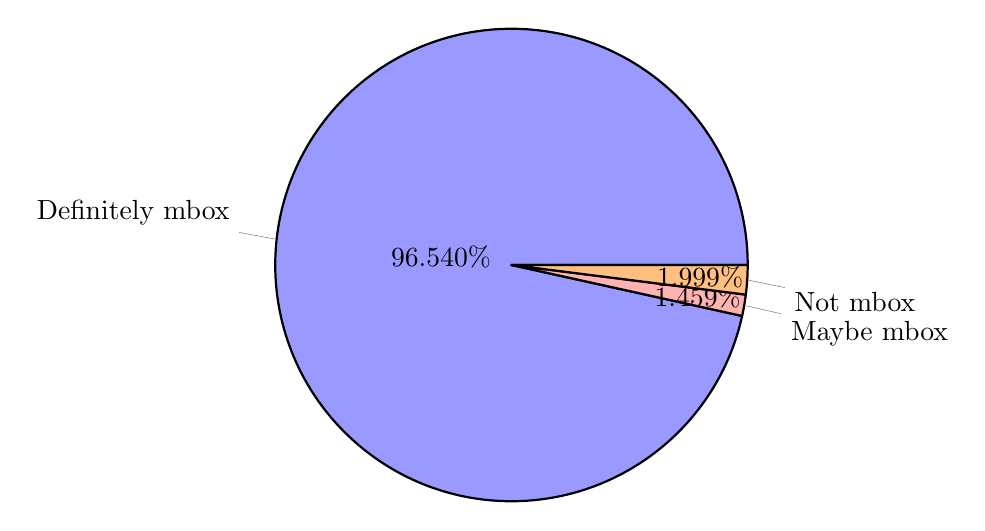
\begin{tikzpicture}   
  
\pie[ text=pin, color={blue!40, red!30, orange!50}]  
 {96.540/Definitely mbox, 1.459/Maybe mbox, 1.999/Not mbox}  
   

\end{tikzpicture}  
\caption{Categorization of downloaded mbox data.} \label{fig:f1}
\end{figure}




96.54\% of the data are categorized as 'definitely mbox' (approximately 2.9 GB), and 1.46\% and 1.99\% are in the 'maybe mbox' and 'not mbox' categories, respectively. A break-down of these numbers is shown in Figure \ref{fig:f1}

In order to determine the quality of files in category 2, two fresh Solr cores were created. Both of these cores use the exact same schema as the cores that hold files from category 1.
The raw unprocessed files were parsed and uploaded to test core 1, while the files processed by the cleanarch script were parsed and uploaded to test core 2.



\subsection{Choosing a starting point}

Before statistics based on time can be calculated, a concrete point in time has to be chosen as the beginning. This is no easy task, as there are many messages with fake or incorrect dates. The earliest date cannot be set to any earlier than the default value chosen for the date field, which is first of January 1900.

One way of solving this problem is to simply set the starting point to the date on which the IETF was founded, that date being 16. January 1982. It is safe to assume that since the organization did not exist, there was no one to keep track of the messages and archive them. It is however still possible that there was some communication regarding the organization prior to this date, for this reason, the default date for all statistics has been set to first of January 1980.

In fact, by using that date as a starting point, a grand total of 13348 (0.00461\% of the database) messages are lost, most of which seem to be either broken, incorrectly formatted, or simply spam.

These messages can be found by executing the following query in Solr:\\\\
\noindent
\textbf{Date:[0000-01-01T00:00:00Z TO 0000-01-01T00:00:00Z+1980YEAR]}  \\

These messages are still included in the statistics, they are however bundled in a “pre 1980” category, and will not be calculated on a year by year basis.\\\\


\section{Error report}
With the error definitions in place, these are the results:\\\\

\begin{figure}[H]
\begin{tikzpicture}
  \tikzset{venn circle/.style={draw,circle,minimum width=6cm,fill=#1,opacity=0.6}}

  \node [venn circle = white,text opacity=1] (A) at (0,0) {Date = 12736};
  \node [venn circle = white,text opacity=1] (B) at (60:4.5cm) {From = 89};
  \node [venn circle = white,text opacity=1] (C) at (0:4.5cm) {Dest = 18820};
  \node[left] at (barycentric cs:A=1/2,B=1/2 ) {29}; 
  \node[below] at (barycentric cs:A=1/2,C=1/2 ) {44};   
  \node[right] at (barycentric cs:B=1/2,C=1/2 ) {157};   
  \node[below] at (barycentric cs:A=1/3,B=1/3,C=1/3 ){6934};
\end{tikzpicture}
\caption{Distribution of errors across messages obtained from the raw files found in the IETF email archives. Each type of error is represented by a circle, the overlapping areas represent messages with the respective combination of errors.}
\end {figure}

There are 38 809 erroneous messages in total, and they make up 1.3322\% of the entire database.\\\\


\begin{center}
\begin{table}[H]
\begin{tabular}{||p{1.2cm}|p{1.2cm}|p{1.7cm}|p{1.5cm}|p{1.5cm}| p{2.5cm} ||} 
 \hline
 Year & From error & Destination error & Both & Total messages per year& Percent per year\\ [1ex] 
 \hline\hline
1980 & 0 & 0 & 0 & 43 & 0.000000\%\\
\hline
1981 & 0 & 0 & 0 & 1 & 0.000000\%\\
\hline
1982 & 0 & 0 & 0 & 0 & 0.000000\%\\
\hline
1983 & 0 & 0 & 0 & 0 & 0.000000\%\\
\hline
1984 & 0 & 0 & 0 & 1 & 0.000000\%\\
\hline
1985 & 0 & 0 & 0 & 1 & 0.000000\%\\
\hline
1986 & 0 & 0 & 0 & 0 & 0.000000\%\\
\hline
1987 & 0 & 0 & 0 & 16 & 0.000000\%\\
\hline
1988 & 0 & 0 & 0 & 25 & 0.000000\%\\
\hline
1989 & 0 & 0 & 0 & 1 & 0.000000\%\\
\hline
1990 & 0 & 0 & 0 & 14 & 0.000000\%\\
\hline
1991 & 0 & 0 & 0 & 2 & 0.000000\%\\
\hline
1992 & 0 & 0 & 0 & 7 & 0.000000\%\\
\hline
1993 & 0 & 0 & 0 & 76 & 0.000000\%\\
\hline
1994 & 0 & 0 & 0 & 46 & 0.000000\%\\
\hline
1995 & 0 & 3 & 0 & 125 & 2.400000\%\\
\hline
1996 & 2 & 3 & 0 & 390 & 1.282051\%\\
\hline
1997 & 0 & 8 & 0 & 6794 & 0.117751\%\\
\hline
1998 & 0 & 63 & 0 & 32945 & 0.191228\%\\
\hline
1999 & 0 & 217 & 4 & 47930 & 0.461089\%\\
\hline
2000 & 1 & 360 & 3 & 61694 & 0.590009\%\\
\hline
2001 & 3 & 276 & 0 & 103630 & 0.269227\%\\
\hline
2002 & 37 & 1175 & 11 & 124445 & 0.982763\%\\
\hline
2003 & 11 & 2319 & 6 & 139301 & 1.676944\%\\
\hline
2004 & 9 & 2863 & 75 & 120907 & 2.437411\%\\
\hline
2005 & 9 & 3774 & 1 & 138451 & 2.733097\%\\
\hline
2006 & 1 & 4450 & 16 & 138231 & 3.231547\%\\
\hline
2007 & 3 & 2728 & 15 & 211617 & 1.297627\%\\
\hline
2008 & 5 & 47 & 1 & 146306 & 0.036225\%\\
\hline
2009 & 0 & 22 & 0 & 170228 & 0.012924\%\\
\hline
2010 & 0 & 41 & 0 & 163604 & 0.025061\%\\
\hline
2011 & 0 & 230 & 18 & 129324 & 0.191766\%\\
\hline
2012 & 0 & 76 & 0 & 122797 & 0.061891\%\\
\hline
2013 & 0 & 17 & 0 & 132088 & 0.012870\%\\
\hline
2014 & 6 & 30 & 2 & 146231 & 0.025986\%\\
\hline
2015 & 2 & 16 & 0 & 133848 & 0.013448\%\\
\hline
2016 & 0 & 28 & 3 & 118598 & 0.026139\%\\
\hline
2017 & 0 & 43 & 0 & 130735 & 0.032891\%\\
\hline
2018 & 0 & 11 & 2 & 136456 & 0.009527\%\\
\hline
2019 & 0 & 5 & 0 & 126353 & 0.003957\%\\
\hline
2020 & 0 & 10 & 0 & 109885 & 0.009100\%\\
\hline

\end{tabular}
\caption{Error rate over time.}
\end{table}
\end{center}


\subsection{The effects of Cleanarch}

As previously  described, cleanarch is a script developed by the IETF to correct the shortcoming of the mbox format. By simply using two Solr cores, one containing the parse of the clean data, and the other containing the raw data the effects of cleanarch can be clearly observed. 
The modified cleanarch script also outputs a new clean file for every .mail file in any subdirectory, meaning it is also possible to observe the effects Cleanarch has on the file size, even if this difference is not expected to be major.\\

\noindent
Like expected the difference is negligible: \\
\noindent

\begin{center}
\begin{tabular}{||p{2cm}|p{2cm}||} 
\hline
Category & Count\\

\hline
mail  bytes  & 29107339665\\
\hline
mailcl bytes & 29107362679\\
\hline

\end{tabular}
\end{center}




The difference is 0,023 megabytes.\\\\
\noindent
The post parse difference however, is greater.\\




\begin{center}
\begin{tabular}{||p{2cm}|p{5cm}||} 
\hline
Type of files & Solr document count\\

\hline
Clean   & 2893656\\
\hline
Default & 2913059\\
\hline

\end{tabular}
\end{center}






The clean archives produce 2893656 Solr documents \\
The default archives produce 2913059 Solr documents.\\
The difference is 19403 documents.\\\\



\begin{figure}[H]
\begin{tikzpicture}
  \tikzset{venn circle/.style={draw,circle,minimum width=6cm,fill=#1,opacity=0.6}}

  \node [venn circle = white,text opacity=1] (A) at (0,0) {Date = 12736};
  \node [venn circle = white,text opacity=1] (B) at (60:4.5cm) {From = 89};
  \node [venn circle = white,text opacity=1] (C) at (0:4.5cm) {Dest = 7501};
  \node[left] at (barycentric cs:A=1/2,B=1/2 ) {22}; 
  \node[below] at (barycentric cs:A=1/2,C=1/2 ) {44};   
  \node[right] at (barycentric cs:B=1/2,C=1/2 ) {157};   
  \node[below] at (barycentric cs:A=1/3,B=1/3,C=1/3 ){443};
\end{tikzpicture}
\caption{Distribution of errors across messages obtained from the clean files produced by the cleanarch program.  Each type of error is represented by a circle, the overlapping areas represent messages with the respective combination of errors.}
\end {figure}


There are 20 992 erroneous messages in total, and they make up 0.725\% of the entire database.\\\\
We can see that CleanArch successfully eliminates 54\% of all errors, mostly in messages that have all 3 types of errors simultaneously. 


\subsection{A closer look at category 2}

As previously mentioned not all files in the IETF email archive carry the “.mail” extension. This does not mean that unmarked mbox files do not exist, as we saw previously. 
When parsed, these unmarked files produce a total of 107136 Solr documents.\\

The biggest difference between category 1 and 2 is the error rate. When looking at filenames of category 2 it is quite common to see the “.broken” file extension, implying these files were excluded from the rest for a reason.

This does not mean that these files are useless however, because as long as there is some context to a message, it still holds value. Recall chapter 5, in the parsing process, some of the information is extracted from the filename,thus there will always be some fields with information.
This also means that as long as the directory structure of the archive is consistent, at the very least the mailing list of a message will always be known.
However, the directory structure is not always consistent. For all category 1 files, the leaf node folder has the name of the mailing list. This means that it is safe to simply split the directory string and use the last item in the resulting list as the mailing list name.

The unmarked files do not always follow this structure, and in some cases they are contained in yet another subfolder.
For this reason a small change to the parser had to be done; it now uses the n-th position in the split directory string as the mailing list, instead of using the last.\\

The error analysis of category 2 files returns the following results:\\\\
\noindent


\begin{center}

 \begin{tabular}{|c | c|}
 \hline
 Error combination & Value \\ [0.5ex]
 \hline\hline
ALL & 11219\\
\hline
From + Date + Dest & 7297\\
\hline
From + Date & 13\\
\hline
From + Dest & 0\\
\hline
Date + Dest & 2\\
\hline
From & 12\\
\hline
Date & 93\\
\hline
Dest & 3802\\
\hline

\end{tabular}
\captionof{table}{Distribution of errors in files from category 2.}
\end{center}



The 5 largest sources of errors in category 2 are the following mailing lists: \\\\
\noindent
\begin{center}
 \begin{tabular}{|c | c|}
 \hline
Error combination & Value \\ [0.5ex]
 \hline\hline
All & 7150\\
\hline
From + Date + Dest & 7065\\
\hline
From + Date & 1\\
\hline
From + Dest & 0\\
\hline
Date + Dest & 1\\
\hline
From & 2\\
\hline
Date & 10\\
\hline
Dest & 71\\
\hline
\end{tabular}
\captionof{table}{Stats for mailing list avt.}
\end{center}

\bigskip

\begin{center}
 \begin{tabular}{|c | c|}
 \hline
Error combination & Value \\ [0.5ex]
 \hline\hline
All & 2529\\
\hline
From + Date + Dest & 0\\
\hline
From + Date & 0\\
\hline
From + Dest & 0\\
\hline
Date + Dest & 0\\
\hline
From & 0\\
\hline
Date & 0\\
\hline
Dest & 2529\\
\hline
\end{tabular}
\captionof{table}{Stats for mailing list isis-wg}
\end{center}


\bigskip

\begin{center}
 \begin{tabular}{|c | c|}
 \hline
Error combination & Value \\ [0.5ex]
 \hline\hline
All & 756\\
\hline
From + Date + Dest & 9\\
\hline
From + Date & 0\\
\hline
From + Dest & 0\\
\hline
Date + Dest & 0\\
\hline
From & 0\\
\hline
Date & 0\\
\hline
Dest & 747\\
\hline
\end{tabular}
\captionof{table}{Stats for mailing list capwap.}
\end{center}



\bigskip


\begin{center}
 \begin{tabular}{|c | c|}
 \hline
Error combination & Value \\ [0.5ex]
 \hline\hline
All & 293\\
\hline
From + Date + Dest & 0\\
\hline
From + Date & 0\\
\hline
From + Dest & 0\\
\hline
Date + Dest & 0\\
\hline
From & 0\\
\hline
Date & 0\\
\hline
Dest & 293\\
\hline
\end{tabular}
\captionof{table}{Stats for mailing list tap.}
\end{center}

\bigskip

\begin{figure}[H]
\begin{center}
 \begin{tabular}{|c | c|}
 \hline
Error combination & Value \\ [0.5ex]
 \hline\hline
All & 165\\
\hline
From + Date + Dest & 130\\
\hline
From + Date & 0\\
\hline
From + Dest & 0\\
\hline
Date + Dest & 0\\
\hline
From & 9\\
\hline
Date & 26\\
\hline
Dest & 0\\
\hline
\end{tabular}
\captionof{table}{Stats for mailing list i-d-announce.}
\end{center}
\end{figure}

These 5 mailing lists are responsible for 97\% of all errors in category 2 files. The remaining mailing lists contain between 0 to 3 errors each, for the full results please see the github repository.



\subsection{Cleaning category 2 }

As with category 1 the cleanarch script was used to try and fix errors in the mbox files.
The results were quite different from category 1. The most significant difference is the decrease in documents count. As the purpose of cleanarch is to fix incorrectly separated messages in a mbox file, the expectation is that the amount of documents should increase, not decrease.\\

The raw files generate 107136 files after parsing.
The clean files generate 106030 files, which is 1106 fewer.
\noindent
The error analysis tells a similar story:\\\\

\begin{center}
 \begin{tabular}{|c | c|}
 \hline
 Category & Value \\ [0.5ex]
 \hline\hline
From + Date + Dest & 7193\\
\hline
From + Date & 13\\
\hline
From + Dest & 0\\
\hline
Date + Dest & 2\\
\hline
From & 11\\
\hline
Date & 93\\
\hline
Dest & 2811\\
\hline
ALL & 10123\\
\hline
\end{tabular}
\captionof{table}{Distribution of errors in clean files from category 2.}
\end{center}


As we can see the error count has dropped by 1106, which is very close to the total decrease in document count, which is 1096.
This could mean that instead of fixing boundaries between messages, it actually does the opposite.\\

\noindent
The average length of the “Content” field in the raw files is 2479.721.
\noindent
The same average for the clean files is 2483.450
\noindent
Which confirms that cleanarch does indeed make messages longer in this case.\\


\subsection{Error rate over time }

The error rate over time in category 2 raw files is as follows:\\
(Only years with errors are shown)\\\\

\begin{center}
 \begin{tabular}{|c | c|}
 \hline
Year& Error count \\ [0.5ex]
 \hline\hline
 1993 & 1\\
\hline
1994 & 1\\
\hline
1995 & 1\\
\hline
2006 & 9\\
\hline


\end{tabular}
\captionof{table}{Errors in the "From" field found in the raw category 2 files.}
\end{center}

\begin{figure}[H]
\centering
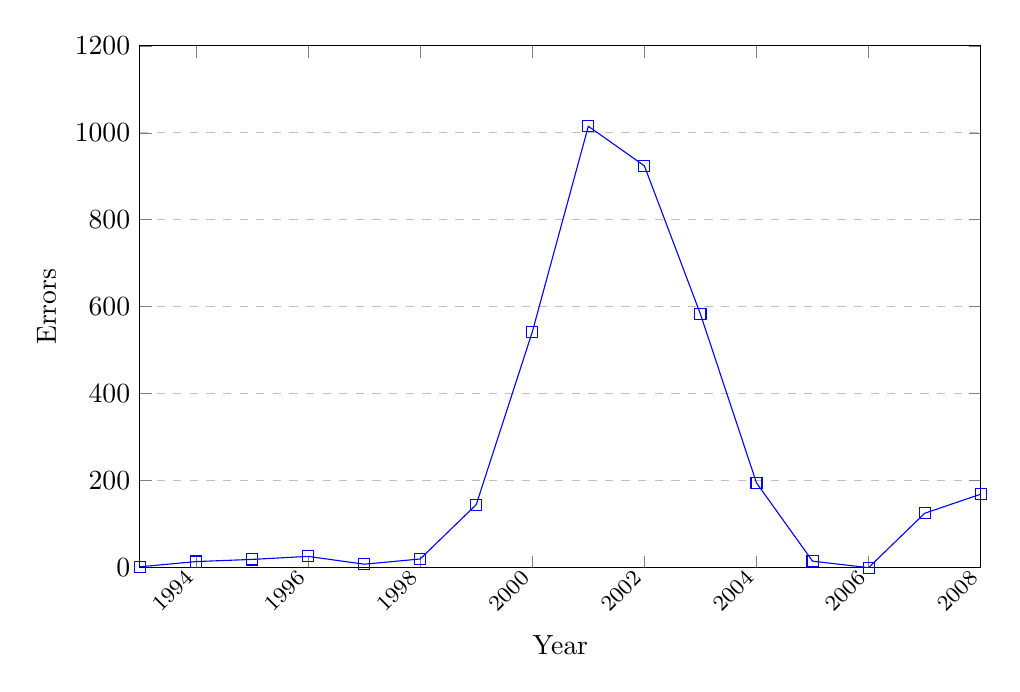
\begin{tikzpicture}
\begin{axis}[
     /pgf/number format/.cd,
     use comma,
    1000 sep={},
    width=8.7cm, height=6cm, 
    xlabel={Year},
    ylabel={Errors},
    scale=1.5,
    xmin=1993, xmax=2008,
    ymin=0, ymax=1200,
    x tick label style={font=\footnotesize,rotate=45, anchor=east},
    legend pos=north west,
    ymajorgrids=true,
    grid style=dashed,
]
\addplot[
    color=blue,
    mark=square,
    ]
    coordinates {(1993,2)(1994,14)(1995,19)(1996,26)(1997,8)(1998,20)(1999,145)(2000,542)(2001,1015)(2002,924)(2003,583)(2004,195)(2005,15)(2006,0)(2007,125)(2008,169)};
  
    
\end{axis}
\end{tikzpicture}
\caption{Destination errors per year}
\end{figure}


The results show errors from the years they first appeared to the last years they appeared. It is also important to remember that these can only show errors in messages that do not also have an error in their date field. As just the “avt” mailing list has 7076 messages with date errors, the amount of messages depicted in these tables is significantly smaller than the total amount of messages with errors.\\


In conclusion, category 2 files have a much larger frequency of errors than their category 1 counterparts. Those errors however are concentrated in just 5 out of 118 mailing lists found in these files. 
For this reason it was decided that adding these files to the main Solr core would still be beneficial to this project. 
All statistics from this point on will be calculated using a core containing clean files from both category 1 and 2.


\section{Final error rate}


The final error rate in the  core used for calculating statistics from this point in is depicted in the figure \ref{fig:fe}. 

\begin{figure}[H]
\begin{tikzpicture}
  \tikzset{venn circle/.style={draw,circle,minimum width=6cm,fill=#1,opacity=0.6}}

  \node [venn circle = white,text opacity=100] (A) at (0,0) {Date = 12829};
  \node [venn circle = white,text opacity=100] (B) at (60:4.5cm) {From = 100};
  \node [venn circle = white,text opacity=100] (C) at (0:4.5cm) {Dest = 10312};
  \node[left] at (barycentric cs:A=1/2,B=1/2 ) {35}; 
  \node[below] at (barycentric cs:A=1/2,C=1/2 ) {46};   
  \node[right] at (barycentric cs:B=1/2,C=1/2 ) {157};   
  \node[below] at (barycentric cs:A=1/3,B=1/3,C=1/3 ){7636};
\end{tikzpicture}\\\\

\caption{Error rate in the main and final Solr core.}

\label{fig:fe}

\end{figure}


\subsection{Implementing some aggregation functions}


Like mentioned Solr does not support sql functions like min(), max(). This is not entirely correct however, Solr has support for these functions, they can be used on the various fields in the documents. 
For example\\ 

max(field1,field2)\\

However, they cannot be used on the results returned by a facet field query. For this reason more general versions of these functions have been implemented to streamline the calculation of statistics.
All of the functions below take a Solr object as the first arguments, so a connection has to be established before these functions can be used.
The following methods have been implemented:\\



max(solr,field)\\

min(solr,field)\\

avg(solr,field)\\

unique(solr,field)\\


\section{General statistics}


\begin{figure}[H]
\hspace*{-0.3cm}
\centering
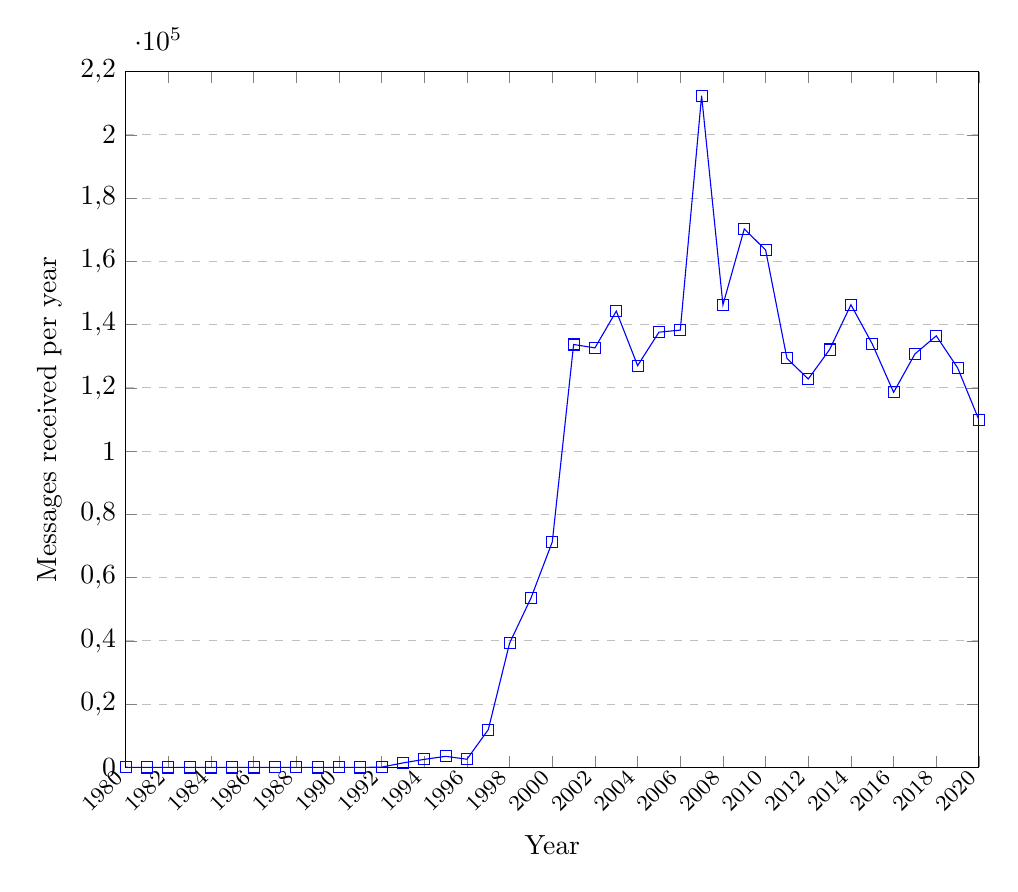
\begin{tikzpicture}
\begin{axis}[
     /pgf/number format/.cd,
     use comma,
    1000 sep={},
    width=7cm, height=6cm, 
    xlabel={Year},
    ylabel={Messages received per year},
    scale=2,
    xmin=1980, xmax=2020,
    ymin=0, ymax=220000,
    xtick={1980,1982,1984,1986,1988,1990,1992 ,1994,1996,1998,2000,2002,2004,2006,2008,2010,2012,2014,2016,2018,2020},
    x tick label style={font=\footnotesize,rotate=45, anchor=east},
    legend pos=north west,
    ymajorgrids=true,
    grid style=dashed,
]
\addplot[
    color=blue,
    mark=square,
    ]
    coordinates {(1980,44)(1981,1)(1982,0)(1983,0)(1984,1)(1985,1)(1986,0)(1987,17)(1988,25)(1989,2)(1990,14)(1991,2)(1992,90)(1993,1429)(1994,2548)(1995,3513)(1996,2586)(1997,11951)(1998,39318)(1999,53552)(2000,71311)(2001,133723)(2002,132650)(2003,144272)(2004,127047)(2005,137615)(2006,138269)(2007,212367)(2008,146271)(2009,170249)(2010,163604)(2011,129325)(2012,122814)(2013,132127)(2014,146299)(2015,133892)(2016,118598)(2017,130735)(2018,136456)(2019,126353)(2020,109885)

    };
 
    
\end{axis}
\end{tikzpicture}
\caption{Messages were sent per year.} \label{fig:mpy}
\end{figure}


As we can see in figure \ref{fig:mpy}, there are close to no messages sent between the years 1980 and 1990. This may be due to the archival system not being as well developed as it is today, resulting in a major loss of data. Another possibility is that email was not as widely used as it is today. During this period communication media like fax, phone calls, and paper mail were more commonly used.
Since this decade is essentially devoid of data, the earliest year included from this point on is 1990.






\subsection{Top 20 contributors}

\begin{center}
 \begin{tabular}{|c | c | c|}
 \hline
Ranking & address & Value \\ [0.5ex]
 \hline\hline
 1 & internet-drafts@ietf.org & 190901\\
  \hline
 2 & notifications@github.com & 41934\\
  \hline
 3 & iesg-secretary@ietf.org & 27170\\
  \hline
 4 & black\_david@emc.com & 14365\\
  \hline
 5 & rfc-editor@rfc-editor.org & 14198\\
  \hline
 6 & brian.e.carpenter@gmail.com & 13491\\
  \hline
 7 & marcelrf@bellsouth.net & 11485\\
  \hline
 8 & julian.reschke@gmx.de & 10500\\
  \hline
 9 & christer.holmberg@ericsson.com & 10230\\
  \hline
 10 & noreply@github.com & 8953\\
  \hline
 11 & stephen.farrell@cs.tcd.ie & 8567\\
  \hline
 12 & martin.thomson@gmail.com & 8522\\
  \hline
 13 & cabo@tzi.org & 7915\\
  \hline
 14 & dromasca@avaya.com & 7606\\
  \hline
 15 & jari.arkko@piuha.net & 7482\\
  \hline
 16 & j.schoenwaelder@jacobs-university.de & 7306\\
  \hline
 17 & feedback@oneoffice.jp & 7194\\
  \hline
 18 & paul.hoffman@vpnc.org & 7108\\
  \hline
 19 & mcr+ietf@sandelman.ca & 7101\\
  \hline
 20 & mnot@mnot.net & 7043\\
  \hline
\end{tabular}
\captionof{table}{Top 20 posters.}
\end{center}

As we can see in the graph and table above, there are some email addresses that do not seem to belong to any one individual, instead their names imply that they are automatically generated messages. There is no surefire way to know which messages exactly come from some form of automatic messaging system, it is however possible to make an educated guess. For this reason, a blacklist of addresses that are believed to not belong to individuals and found in the top fifty most active addresses, has been created in order to improve the quality of the data displayed. This blacklist was manually created by the author with help from Michael Welzl..\\


The blacklist contains the following addresses: 

\begin{itemize}
\item internet-drafts@ietf.org
\item notifications@github.com
\item noreply@github.com
\item iesg-secretary@ietf.org
\item ietf-secretariat-reply@ietf.org
\item rfc-editor@rfc-editor.org
\item noreply@ietf.org
\item trac@tools.ietf.org
\item feedback@oneoffice.jp


\end{itemize}

With these addresses excluded, the top 20 table looks quite different: 

\begin{center}
 \begin{tabular}{|c | c | c|}
 \hline
Ranking & address & Value \\ [0.5ex]
 \hline\hline
 1 & black\_david@emc.com & 14365\\
  \hline
 2 & brian.e.carpenter@gmail.com & 13491\\
  \hline
 3 & marcelrf@bellsouth.net & 11485\\
  \hline
 4 & julian.reschke@gmx.de & 10500\\
  \hline
 5 & christer.holmberg@ericsson.com & 10230\\
  \hline
 6 & stephen.farrell@cs.tcd.ie & 8567\\
  \hline
 7 & martin.thomson@gmail.com & 8522\\
  \hline
 8 & cabo@tzi.org & 7915\\
  \hline
 9 & dromasca@avaya.com & 7606\\
  \hline
 10 & jari.arkko@piuha.net & 7482\\
  \hline
 11 & j.schoenwaelder@jacobs-university.de & 7306\\
  \hline
 12 & paul.hoffman@vpnc.org & 7108\\
  \hline
 13 & mcr+ietf@sandelman.ca & 7101\\
  \hline
 14 & mnot@mnot.net & 7043\\
  \hline
 15 & adrian@olddog.co.uk & 6811\\
  \hline
 16 & randy@psg.com & 6316\\
  \hline
 17 & ekr@rtfm.com & 6135\\
  \hline
 18 & john-ietf@jck.com & 5979\\
  \hline
 19 & housley@vigilsec.com & 5910\\
  \hline
 20 & fred@cisco.com & 5857\\
  \hline
\end{tabular}
\captionof{table}{Top 20 posters, after filtering out the blacklisted addresses.}
\end{center}

From this point on, the graphs and tables in this thesis will have these addresses excluded from them, unless explicitly stated otherwise.

\subsection{Top 10 mailing lists}


\begin{center}
 \begin{tabular}{|c | c | c|}
 \hline
Ranking & address & Value \\ [0.5ex]
 \hline\hline
1 & ietf & 134157\\
\hline
2 & i-d-announce & 103544\\
\hline
3 & quic-issues & 54104\\
\hline
4 & v6ops & 44450\\
\hline
5 & ips & 40603\\
\hline
6 & avt & 40454\\
\hline
7 & dmarc-report & 40007\\
\hline
8 & ipv6 & 38591\\
\hline
9 & httpbisa & 38133\\
\hline
10 & mobileip & 37475\\
\hline
\end{tabular}

\captionof{table}{Most active mailing  lists, measured by the total amount of messages sent.}

\end{center}



\subsection{Top mailing list per year}




\begin{center}
 \begin{tabular}{|c | c | c|}
 \hline
 Year & Mailing-list & Count \\ [0.5ex]
 \hline\hline
1990 & webdav & 3\\
\hline
1991 & idn & 1\\
\hline
1992 & ipsec & 78\\
\hline
1993 & avt & 1067\\
\hline
1994 & avt & 1650\\
\hline
1995 & ipsec & 1638\\
\hline
1996 & avt & 1540\\
\hline
1997 & ietf & 2574\\
\hline
1998 & ietf & 13383\\
\hline
1999 & ietf-announce-old & 7177\\
\hline
2000 & sip & 5739\\
\hline
2001 & ips & 25894\\
\hline
2002 & mobileip & 7591\\
\hline
2003 & mobileip & 15731\\
\hline
2004 & marid & 8742\\
\hline
2005 & ietf & 6271\\
\hline
2006 & i-d-announce & 7151\\
\hline
2007 & ietf & 6313\\
\hline
2008 & i-d-announce & 5072\\
\hline
2009 & i-d-announce & 5428\\
\hline
2010 & i-d-announce & 6342\\
\hline
2011 & i-d-announce & 6477\\
\hline
2012 & i-d-announce & 6985\\
\hline
2013 & ietf & 8614\\
\hline
2014 & i-d-announce & 7148\\
\hline
2015 & i-d-announce & 7044\\
\hline
2016 & i-d-announce & 6696\\
\hline
2017 & quic-issues & 9143\\
\hline
2018 & dmarc-report & 16635\\
\hline
2019 & quic-issues & 15433\\
\hline
2020 & quic-issues & 14328\\
\hline
\end{tabular}

\captionof{table}{Most active mailing list per year, measured by the total amount of messages sent per year.}
\end{center}



















\section{Crosstalk}

In order to gain a better understanding of how working in the IETF is done, it is important to understand how working groups and people interact with each other.
There are many ways of defining what an interaction, in the context of this project, is.
For this reason several options have been defined and explored.\\

\noindent
\textbf{Definition 1} \\

\textit{An interaction is defined as the act of sending a message to a mailing list, performed by any entity.}\\

This definition essentially says that if an address appears in the “From” field, it is considered an interaction from an entity identified by the address found in this field.

The simplest way of checking how many mailing lists an entity has interacted with  is checking how many different mailing lists an email address appears in. 

While this method does not give any specifics regarding groups or people, it sheds some light on the average crossinteraction per email address, whomever that address may belong to. The database also makes it possible to see how this has developed over time.

\subsection{The results}

Based on all unique values found in the “From-address” field, each value appears on average in 1.52 mailing lists.
The following graph shows how this developed over time.


\begin{figure}[H]
\hspace*{-0.3cm}
\centering
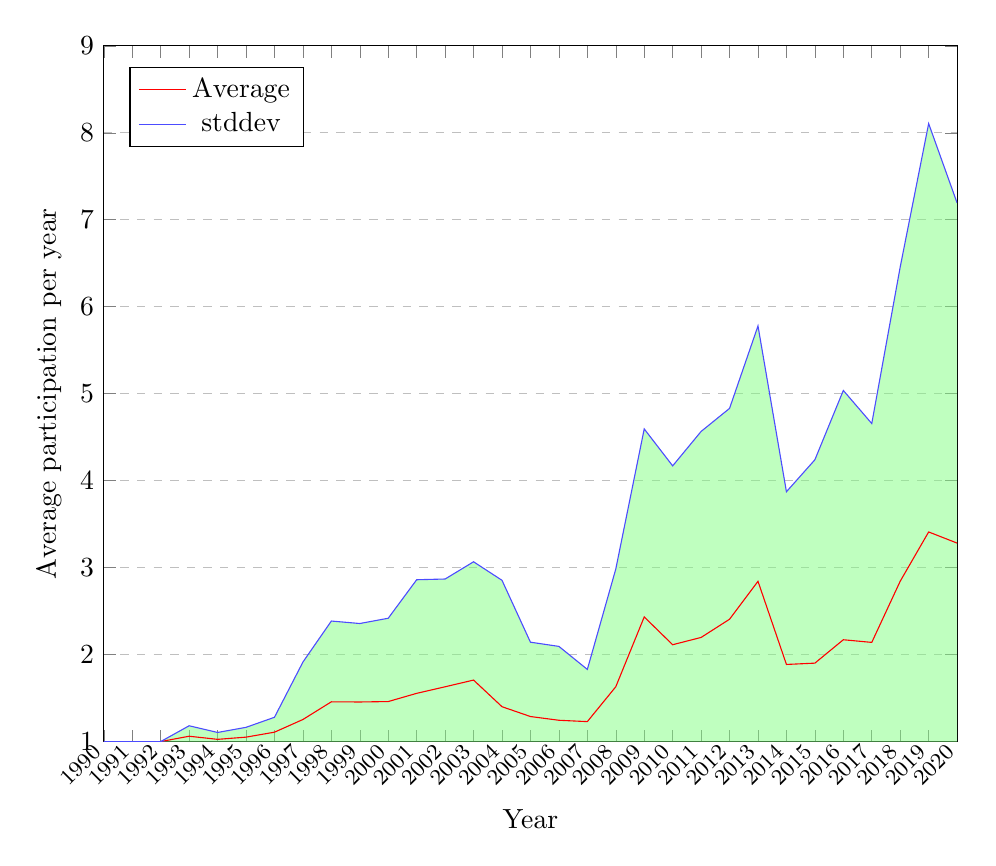
\begin{tikzpicture}
\begin{axis}[
     /pgf/number format/.cd,
     use comma,
    1000 sep={},
    width=7cm, height=6cm, 
    xlabel={Year},
    ylabel={Average participation per year},
    scale=2,
    xmin=1990, xmax=2020,
    ymin=1, ymax=9,
    xtick={1990,1991,1992,1993 ,1994,1995,1996,1997,1998,1999,2000,2001,2002,2003,2004,2005,2006,2007,2008,2009,2010,2011,2012,2013,2014,2015,2016,2017,2018,2019,2020},
    x tick label style={font=\footnotesize,rotate=45, anchor=east},
    ytick={-2,-1,0,1,2,3,4,5,6,7,8,9},
    legend pos=north west,
    ymajorgrids=true,
    grid style=dashed,
]
\addplot[color=red] coordinates {
(1990,1.0)(1991,1.0)(1992,1.0)(1993,1.061611374407583)(1994,1.025706940874036)(1995,1.0511363636363635)(1996,1.1080368906455862)(1997,1.2538825118163404)(1998,1.4574123989218328)(1999,1.4553291536050157)(2000,1.460261353898886)(2001,1.5546861106171084)(2002,1.630135712957799)(2003,1.7072126468328028)(2004,1.4009501187648457)(2005,1.288095490341491)(2006,1.245071905749169)(2007,1.2295182766516835)(2008,1.6303503907234687)(2009,2.4331026528258364)(2010,2.1137116361227646)(2011,2.1974873781848068)(2012,2.4067170175156676)(2013,2.842758620689655)(2014,1.8868374032162)(2015,1.9019427231619495)(2016,2.170932561762742)(2017,2.1404308572450166)(2018,2.843798449612403)(2019,3.4104060913705583)(2020,3.2822724568709103)};

\addplot[name path=us_top,color=blue!70] coordinates {
(1990,1.0)(1991,1.0)(1992,1.0)(1993,1.1818355534973064)(1994,1.1048367299312154)(1995,1.1638241660188091)(1996,1.279388349504036)(1997,1.913888365681723)(1998,2.386094737898442)(1999,2.357613541329531)(2000,2.418153427001008)(2001,2.860937479349478)(2002,2.869191821083624)(2003,3.067274301985157)(2004,2.85433702648582)(2005,2.1428371873223417)(2006,2.094459579000438)(2007,1.8297360261982423)(2008,2.983495757256312)(2009,4.594975396148838)(2010,4.170163209301785)(2011,4.56597141493077)(2012,4.831146086059229)(2013,5.779233178142352)(2014,3.8726697834032557)(2015,4.240196249591621)(2016,5.03732574318372)(2017,4.656857551129747)(2018,6.457015074372294)(2019,8.10575272766)(2020,7.193648688742229)};

\addplot[name path=us_down,color=blue!70] coordinates {
(1990,1.0)(1991,1.0)(1992,1.0)(1993,0.9413871953178596)(1994,0.9465771518168566)(1995,0.9384485612539178)(1996,0.9366854317871366)(1997,0.5938766579509578)(1998,0.5287300599452239)(1999,0.5530447658805)(2000,0.502369280796764)(2001,0.24843474188473857)(2002,0.39107960483197357)(2003,0.3471509916804485)(2004,-0.052436788956128355)(2005,0.43335379336063995)(2006,0.3956842324979001)(2007,0.6293005271051245)(2008,0.2772050241906254)(2009,0.2712299095028343)(2010,0.05726006294374386)(2011,-0.17099665856115642)(2012,-0.017712051027893416)(2013,-0.0937159367630418)(2014,-0.09899497697085557)(2015,-0.43631080326772276)(2016,-0.6954606196582351)(2017,-0.37599583663971314)(2018,-0.7694181751474884)(2019,-1.284940544918884)(2020,-0.6291037750004089)};

\addplot[green!50,fill opacity=0.5] fill between[of=us_top and us_down];


 \legend{Average, stddev}

  
    
\end{axis}
\end{tikzpicture}
\caption{The number of mailing lists an email address appears in, per year.}
\end{figure}



How is this distributed?
Figure \ref{fig:apy} shows how many entities are participating in how many working groups, and figure \ref{fig:apyc} plots the same data in the form of a Cumulative Distribution Function (CDF).\\\\

\begin{figure}[H]

\centering
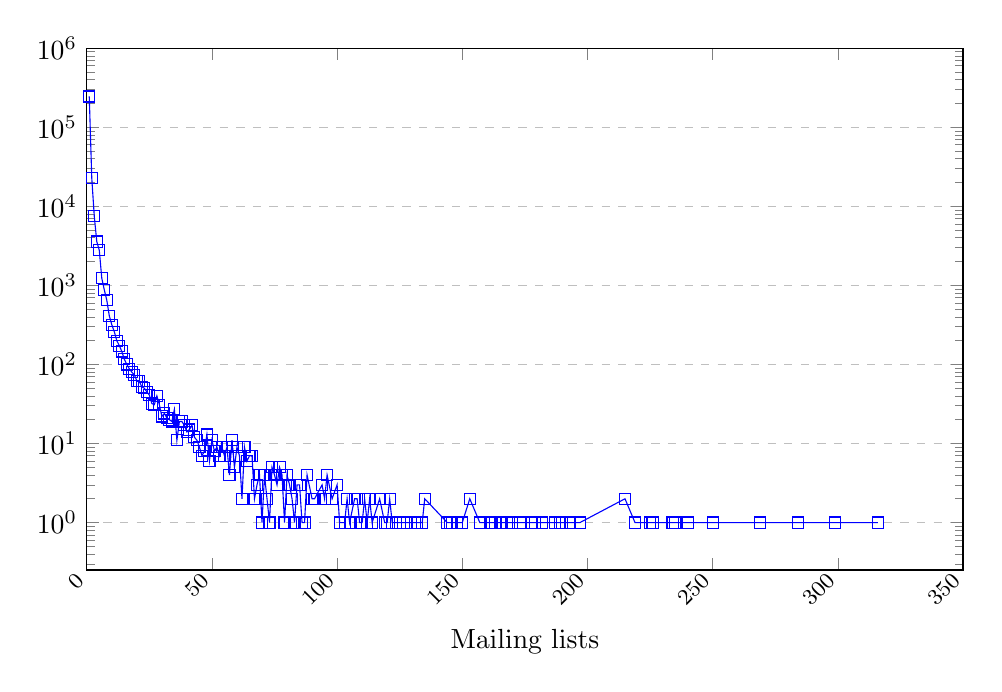
\begin{tikzpicture}
\begin{axis}[
     /pgf/number format/.cd,
     use comma,
    1000 sep={},
    width=9cm, height=6cm, 
    xlabel={Mailing lists},
    scale=1.5,
    xmin=0, xmax=350,
    ymode=log,
    ymin=0, ymax=1e6,
    x tick label style={font=\footnotesize,rotate=45, anchor=east},
    legend pos=north west,
    ymajorgrids=true,
    grid style=dashed,
]
\addplot[
    color=blue,
    mark=square,
    ]
    coordinates {
(1.0,244788)(2.0,22764)(3.0,7489)(4.0,3579)(5.0,2778)(6.0,1233)(7.0,878)(8.0,649)(9.0,412)(10.0,318)(11.0,259)(12.0,200)(13.0,173)(14.0,146)(15.0,116)(16.0,100)(17.0,88)(18.0,80)(19.0,74)(20.0,62)(21.0,61)(22.0,52)(23.0,50)(24.0,45)(25.0,41)(26.0,32)(27.0,31)(28.0,40)(29.0,31)(30.0,22)(31.0,24)(32.0,21)(33.0,20)(34.0,19)(35.0,27)(36.0,11)(37.0,19)(38.0,19)(39.0,17)(40.0,14)(41.0,15)(42.0,17)(43.0,12)(44.0,11)(45.0,9)(46.0,7)(47.0,8)(48.0,13)(49.0,6)(50.0,11)(51.0,8)(52.0,9)(53.0,7)(54.0,9)(55.0,7)(56.0,9)(57.0,4)(58.0,11)(59.0,5)(60.0,9)(61.0,7)(62.0,2)(63.0,9)(64.0,6)(65.0,7)(66.0,7)(67.0,2)(68.0,3)(69.0,4)(70.0,1)(71.0,4)(72.0,2)(73.0,1)(74.0,5)(75.0,4)(76.0,3)(77.0,5)(78.0,4)(79.0,1)(80.0,4)(81.0,3)(82.0,2)(83.0,1)(84.0,3)(85.0,3)(86.0,1)(87.0,1)(88.0,4)(90.0,2)(91.0,2)(94.0,3)(95.0,2)(96.0,4)(98.0,2)(100.0,3)(101.0,1)(103.0,1)(104.0,2)(105.0,1)(107.0,2)(108.0,2)(109.0,1)(110.0,1)(111.0,2)(112.0,1)(113.0,2)(114.0,1)(117.0,2)(119.0,1)(120.0,1)(121.0,2)(122.0,1)(125.0,1)(128.0,1)(131.0,1)(132.0,1)(134.0,1)(135.0,2)(144.0,1)(145.0,1)(146.0,1)(148.0,1)(150.0,1)(153.0,2)(157.0,1)(161.0,1)(162.0,1)(163.0,1)(165.0,1)(166.0,1)(168.0,1)(170.0,1)(173.0,1)(178.0,1)(179.0,1)(182.0,1)(187.0,1)(189.0,1)(190.0,1)(193.0,1)(197.0,1)(215.0,2)(219.0,1)(225.0,1)(226.0,1)(234.0,1)(235.0,1)(240.0,1)(250.0,1)(269.0,1)(284.0,1)(299.0,1)(316.0,1)

    };
  
    
\end{axis}
\end{tikzpicture}
\caption{The number of users sending messages to one or more multiple mailing lists.}  \label{fig:apy}
\end{figure}





\begin{figure}[H]

\centering
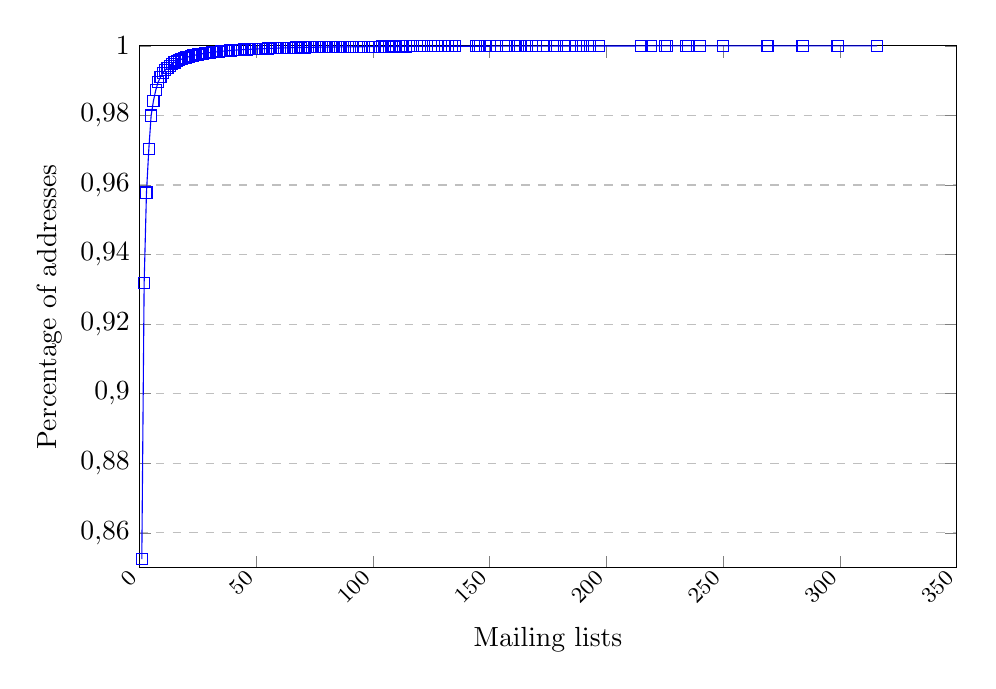
\begin{tikzpicture}
\begin{axis}[
     /pgf/number format/.cd,
     use comma,
    1000 sep={},
    width=8.5cm, height=6cm, 
    ylabel={Percentage of addresses},
    xlabel={Mailing lists},
    scale=1.5,
    xmin=0, xmax=350,
    ymin=0.85, ymax=1,
    x tick label style={font=\footnotesize,rotate=45, anchor=east},
    legend pos=north west,
    ymajorgrids=true,
    grid style=dashed,
]
\addplot[
    color=blue,
    mark=square,
    ]
    coordinates {
(1.0,0.8524624417559915)(2.0,0.9317369773710273)(3.0,0.9578170598354889)(4.0,0.9702807552741735)(5.0,0.9799550067211322)(6.0,0.9842488699443505)(7.0,0.9873064627342819)(8.0,0.9895665740334455)(9.0,0.9910013442264429)(10.0,0.9921087639385139)(11.0,0.9930107189870244)(12.0,0.9937072093719747)(13.0,0.9943096735549566)(14.0,0.9948181115359702)(15.0,0.9952220759592414)(16.0,0.9955703211517165)(17.0,0.9958767769210946)(18.0,0.9961553730750747)(19.0,0.9964130745175063)(20.0,0.9966289865368408)(21.0,0.9968414161042507)(22.0,0.9970225036043378)(23.0,0.9971966262005753)(24.0,0.997353336537189)(25.0,0.9974961170661039)(26.0,0.997607555527696)(27.0,0.9977155115373633)(28.0,0.9978548096143532)(29.0,0.9979627656240205)(30.0,0.9980393795663651)(31.0,0.9981229584125592)(32.0,0.9981960899029789)(33.0,0.998265738941474)(34.0,0.9983319055280442)(35.0,0.9984259317300125)(36.0,0.9984642387011847)(37.0,0.998530405287755)(38.0,0.9985965718743253)(39.0,0.998655773557046)(40.0,0.9987045278839926)(41.0,0.9987567646628638)(42.0,0.9988159663455846)(43.0,0.9988577557686816)(44.0,0.9988960627398539)(45.0,0.9989274048071767)(46.0,0.9989517819706499)(47.0,0.9989796415860479)(48.0,0.9990249134610697)(49.0,0.9990458081726181)(50.0,0.9990841151437905)(51.0,0.9991119747591884)(52.0,0.9991433168265113)(53.0,0.9991676939899845)(54.0,0.9991990360573072)(55.0,0.9992234132207805)(56.0,0.9992547552881033)(57.0,0.9992686850958022)(58.0,0.9993069920669745)(59.0,0.9993244043265983)(60.0,0.999355746393921)(61.0,0.9993801235573943)(62.0,0.9993870884612438)(63.0,0.9994184305285666)(64.0,0.999439325240115)(65.0,0.9994637024035883)(66.0,0.9994880795670615)(67.0,0.9994950444709111)(68.0,0.9995054918266854)(69.0,0.9995194216343843)(70.0,0.9995229040863091)(71.0,0.999536833894008)(72.0,0.9995437987978576)(73.0,0.9995472812497823)(74.0,0.9995646935094061)(75.0,0.9995786233171051)(76.0,0.9995890706728794)(77.0,0.9996064829325031)(78.0,0.9996204127402021)(79.0,0.9996238951921269)(80.0,0.9996378249998259)(81.0,0.9996482723556002)(82.0,0.9996552372594496)(83.0,0.9996587197113744)(84.0,0.9996691670671486)(85.0,0.9996796144229229)(86.0,0.9996830968748477)(87.0,0.9996865793267724)(88.0,0.9997005091344714)(90.0,0.9997074740383209)(91.0,0.9997144389421704)(94.0,0.9997248862979446)(95.0,0.9997318512017942)(96.0,0.9997457810094932)(98.0,0.9997527459133426)(100.0,0.9997631932691169)(101.0,0.9997666757210417)(103.0,0.9997701581729664)(104.0,0.9997771230768159)(105.0,0.9997806055287407)(107.0,0.9997875704325901)(108.0,0.9997945353364397)(109.0,0.9997980177883644)(110.0,0.9998015002402891)(111.0,0.9998084651441387)(112.0,0.9998119475960634)(113.0,0.999818912499913)(114.0,0.9998223949518377)(117.0,0.9998293598556872)(119.0,0.9998328423076119)(120.0,0.9998363247595367)(121.0,0.9998432896633862)(122.0,0.9998467721153109)(125.0,0.9998502545672358)(128.0,0.9998537370191605)(131.0,0.9998572194710852)(132.0,0.9998607019230099)(134.0,0.9998641843749347)(135.0,0.9998711492787842)(144.0,0.999874631730709)(145.0,0.9998781141826337)(146.0,0.9998815966345584)(148.0,0.9998850790864832)(150.0,0.999888561538408)(153.0,0.9998955264422574)(157.0,0.9998990088941823)(161.0,0.999902491346107)(162.0,0.9999059737980317)(163.0,0.9999094562499564)(165.0,0.9999129387018812)(166.0,0.999916421153806)(168.0,0.9999199036057307)(170.0,0.9999233860576555)(173.0,0.9999268685095802)(178.0,0.999930350961505)(179.0,0.9999338334134297)(182.0,0.9999373158653545)(187.0,0.9999407983172792)(189.0,0.9999442807692039)(190.0,0.9999477632211288)(193.0,0.9999512456730535)(197.0,0.9999547281249782)(215.0,0.9999616930288278)(219.0,0.9999651754807525)(225.0,0.9999686579326772)(226.0,0.999972140384602)(234.0,0.9999756228365267)(235.0,0.9999791052884515)(240.0,0.9999825877403763)(250.0,0.999986070192301)(269.0,0.9999895526442257)(284.0,0.9999930350961505)(299.0,0.9999965175480753)(316.0,1.0)
    };
  
    
\end{axis}
\end{tikzpicture}
\caption{Cumulative Distribution Function (CDF) of mailing lists an email address apears in.}\label{fig:apyc}
\end{figure}











As we can see the the vast majority of entities only ever contact a few mailing lists. \\\\

Considering the 0 to 50 range in the figure 6.8 and 6.9, how many messages on average does an entity that is contacting x different mailing lists send?

\begin{figure}[H]
\hspace*{-0.9cm}
\centering
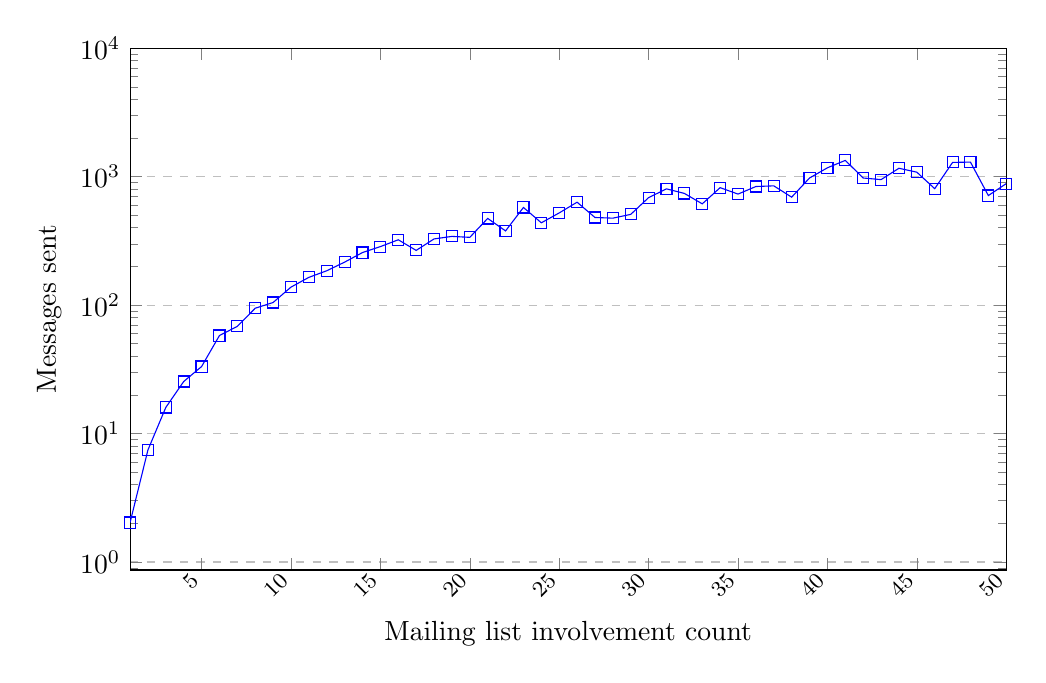
\begin{tikzpicture}
\begin{axis}[
     /pgf/number format/.cd,
     use comma,
    1000 sep={},
    width=9cm, height=6cm, 
    ylabel={Messages sent},
    xlabel={Mailing list involvement count},
    scale=1.5,
    xmin=1, xmax=50,
    ymode=log,
    ymin=0, ymax=1e4,
    x tick label style={font=\footnotesize,rotate=45, anchor=east},
    legend pos=north west,
    ymajorgrids=true,
    grid style=dashed,
]
\addplot[
    color=blue,
    mark=square,
    ]
    coordinates {
(1,2.027174534699413)(2,7.453523106659638)(3,15.975831219121378)(4,25.41044984632579)(5,33.235781137509)(6,57.94322789943228)(7,68.29384965831436)(8,94.5100154083205)(9,104.75485436893204)(10,138.0251572327044)(11,164.3822393822394)(12,185.045)(13,216.0057803468208)(14,256.4931506849315)(15,285.1896551724138)(16,322.38)(17,266.46590909090907)(18,327.3125)(19,342.5405405405405)(20,336.7258064516129)(21,472.73770491803276)(22,378.03846153846155)(23,575.22)(24,437.0888888888889)(25,521.6585365853658)(26,632.3125)(27,480.6774193548387)(28,475.0)(29,508.2903225806452)(30,686.4545454545455)(31,803.0416666666666)(32,740.0)(33,613.8)(34,820.4736842105264)(35,731.2222222222222)(36,837.5454545454545)(37,847.5263157894736)(38,692.0526315789474)(39,975.8235294117648)(40,1171.2142857142858)(41,1337.3333333333333)(42,975.5294117647059)(43,947.75)(44,1161.4545454545455)(45,1082.7777777777778)(46,805.7142857142857)(47,1290.625)(48,1296.8461538461538)(49,711.8333333333334)(50,882.4545454545455)(51,1093.625)



    };
  
   

\end{axis}
\end{tikzpicture}
\caption{Messages sent by email addresses that appear in 1-50 mailing lists.}
\end{figure}

The graph flats out at around 1000, indicating that even if someone interacts with a wide variety of mailing lists, the number of messages sent, stays around the same number. This may be due to the limited amount of time any given person can spend sending emails.

\subsection{Calculating cross talk} 

From the figure 6.10 we can see that on average an entity interacts with more than 1 mailing list, and just calculating the average in this case does not tell the entire story. In order to get a better look at cross-mailing-list interactions, some adjustment had to be made to both the code, and the definitions:\\\\
\indent
\textbf{Definition 1}\\
 
\textit{Cross talk in the context of this project is defined as “an interaction by an entity with a mailing list that is not its home"}.\\

\textbf{Definition 2}\\

\textit{An entity's home mailing list is the mailing lists in which its identifier (in this case, the email address) appears the most.}\\

With the definitions in place, calculating crosstalk is very similar to calculating the average. The only difference between the 2 is the fact that the most frequent component is ignored in one of the plots.\\


Finally, on average how many messages are sent to mailing lists that are not considered the home of an entity, and how has this developed over time?\\\\



\begin{figure}[H]
\hspace*{-0.4cm}
\centering
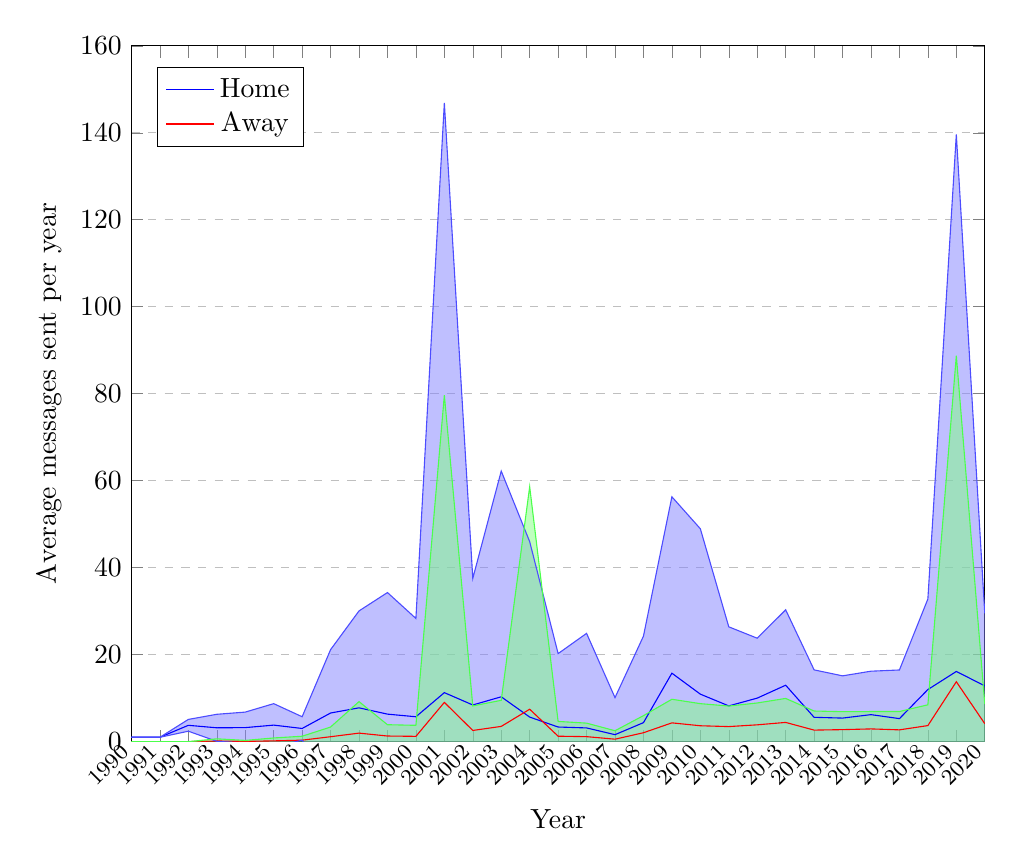
\begin{tikzpicture}
\begin{axis}[
     /pgf/number format/.cd,
     use comma,
    1000 sep={},
    width=7cm, height=6cm, 
    xlabel={Year},
    ylabel={Average messages sent  per year},
    scale=2,
    xmin=1990, xmax=2020,
    ymin=0, ymax=160,
    xtick={1980,1981,1982,1983 ,1984,1985,1986,1987,1988,1989,1990,1991,1992,1993 ,1994,1995,1996,1997,1998,1999,2000,2001,2002,2003,2004,2005,2006,2007,2008,2009,2010,2011,2012,2013,2014,2015,2016,2017,2018,2019,2020},
    x tick label style={font=\footnotesize,rotate=45, anchor=east},
    legend pos=north west,
    ymajorgrids=true,
    grid style=dashed,
]

\addplot[color=blue] coordinates {
(1990,1.0)(1991,1.0)(1992,3.75)(1993,3.1767441860465118)(1994,3.2215108834827144)(1995,3.794582392776524)(1996,3.0233766233766235)(1997,6.578186596583443)(1998,7.770768431983385)(1999,6.319893270085977)(2000,5.717015653588128)(2001,11.262751159196291)(2002,8.427462309289519)(2003,10.305207999144477)(2004,5.646533490011751)(2005,3.3577649785769474)(2006,3.1498165378063163)(2007,1.59815093300574)(2008,4.364152269987947)(2009,15.736083357122466)(2010,10.915165411071078)(2011,8.21152052238806)(2012,10.003825310806503)(2013,12.969667318982388)(2014,5.586557742294838)(2015,5.412939898018892)(2016,6.204527799356343)(2017,5.288224799286351)(2018,11.974908318857363)(2019,16.13351842503786)(2020,12.825660825660826)};\addlegendentry{Home}

\addplot[color=red] coordinates {
(1990,0.0)(1991,0.0)(1992,0.0)(1993,0.14883720930232558)(1994,0.05377720870678617)(1995,0.17474633596392333)(1996,0.33548387096774196)(1997,1.1273499090357793)(1998,1.9550683742131538)(1999,1.2872072525812137)(2000,1.2140451330414281)(2001,9.021306252489047)(2002,2.568643056108237)(2003,3.502071563088512)(2004,7.449174259681094)(2005,1.2439513022037294)(2006,1.1430809994586741)(2007,0.5591591085652243)(2008,2.042687044606362)(2009,4.314027213792121)(2010,3.646523279970671)(2011,3.458050605618619)(2012,3.861317365269461)(2013,4.416018533840807)(2014,2.6466901505100875)(2015,2.7566333519354673)(2016,2.921702481301199)(2017,2.706214990664177)(2018,3.688228299643282)(2019,13.768576742538304)(2020,4.125013612109332)};
\addlegendentry{Away}

\addplot[name path=us_top,color=blue!70] coordinates {
(1990,1.0)(1991,1.0)(1992,5.105928341272748)(1993,6.28361648619883)(1994,6.7883537893802135)(1995,8.730361095096416)(1996,5.724601647346882)(1997,21.145462195101327)(1998,30.053087109158664)(1999,34.277924047771705)(2000,28.318978030396675)(2001,146.88319352455096)(2002,37.53355750602556)(2003,62.20502422620849)(2004,45.986816318787)(2005,20.23605884444096)(2006,24.894047726099984)(2007,10.111129539206186)(2008,24.2544293769453)(2009,56.29186263021945)(2010,48.94787263164849)(2011,26.391619081263798)(2012,23.780642131463424)(2013,30.309200413817745)(2014,16.494779130474228)(2015,15.122898278554313)(2016,16.19405185273626)(2017,16.473520184977065)(2018,32.80416142798326)(2019,139.62310539455174)(2020,29.472311504750902)};


\addplot[name path=us_down,color=blue!70] coordinates {
(1990,1.0)(1991,1.0)(1992,2.3940716587272517)(1993,0.06987188589419357)(1994,-0.3453320224147842)(1995,-1.141196309543369)(1996,0.3221515994063653)(1997,-7.989089001934442)(1998,-14.511550245191895)(1999,-21.63813750759975)(2000,-16.88494672322042)(2001,-124.35769120615839)(2002,-20.67863288744652)(2003,-41.59460822791953)(2004,-34.6937493387635)(2005,-13.520528887287066)(2006,-18.59441465048735)(2007,-6.914827673194705)(2008,-15.526124836969405)(2009,-24.819695915974513)(2010,-27.117541809506328)(2011,-9.968578036487678)(2012,-3.772991509850417)(2013,-4.369865775852968)(2014,-5.32166364588455)(2015,-4.2970184825165285)(2016,-3.7849962540235724)(2017,-5.8970705864043635)(2018,-8.85434479026853)(2019,-107.35606854447602)(2020,-3.82098985342925)};


\addplot[blue!50,fill opacity=0.5] fill between[of=us_top and us_down];




\addplot[name path=div_top,color=green!70] coordinates {
(1990,0.0)(1991,0.0)(1992,0.0)(1993,0.6444425583245577)(1994,0.2813157811106731)(1995,0.8412069594535859)(1996,1.2358017706562239)(1997,3.353880239704391)(1998,9.203219187215307)(1999,3.888697199732486)(2000,3.747244603125343)(2001,79.68059769123096)(2002,8.206458157710884)(2003,9.496109236286902)(2004,58.61577301492333)(2005,4.644492135426392)(2006,4.252095224622129)(2007,2.502703694293124)(2008,5.973824939305885)(2009,9.739015781751037)(2010,8.732101165066247)(2011,8.179219588007452)(2012,8.885057628539831)(2013,9.933899481495201)(2014,7.0365925217947956)(2015,6.886481866327898)(2016,6.916233286047339)(2017,6.922928939517584)(2018,8.46461692139536)(2019,88.76168041553137)(2020,8.661465861203498)};


\addplot[name path=div_down,color=green!70] coordinates {
(1990,0.0)(1991,0.0)(1992,0.0)(1993,-0.3467681397199065)(1994,-0.1737613636971008)(1995,-0.4917142875257393)(1996,-0.5648340287207401)(1997,-1.0991804216328327)(1998,-5.293082438788999)(1999,-1.3142826945700588)(2000,-1.3191543370424865)(2001,-61.63798518625287)(2002,-3.06917204549441)(2003,-2.491966110109878)(2004,-43.71742449556114)(2005,-2.156589531018933)(2006,-1.9659332257047806)(2007,-1.3843854771626751)(2008,-1.8884508500931605)(2009,-1.110961354166795)(2010,-1.4390546051249045)(2011,-1.263118376770215)(2012,-1.16242289800091)(2013,-1.1018624138135866)(2014,-1.7432122207746206)(2015,-1.3732151624569635)(2016,-1.07282832344494)(2017,-1.5104989581892299)(2018,-1.0881603221087963)(2019,-61.22452693045477)(2020,-0.4114386369848333)};


\addplot[green!50,fill opacity=0.5] fill between[of=div_top and div_down];





\end{axis}
\end{tikzpicture}
\caption{Messages sent to an address's home mailing list, as well as any other mailing lists that are not their home. Blue and green shaded areas show the standard deviation for the "Home" and "Away" cases, respectively.}
\end{figure}





\chapter{Tracking threads}

\section{Motivation}

In order to gain better understanding of how RFCs come to be, it is vital to know
what kind of discussion usually ends with the publication of a new RFC. What kind of arguments were used? What kind of response did said arguments evoke? Were they positive, negative, or somewhere in between?\\ 




Before these questions can be answered a definition of a conversation thread needs to be specified. The simplest way of defining a conversation thread is by using the “reply-to” and “in-reply-to” fields normally found in email messages.
Like discussed in a previous chapter, these fields directly refer to another message that was sent at an earlier point in time.\\

The most recent RFC defining these fields and their inner workings is RFC~5322 \cite{RFC5322}, which describes these fields as follows\\\\




\begin{displayquote}
The "In-Reply-To:" and "References:" fields are used when creating a
   reply to a message.  They hold the message identifier of the original
   message and the message identifiers of other messages (for example,
   in the case of a reply to a message that was itself a reply).  The
   "In-Reply-To:" field may be used to identify the message (or
   messages) to which the new message is a reply, while the
   "References:" field may be used to identify a "thread" of
   conversation.\\

   When creating a reply to a message, the "In-Reply-To:" and
   "References:" fields of the resultant message are constructed as
   follows:\\

   The "In-Reply-To:" field will contain the contents of the
   "Message-ID:" field of the message to which this one is a reply (the
   "parent message").  If there is more than one parent message, then
   the "In-Reply-To:" field will contain the contents of all of the
   parents' "Message-ID:" fields.  If there is no "Message-ID:" field in
   any of the parent messages, then the new message will have no "In-
   Reply-To:" field.\\

   The "References:" field will contain the contents of the parent's
   "References:" field (if any) followed by the contents of the parent's
   "Message-ID:" field (if any).  If the parent message does not contain
   a "References:" field but does have an "In-Reply-To:" field
   containing a single message identifier, then the "References:" field
   will contain the contents of the parent's "In-Reply-To:" field
   followed by the contents of the parent's "Message-ID:" field (if
   any).  If the parent has none of the "References:", "In-Reply-To:",
   or "Message-ID:" fields, then the new message will have no
   "References:" field.\\
\end{displayquote}

Note that in the definition of the “references” field, it is stated that it can be used to track a “thread” of conversation, exactly what we are trying to do here. However, considering the note following the definition:\\




\begin{displayquote}
	Note\\
	Some implementations parse the "References:" field to
      display the "thread of the discussion".  These implementations
      assume that each new message is a reply to a single parent and
      hence that they can walk backwards through the "References:" field
      to find the parent of each message listed there.  Therefore,
      trying to form a "References:" field for a reply that has multiple
      parents is discouraged; how to do so is not defined in this
      document.

\end{displayquote}

Specifically, we cannot assume that a reply only has a single parent. Like mentioned, a thread may split at any moment for any reason, it is for this reason safer to use the “In-Reply-to” field to track threads. \\


\section{Definitions}

Before further discussing the challenges that arise when trying to track conversation threads, some definitions have to be put in place.
These definition are as follows:\\


\subsection{Node} 
A node is defined as a unique message id.\\\\


\subsection{Parent}
A parent is defined as the set of message ids contained within any given messages “In-Reply-To” field. No further restrictions are placed upon this definition, meaning that for example, a node is perfectly capable of being its own parent. \\\\


\subsection{Child}
A child is defined as a set of message ids belonging to messages that have a message id in their “In-Reply-To” field. Like with the definition of a “Parent”, a node can be its own child.\\\\

\subsection{Stub}
A stub is a node with no connecting edges.\\\\

These definitions are based on the intuitive understanding of how a conversation works, and are also based on the underlying assumption that a reply to a message cannot take place before the original message is created. \\ 

With all these definitions in place, the final product will be a one or several bidirectional graphs. From here graph traversal algorithms like Djikstras can be utilized to collect information about conversations.

\section{Extrapolating edges} 

In a perfect world there would always be a bidirectional edge from one node to another, or no edge at all. This is however not the case. This can be due to data errors, corruption, a parsing error, or the data simply missing from the very beginning. 
It is safe to assume that  if any given node A is child of node B, then node B is also parent of node A. The child of a node will always be younger than its parent and vice versa. 
For this reason, a bidirectional edge will be added between A and B as long as the criterion for at least one direction is present. \\\\







\section{Implementing the thread tracker} 

Implementing the thread tracker is best done by utilizing Solr as much as possible. The first challenge one will encounter is the fact that we do not know at what point in a thread a given message is without further investigation.
This means that the tread tracker needs the ability to “grow” the thread both forwards and backwards. This is already made possible by the definitions above.\\

The direction in which the thread tracked program decides to “grow” first is irrelevant, as the process does not create new nodes; rather, it links them. The process does not alter the existing data in any way, it simply creates new information based on what it already knows.\\

As previously mentioned, there is no real way of knowing when a “thread”, in terms of conversation related to a specific topic ends. It is absolutely possible that a thread, as defined in this project, continues for a very long time, and discusses many different topics.
One could say that the change of topic happens when the “Subject” field changes, and while this is not an unreasonable suggestion, there is no way to know for sure. There is also the problem of replies adding a “Re:” and other string to a “Subject” field without any pre-defined format. For this reason the “Subject field will not be taken into account for now.\\

It is also important to note that the result of this endeavour heavily relies on the “In-reply-to” field actually having data in it, currently the value “null” is present in 1368596 out of 2893656 documents, that being roughly 47\% of all messages. This does not necessarily mean that the data is bad, the “in-reply-to” is not a mandatory field, so the absence of data cannot be considered an error, it is perfectly possible that a lot of messages are simply never replied to.\\



\subsection{Representing the results}   

Since for the time being, only the “In-reply-to” field will be used to track down threads, a timeline representation makes some sense, as it logically speaking makes sense that a reply to a message must have been sent at a later point in time than the message being replied to.\\

This fact can potentially be used to extrapolate dates of messages that are missing them.  For example, if message A was sent on the first of november 2020, and message B, which is a reply to message A, does not have a proper date, we at least know that it is older than message A. If in addition, there is a message C, that is a reply to message B, we get a specific period of time where message B must have been sent.
This of course will not yield a perfectly accurate time, however, being able to tell the year and month when a message was sent is still a huge improvement over not being able to tell anything.\\

The problem with a timeline is the fact that a message can have several replies that may have been sent at different points in time. This fact makes a tree representation more suitable. This representation has however another weakness: for a tree to meet the requirement of being a tree, the nodes on a given level cannot be connected to each other. This is not a property that can be guaranteed in this case due to the uncertain nature of the data at hand.
With that in mind, a more accurate representation would be a graph as a graph does not have to maintain the property mentioned previously. In a graph, one is free to connect nodes in any way one pleases. 
For all these reasons the graph representation has been chosen.





\subsection{The thread tracking program} 

The following is a high level description of how the thread tracking program works.\\\\

\begin{itemize}
\item First, using Solr, obtain a list of all message ids in the database. This of course excludes all messages that do not meet this requirement, as mentioned previously.\\

\item Then for each message id, create a node object that will represent the message with a specific id. Then, for each node object, query Solr to obtain message ids for the nodes parents and children. Finally print all to a file and upload the results to a Solr core.\\
\end{itemize}


\subsection{The code, phase 1}

The first step in creating a thread tracking program is building the conversation graph. The graph building program calculates both parents, and children of all nodes. This is all finally saved to a structured file ready to be read and processed further by another program.\\

One thing to note here is that this step is strictly speaking, not necessary as all needed information regarding a node's parent and children is already stored within Solr. The process of extracting and parsing this information from Solr is a very computationally heavy task that takes several hours to complete. Essentially, what the following code is doing, can in a way be seen as caching, in order to speed up future endeavours.\\

Each node is stored as the following object.\\

\lstinputlisting[language=Python,firstline=8, lastline=15]{start_v3.py}


\textbf{\textit{id}} being the message id, \textbf{\textit{parent}} being message id’s of the parent messages, \textbf{\textit{children}} being a list of message id’s of the children, and \textbf{\textit{seen}} being simply a way to mark already seen nodes when traversing the graph.



\subsection{get\_parent()}

This is the first of 2 main methods. As the name suggest, it is this method that is responsible for calculating a given node's parents.\\ 

The query parameters are as follows:


\lstinputlisting[language=Python,firstline=52, lastline=52]{start_v3.py}






It takes two input arguments, the current node to be used as the base of the calculations, and an already set up Solr object that will be used to interface with a Solr instance of choice.

\lstinputlisting[language=Python,firstline=54, lastline=57]{start_v3.py}

Notice that this query does not make use of the facet function, and is limited to returning only 1 document at most. The underlying assumption here is that even if there are several copies of the same message in the database, they should only differ in the content of their “Mailing list” field, as all other fields are pulled directly from the mbox file. 

The “fl” parameter is also set to the “In-Reply-To-address” field in order to limit the amount of data that needs to be sent by Solr, and hence quicken execution significantly.


Next is a series of attempts at obtaining the best results from the database.
A Solr query, in this case, can fail in two different ways. 
The first is a syntax error, these are usually caused by illegal characters, and cause an exception to occur.
The other one, is the results set being empty. This is considered an error in this case, as all queries executed by this program are based on the message ids it has obtained at the start of execution from the same database, meaning that every message id should at the very least have one message associated with it.
Both of these errors, however, have the same solution. The solution is the message id with quotation marks, as this makes Solr parse the query string as one “unit”. This is still not enough, as some message id-s contain a colon. This is a reserved character that cannot occur in queries, unless escaped with a  backslash.
Any backslashes that are in the original message id also need to be escaped with the same backslash.


If any errors are encountered on the first try, the message-id is slightly modified as described above, and a new attempt is made. If this attempt also fails, the message id is logged as an error, printed to the terminal, and printed to a log file at the end of execution for further investigation.



\lstinputlisting[language=Python,firstline=60, lastline=66,   breaklines=true]{start_v3.py}

Recall that the fl parameter refers to the “In-Reply-To-address” field in the database, now recall from chapter 5, that said field is a multivalued field, which Solr returns as a Python list. If a satisfactory response is obtained from Solr, this list is iterated over to check if an element in the list is a message id that matched one of the messages obtained at the start of execution. 
This may sometimes fail as message ids are usually surrounded by a less-than and greater-than sign. This is in some cases removed during parsing. In order to ensure the best possible result, a second attempt at matching the element is made; this time, with the surrounding characters added back in.
If the second attempt fails, the element is ignored.\\



\lstinputlisting[language=Python,firstline=104, lastline=117, breaklines=true]{start_v3.py}



\subsection{get\_child()}


This is the second method, and as the name suggests its purpose is to get the children of a given node. Its input arguments are the exact same as with the previous method, the node whose children we want to calculate, and a Solr object that will be used to communicate with Solr. In contrast to the get\_parent() method, this one utilizes Solr’s facet function. The following is the parameter list used for queries in this method


\lstinputlisting[language=Python,firstline=125, lastline=132,   breaklines=true]{start_v3.py}



The get\_child() method follows the same philosophy in terms of obtaining the best possible result from the database, meaning it makes several attempts if the previous one was not satisfactory.

The first attempt is made with the unmodified message id found in the node object passed to the function. If this query returns 0 results, one of 2 actions is taken based on the format of the id string. Like mentioned in the previous method, message ids are usually surrounded by a greater-than and less-than sign like so “<messageid>”.
These 2 surrounding characters are in some cases removed during the parsing process. This method queries the “In-Reply-To-address” field, meaning that using values from the “Message-ID” field directly has a chance of not actually matching anything. If this happens and the message id has the previously mentioned format, a new attempt is made with the first and last character of the message id removed, as well as the illegal characters.


\lstinputlisting[language=Python,firstline=138, lastline=143,   breaklines=true]{start_v3.py}



If more than 2 attempts fail, the message is printed to a file as well as the terminal for further investigation at a later point.

Finally, since the facet function is used, the list returned by Solr needs to have the facet counts removed. While this is happening, the program, like in the “get\_parent()” method, matches the message ids against the very first list  of message ids obtained at the start. If a match is found, the message id is added to the parent list of the input node.




\lstinputlisting[language=Python,firstline=175, lastline=188,   breaklines=true]{start_v3.py}


With these two methods in place, it is now possible to build a graph of conversations held across the IETF.




\subsection{Removing stubs}
There is room to improve this approach. First of all, since the goal is to track a conversation, nodes that have no incoming or outgoing edges can be omitted, as they can only be accessed from themselves, and are not part of any other tree/graph. Doing this will decrease the amount of data that needs to be stored.\\

This is done by the thread tracking program right after phase 1, when writing the results to a file.  


\subsection{The save format}

Due to the uncertain nature of data in this project, a well structured way of saving the graphs and nodes to a file had to be created. This format ensures that all nodes and graphs are read and written correctly. 
The format in both nodes and graphs is based on delimiters that were chosen by trial and error, and do not appear in the “Message-ID” field at any point. If these characters are to appear in any future iterations of the database, the save format will have to be adjusted to account for this.\\\\
The delimiter characters, and what they mean is as follows.\\

\textbf{Nodes}\\

\begin{description}


\item[\( \Delta \)] = start of a node, this character is always followed by the message-id of said node.\\

\item[\( \lambda \)] = marks the end of a nodes message-id.\\

\item[\( \Gamma \)] p = marks the start of a node's parents, all following nodes are to be assigned accordingly \\

\item[\( \Gamma \)]  c = marks the start of a node's children, all following nodes are to be assigned accordingly \\

\item[\( \alpha \)] = marks the start of a message id that is either a child or a parent of the current node \\

\item[\( \Omega \)] = marks the end of a message id that is either a child or a parent of the current node\\

\item[\( \S \)] = marks the end of a node. When this character is encountered, the node should have been read in its entirety. This character is always followed by two empty lines.\\

\end{description}

\noindent
Example:

\begin{quotation}

\noindent
\( \Delta \)\\
<200207032102.g63L2B203351@astro.cs.utk.edu>\\
\( \lambda \)\\
\( \Gamma \)p\\
\( \alpha \)\\
<5.1.0.14.2.20020703172727.03e210d0@joy.songbird.com>\\
\( \Omega \)\\
\( \Gamma \)c\\
\( \alpha \)\\
<A8SJGB6GEA6YSYUNJ1ZLFDA1U3YTRNL.3d25477c@www>\\
\( \Omega \)\\
\( \alpha \)\\
<20020708100834.A13615@bailey.dscga.com>\\
\( \Omega \)\\
\( \alpha \)\\
<5.1.0.14.2.20020704000946.039f2780@joy.songbird.com>\\
\( \Omega \)\\
\( \S \) \\

\end{quotation}

\textbf{Graphs:}\\

As previously mentioned, trees are ascribed their own unique id, this id is always the first thing that is read, and also function as a delimiter.

\begin{description}


\item[---(int)] = The start of a tree, the “(int)” can be replaced with any integer, this line is always followed by an empty line, then another integer signifying the current level.\\

\item[\( \alpha \)] = Same as nodes \\


\item[\( \Omega \)] = Same as nodes\\


\item[\( \Delta \)] = Signifies the end of a level \\


\item[\( \S \)] = Signifies the end of a tree, this character is always followed by exactly 4 empty lines 

\end{description}

\subsection{Solr cores}
Two new Solr cores were made as well in order to accommodate the results of this calculation. The cores are aptly named “graphs” and “nodes”. Documents contained within the “graphs” core only have four fields, two of which are automatically added by Solr, and bear no difference on the other fields:\\

Graphs:

\begin{itemize}
\item \emph{graph-id}\\
This field contains the id number of a given graph

\item \emph{nodes}\\
This is a multivalued field, it contains message id’s of all nodes that belong to a graph.\\


\end{itemize}

The two fields added by Solr are “id” and “version”.\\

The “nodes” core contains documents that have 5 or 6 fields. Since Solr is perfectly capable of searching for documents that are missing a specific field, it was chosen to omit default values for fields in this core. For example, if a node does not have any parent, instead of its “parent” field containing a default value, which was up to now “Null”, the field will simply be missing. 
In order to query Solr for documents that do not have a certain field, a “-” sign  must be placed before the name of the field when writing the query.
For example, the following query will return all documents without the “parent” field.\\ 

\begin{center}
-parent:*
\end{center}

With that cleared up, the documents in the “nodes” core have the following fields.


\begin{itemize}

\item node-id\\ 
This is the id that uniquely identifies a message. For each unique value in this field, there is at least one message in the main database core. The same message can appear in several places. Announcement messages for example, sent to several mailing lists, will have several “copies” in the database, with the difference being the contents of their  “Mailing-lists” content. There could be other differences as well since the messages were parsed from different files, the parsing process itself may have had varying degrees of success in extracting the data. This is just one of many instances where the database could be improved upon. Tracking down copies of the same messages in different places, then using the extracted data to form one complete document. The “Mailing-list” field could for example be changed to a multivalued field that would contain names of all mailing lists said message had been found in. Doing this may also improve the results of tracking threads.  


\item graph-id \\
This field simply indicates which graph a node belongs to. For each node, there is exactly one graph it belongs to.

\item Parent and child\\
These two fields are both functionally equal. They are both multi valued fields in the database, and contain message ids of other nodes. Notice the difference between a node-id and a message-id.  A message-id, as found in the main database core, is a value directly extracted by the parser, belonging to a message. A node id is a message-id that has at least one connection/edge to another node. For each node-id, there is always a corresponding document in the main core, this is however not the case the other way around.


\end{itemize}

The two automatically added fields are present here as well.\\

Finally, the two cores have the following tokenizers for their non-standards fields:

\begin{center}

Graphs:
\begin{center}
 \begin{tabular}{||c c||} 
 \hline
 \textit{Field} & \textit{Tokenizer} \\ [1ex] 
 \hline\hline

graph-id & No tokenizer\\

\hline

nodes & solr.KeywordTokenizerFactory\\

\hline

\end{tabular}
\end{center}


Nodes:
\begin{center}
 \begin{tabular}{||c c||} 
 \hline
 \textit{Field} & \textit{Tokenizer} \\ [1ex] 
 \hline\hline


node-id & solr.KeywordTokenizerFactory\\

\hline

graph-id & No tokenizer\\

\hline

parent & solr.KeywordTokenizerFactory\\

\hline

child & solr.KeywordTokenizerFactory\\

\hline

\end{tabular}
\end{center}

\begin{flushleft}
With the layout of the nodes in place, here are some statistics regarding the data contained within. 
\end{flushleft}


\begin{figure}[H]
\hspace*{-0.5cm}
\centering
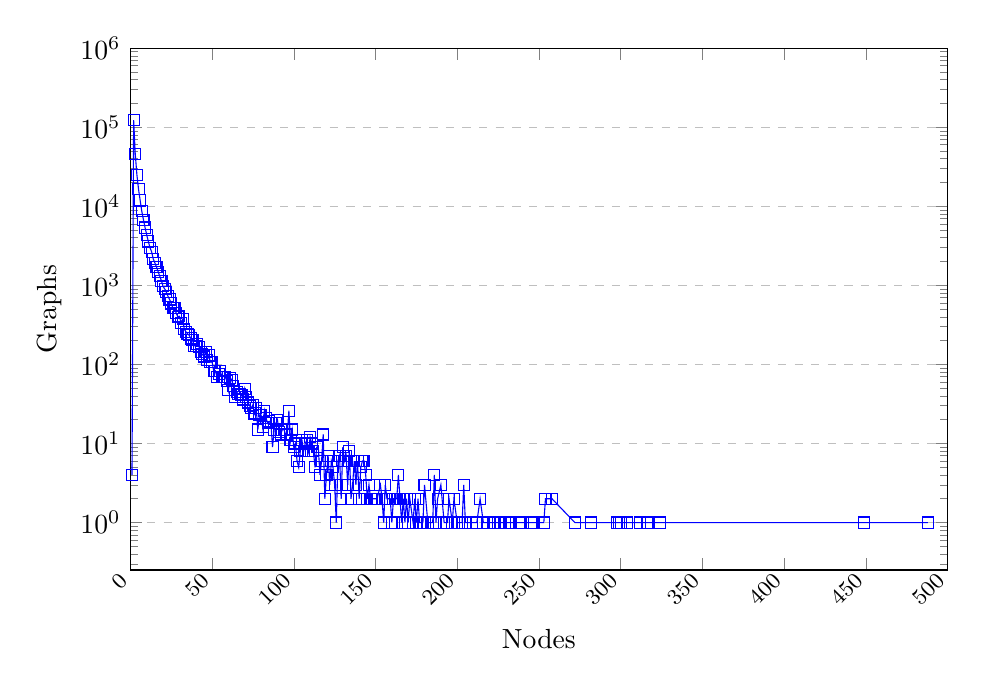
\begin{tikzpicture}
\begin{axis}[
     /pgf/number format/.cd,
     use comma,
    1000 sep={},
    width=8.5cm, height=6cm, 
    xlabel={Nodes},
    ylabel={Graphs},
    scale=1.5,
    xmin=0, xmax=500,
    ymode=log,
    ymin=0, ymax=1e6,
    x tick label style={font=\footnotesize,rotate=45, anchor=east},
    legend pos=north west,
    ymajorgrids=true,
    grid style=dashed,
]
\addplot[
    color=blue,
    mark=square,
    ]
    coordinates {
(1,4)(2,123015)(3,45537)(4,25069)(5,16409)(6,11851)(7,8645)(8,6758)(9,5387)(10,4355)(11,3593)(12,2994)(13,2666)(14,2161)(15,1926)(16,1707)(17,1483)(18,1304)(19,1148)(20,971)(21,903)(22,823)(23,728)(24,663)(25,591)(26,513)(27,514)(28,448)(29,402)(30,406)(31,337)(32,373)(33,280)(34,258)(35,245)(36,234)(37,213)(38,203)(39,173)(40,171)(41,183)(42,167)(43,142)(44,135)(45,126)(46,144)(47,113)(48,130)(49,107)(50,108)(51,82)(52,83)(53,70)(54,76)(55,83)(56,70)(57,70)(58,70)(59,62)(60,47)(61,68)(62,64)(63,53)(64,39)(65,45)(66,42)(67,42)(68,41)(69,36)(70,49)(71,39)(72,33)(73,30)(74,28)(75,31)(76,24)(77,28)(78,15)(79,23)(80,23)(81,16)(82,26)(83,21)(84,18)(85,19)(86,18)(87,9)(88,15)(89,18)(90,20)(91,14)(92,13)(93,15)(94,15)(95,13)(96,13)(97,26)(98,11)(99,15)(100,9)(101,10)(102,6)(103,5)(104,8)(105,11)(106,8)(107,10)(108,11)(109,8)(110,12)(111,10)(112,8)(113,5)(114,9)(115,9)(116,4)(117,6)(118,13)(119,2)(120,4)(121,7)(122,3)(123,6)(124,5)(125,3)(126,1)(127,6)(128,7)(129,2)(130,9)(131,6)(132,7)(133,3)(134,8)(135,2)(136,3)(137,6)(138,3)(139,6)(140,2)(141,5)(142,6)(143,6)(144,4)(145,2)(146,3)(147,2)(148,2)(149,2)(150,2)(151,2)(153,3)(154,2)(155,1)(156,3)(157,2)(159,2)(160,1)(161,2)(162,2)(163,2)(164,4)(165,2)(166,1)(167,2)(168,1)(169,2)(170,1)(171,2)(173,1)(174,2)(175,1)(176,2)(177,1)(178,1)(179,1)(180,3)(182,1)(185,1)(186,4)(187,1)(188,2)(190,3)(192,1)(193,1)(194,1)(195,2)(197,1)(198,2)(200,1)(201,1)(203,1)(204,3)(205,1)(212,1)(214,2)(216,1)(218,1)(222,1)(223,1)(226,1)(227,1)(229,1)(232,1)(233,1)(238,1)(245,1)(246,1)(247,1)(253,1)(254,2)(258,2)(272,1)(282,1)(298,1)(299,1)(300,1)(304,1)(312,1)(316,1)(317,1)(324,1)(449,1)(488,1)
    };
  
    
\end{axis}
\end{tikzpicture}
\caption{The number of graphs of a certain length contained in the database.}
\end{figure}





\begin{figure}[H]
\hspace*{-0.5cm}
\centering
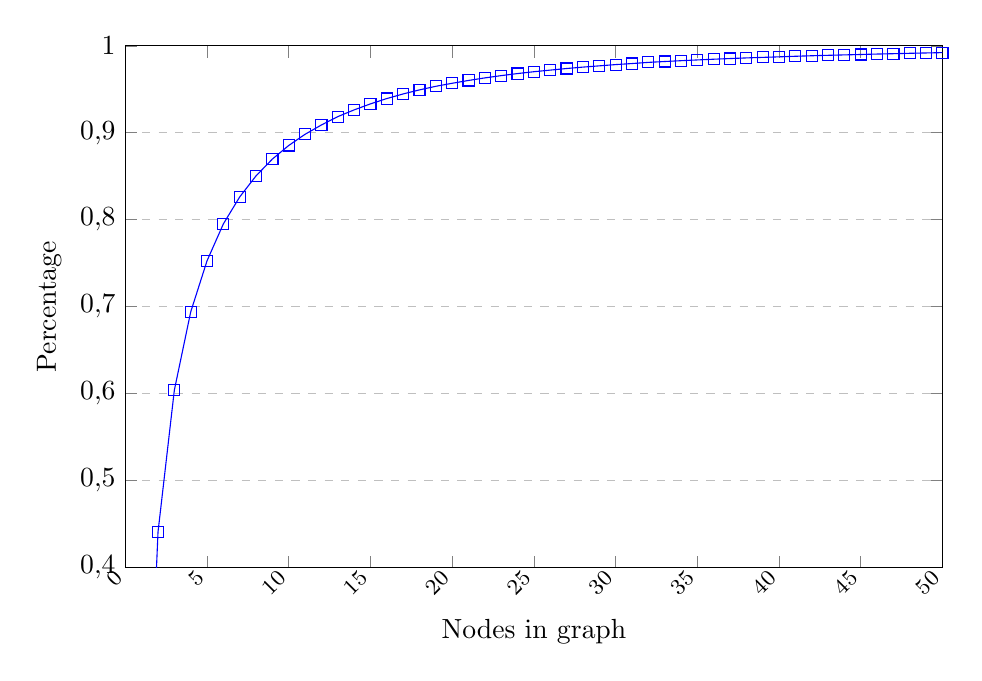
\begin{tikzpicture}
\begin{axis}[
     /pgf/number format/.cd,
     use comma,
    1000 sep={},
    width=8.5cm, height=6cm, 
    xlabel={Nodes in graph},
    ylabel={Percentage},
    scale=1.5,
    xmin=0, xmax=50,
    ymin=0.4, ymax=1,
    x tick label style={font=\footnotesize,rotate=45, anchor=east},
    legend pos=north west,
    ymajorgrids=true,
    grid style=dashed,
]
\addplot[
    color=blue,
    mark=square,
    ]
    coordinates {
(1,1.4336763403977734e-05)(2,0.4409235742984842)(3,0.6041368730802178)(4,0.6939889535237972)(5,0.7528019411977649)(6,0.7952781869729)(7,0.8262635168797469)(8,0.8504854786507672)(9,0.8697935147650742)(10,0.885402665921155)(11,0.898280663648778)(12,0.9090117310566553)(13,0.9185671838654065)(14,0.9263126202944054)(15,0.9332157718734208)(16,0.9393339856560682)(17,0.9446493406880929)(18,0.9493231255577897)(19,0.9534377766547313)(20,0.9569180259710469)(21,0.9601545503094949)(22,0.9631043393798633)(23,0.9657136303193873)(24,0.9680899488535966)(25,0.9702082056465343)(26,0.9720468955530944)(27,0.9738891696505055)(28,0.975494887151751)(29,0.9769357318738509)(30,0.9783909133593546)(31,0.9795987856761397)(32,0.9809356888635606)(33,0.981939262301839)(34,0.9828639835413956)(35,0.9837421102998892)(36,0.984580810959022)(37,0.9853442436102837)(38,0.9860718343530356)(39,0.9866918993702577)(40,0.9873047960057777)(41,0.9879607029315097)(42,0.9885592628036257)(43,0.989068217904467)(44,0.9895520836693512)(45,0.9900036917165765)(46,0.9905198151991197)(47,0.9909248287652821)(48,0.9913907735759113)(49,0.9917742819969678)(50,0.9921613746088752)(51,0.9924552782586568)(52,0.9927527660992893)(53,0.9930036594588588)(54,0.9932760579635345)(55,0.993573545804167)(56,0.9938244391637366)(57,0.9940753325233062)(58,0.9943262258828758)(59,0.9945484457156375)(60,0.9947169026856342)(61,0.9949606276635018)(62,0.9951900158779655)(63,0.9953799779930682)(64,0.995519761436257)(65,0.9956810500245518)(66,0.9958315860402934)(67,0.9959821220560352)(68,0.996129073880926)(69,0.9962581047515618)(70,0.9964337301032605)(71,0.9965735135464493)(72,0.9966917918445322)(73,0.996799317570062)(74,0.9968996749138899)(75,0.9970107848302706)(76,0.9970968054106945)(77,0.9971971627545223)(78,0.9972509256172872)(79,0.9973333620068602)(80,0.997415798396433)(81,0.997473145450049)(82,0.9975663344121748)(83,0.9976416024200456)(84,0.9977061178553636)(85,0.9977742174815325)(86,0.9978387329168503)(87,0.9978709906345093)(88,0.9979247534972743)(89,0.9979892689325921)(90,0.998060952749612)(91,0.998111131421526)(92,0.9981577259025889)(93,0.9982114887653538)(94,0.9982652516281187)(95,0.9983118461091817)(96,0.9983584405902446)(97,0.9984516295523704)(98,0.9984910556517314)(99,0.9985448185144963)(100,0.9985770762321552)(101,0.9986129181406651)(102,0.9986344232857711)(103,0.9986523442400261)(104,0.998681017766834)(105,0.998720443866195)(106,0.998749117393003)(107,0.9987849593015129)(108,0.9988243854008738)(109,0.9988530589276818)(110,0.9988960692178938)(111,0.9989319111264037)(112,0.9989605846532116)(113,0.9989785056074666)(114,0.9990107633251255)(115,0.9990430210427845)(116,0.9990573578061884)(117,0.9990788629512944)(118,0.9991254574323574)(119,0.9991326258140594)(120,0.9991469625774633)(121,0.9991720519134203)(122,0.9991828044859733)(123,0.9992043096310792)(124,0.9992222305853342)(125,0.9992329831578872)(126,0.9992365673487382)(127,0.9992580724938441)(128,0.9992831618298011)(129,0.9992903302115032)(130,0.9993225879291621)(131,0.999344093074268)(132,0.999369182410225)(133,0.999379934982778)(134,0.9994086085095859)(135,0.9994157768912879)(136,0.9994265294638409)(137,0.9994480346089468)(138,0.9994587871814998)(139,0.9994802923266058)(140,0.9994874607083079)(141,0.9995053816625628)(142,0.9995268868076688)(143,0.9995483919527747)(144,0.9995627287161787)(145,0.9995698970978807)(146,0.9995806496704337)(147,0.9995878180521356)(148,0.9995949864338376)(149,0.9996021548155396)(150,0.9996093231972416)(151,0.9996164915789436)(153,0.9996272441514966)(154,0.9996344125331985)(155,0.9996379967240495)(156,0.9996487492966025)(157,0.9996559176783045)(159,0.9996630860600065)(160,0.9996666702508575)(161,0.9996738386325595)(162,0.9996810070142615)(163,0.9996881753959634)(164,0.9997025121593675)(165,0.9997096805410695)(166,0.9997132647319205)(167,0.9997204331136225)(168,0.9997240173044735)(169,0.9997311856861755)(170,0.9997347698770264)(171,0.9997419382587284)(173,0.9997455224495794)(174,0.9997526908312814)(175,0.9997562750221324)(176,0.9997634434038344)(177,0.9997670275946854)(178,0.9997706117855364)(179,0.9997741959763874)(180,0.9997849485489403)(182,0.9997885327397913)(185,0.9997921169306423)(186,0.9998064536940463)(187,0.9998100378848973)(188,0.9998172062665993)(190,0.9998279588391523)(192,0.9998315430300032)(193,0.9998351272208542)(194,0.9998387114117052)(195,0.9998458797934072)(197,0.9998494639842582)(198,0.9998566323659602)(200,0.9998602165568112)(201,0.9998638007476622)(203,0.9998673849385132)(204,0.9998781375110661)(205,0.9998817217019171)(212,0.9998853058927681)(214,0.9998924742744701)(216,0.9998960584653211)(218,0.9998996426561721)(222,0.9999032268470232)(223,0.9999068110378742)(226,0.9999103952287252)(227,0.9999139794195762)(229,0.9999175636104272)(232,0.9999211478012782)(233,0.9999247319921292)(238,0.9999283161829801)(245,0.9999319003738311)(246,0.9999354845646821)(247,0.9999390687555331)(253,0.9999426529463841)(254,0.9999498213280861)(258,0.9999569897097881)(272,0.9999605739006391)(282,0.9999641580914901)(298,0.9999677422823411)(299,0.9999713264731921)(300,0.9999749106640431)(304,0.999978494854894)(312,0.999982079045745)(316,0.999985663236596)(317,0.999989247427447)(324,0.999992831618298)(449,0.999996415809149)(488,1.0)
    };
  
    
\end{axis}
\end{tikzpicture}
\caption{
Cumulative Distribution Function of graphs contained in the database, for graphs containing up to 50 nodes.
}
\end{figure}





\end{center}


As we can see from the figures above, the vast majority of graphs in the database are quite small, usually being only 2 to 4 nodes large. This means that extracting conversations from these graphs is going to be limited, and it should be expected that the conversation tracking process will reflect this fact.

\section{Returning a subgraph }
Before a conversation thread can be calculated from the newly obtained data, a better idea of exactly how the tracking process will function is needed. 
The assumption here is that a user who is interested in a particular topic, would want a conversation on said topic. This by itself is not trivial, as the current implementation of the database only returns documents that represent a single message. Before we are able to return a conversation thread, a definition of a start and end of a thread needs to be defined.
This definition will depend on what exactly one is looking for, and should anyone wish to continue this work, alternative definitions of these will be a good place to start experimenting. For now, the definition will be based on their intuitive understanding, while keeping in mind the currently available data as well as the database implementation.\\



A natural way to search for a message related to a specific topic would probably be to use the “Subject” field. Its use is defined in RFC 822 \cite{RFC0822}

\url{https://tools.ietf.org/html/rfc822#section-4.7.1}


\begin{displayquote}

4.7.1.  SUBJECT
     
             This is intended to provide a summary,  or  indicate  the
        nature, of the message.



\end{displayquote}

So, given the assumption that most people use this field in the way it's meant to be used, it should be a good indicator of when the topic of a conversation changes. \\

Another field that is most likely used to discuss a certain topic, is the “Content” field. This is this field that contains the actual message the email is trying to convey. In the database, it is this field that holds the message body.
The body of a message, does not have a strict definition, and is generally defined as “unstructured text”.\\

Another potential source of information on a topic relevant to a message are the attachments of a given message. Like discussed in chapter 5, these are not included in the current implementation of the database. Should anyone wish to continue this project however, the attachments, their restoration, and analysis is certainly one area to potentially research further.\\

This finally means that there are two fields in the database that can be used to, to some degree, obtain information regarding the nature of the message. The goal of this project is to obtain better understanding of how internet standards come to be. A potential user will likely search for a specific topic. But how does one link a search, with the conversation graphs? This is certainly up for debate, but here is how it was done for this project.\\

\subsection{Linking queries to conversation graphs}


In order to link a regular Solr query to the conversation graph, a query is needed. For the sake of example, the “last call” will be used as the query term, as these imply urgency, possibly referring to the publication or submission of an RFC.\\

First, a facet query on the field “Message-ID”  with the term “last call” is made, on either the “Subject” field, the “Content” field or both, is executed.  As Solr uses cosine similarity to calculate results, it may be beneficial to require the query term to be present in both fields, as it may increase accuracy.
This query will then return a list of message ids relevant to the query term.\\

This list will then be matched with the conversation graphs, where a matching program will attempt to fetch all conversation sequences relevant to the search results. \\

\subsection{Feature requirements}

In order for this to be done quickly and efficiently, there are certain requirements that need to be satisfied.

\begin{itemize}
\item a quick way to look up which graph any given node belongs to. 
\item a quick way to look up nodes in any given graph. 
\end{itemize}


The first requirement is best solved by, yet again, using Solr. A new core has been created for this purpose. This, in contrast to many other already established cores, is a very simple one. The schema consists of only three fields: the tree id, a multivalued field containing ids of all nodes belonging to a tree, and the default Solr documents id field. This makes it possible to query the multivalued field for ids obtained from the first query, and quickly determine which graphs are relevant to said query.


The second requirement can be reasonably solved in two different ways. Recall that the conversation graph program prints its results to a structured file, said file can be read and searched as needed. The other alternative is to yet again create a new Solr core. This core would need to have a schema that can replicate the node format previously defined in the conversation graph program. This is a simple task, as the nodes object variables are easily replicable by multivalued fields in Solr. Since Solr has been a mainstay in this project, the second option was chosen.


\subsection{The conversation tracking program}


The following is a high level description of how the program in charge of calculating the results will function.


\begin{enumerate}

\item Execute a facet query on the “Message-ID” field, with the desired query term on the “Subject” and/or “Content” fields as previously discussed.
\item Convert the results of this query into a set of message ids.
\item Match the contents of said set with the query holding the conversation graphs, and determine which messages belong to which graph.
\item For each returned graph, try to find a path through all of the messages belonging to said graph, with a predetermined look ahead of at least 1. 
\item Return all paths of length of more than 1.


\end{enumerate}

The results returned by this program can finally be used to attempt to match their nodes with the publications of new RFC.\\

\subsection{Ordering a graph}

With the general idea of how the process of calculating a thread will work, it is now possible to properly define the start and end of a thread. There is, however, not one definition that is perfect. A natural way of picking a starting point for a conversation could simply be the oldest message in said conversation, this is not always correct however, as there are many messages in the database that either do not have a date, or have a date that is clearly wrong, be that messages from the future, or messages from a time long the invention of.

Another definition could be the same as that of a root, as previously defined. This has another problem however. That definition yet again hinges on the assumption of sequential flow of time. The assumption made when making said definition a node's child is always younger than its parent simply does not hold if we go by dates found in the database.

Another definition of the start of a thread, that does not depend on date, could instead depend on the parent/child relation. This is still not a perfect way of defining a start, as it is possible to send a reply to a message before the message being replied to is sent, if said messages message-id is known beforehand. This is simply something that will have to be kept in mind. This is not something that happens by accident, and it is highly unlikely that a legitimate participant of the IETF would orchestrate such a situation.\\


With all those things in mind, two options were considered as to how to sort the subgraphs returned by the thread tracing program. 

The first option is simply using the dates attached to each node. Given a subgraph, the nodes will be sorted from oldest to youngest and displayed in this order.
The second option is an enhanced version of option 1. As not all nodes have legitimate dates, if such a node is found, the program will attempt to retrieve a better date, or, at the very least, an interval of time for said node. This new period of time will be calculated based on its immediate neighbours, that being its parents and children. The program will attempt to find the smallest interval possible that does not violate the rules of sequential flow of time. This means that, children of a node that are older than parent nodes will be ignored, and vice versa.

\subsection{The results}

The following graphs depict some statistic regarding the resulting conversation threads.\\\\
\noindent
Amount of conversations found = 23254\\
Average length = 4.567945299733379\\
Standard deviation = 6.931045907316653\\


\begin{figure}[H]
\hspace*{-0.5cm}
\centering
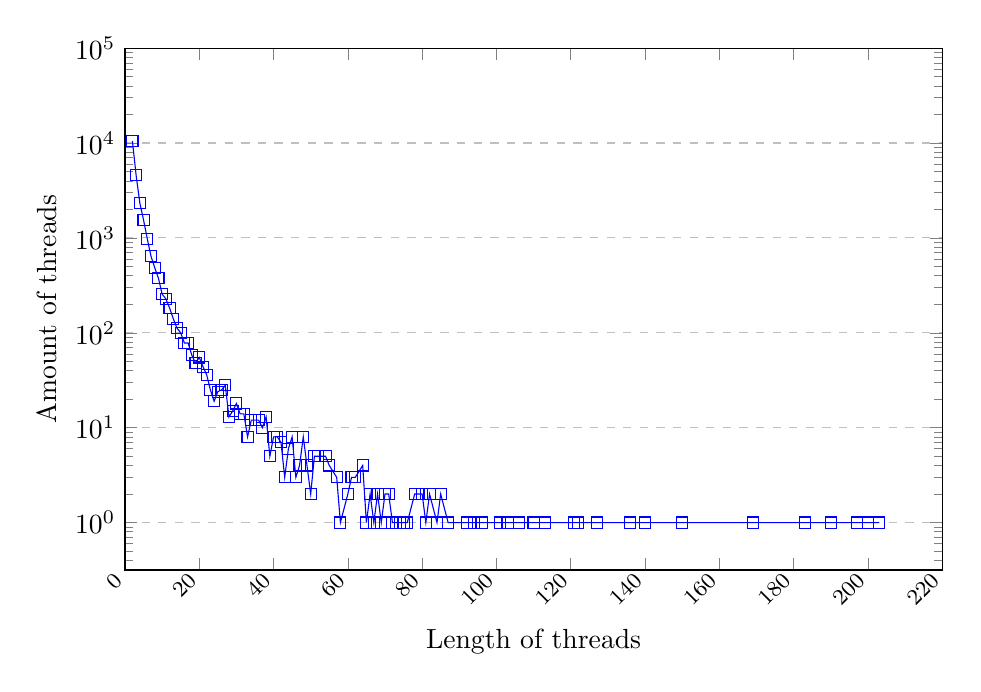
\begin{tikzpicture}
\begin{axis}[
     /pgf/number format/.cd,
     use comma,
    1000 sep={},
    width=8.5cm, height=6cm, 
    xlabel={Length of threads},
    ylabel={Amount of threads},
    scale=1.5,
    xmin=0, xmax=220,
    ymode=log,
    ymin=0, ymax=1e5,
    x tick label style={font=\footnotesize,rotate=45, anchor=east},
    legend pos=north west,
    ymajorgrids=true,
    grid style=dashed,
]
\addplot[
    color=blue,
    mark=square,
    ]
    coordinates {
(2,10493)(3,4572)(4,2329)(5,1547)(6,980)(7,643)(8,486)(9,377)(10,256)(11,228)(12,183)(13,141)(14,112)(15,100)(16,78)(17,78)(18,58)(19,48)(20,55)(21,44)(22,36)(23,25)(24,19)(25,24)(26,25)(27,28)(28,13)(29,15)(30,18)(31,14)(32,14)(33,8)(34,12)(35,12)(36,12)(37,10)(38,13)(39,5)(40,8)(41,8)(42,7)(43,3)(44,6)(45,8)(46,3)(47,4)(48,8)(49,4)(50,2)(51,5)(52,5)(54,5)(55,4)(57,3)(58,1)(60,2)(61,3)(62,3)(64,4)(65,1)(66,2)(67,1)(68,2)(69,1)(70,2)(71,2)(72,1)(73,1)(74,1)(75,1)(76,1)(78,2)(80,2)(81,1)(82,2)(84,1)(85,2)(87,1)(92,1)(94,1)(96,1)(101,1)(103,1)(106,1)(110,1)(113,1)(121,1)(122,1)(127,1)(136,1)(140,1)(150,1)(169,1)(183,1)(190,1)(197,1)(200,1)(203,1)
    };
  
    
\end{axis}
\end{tikzpicture}
\caption{The length distribution of found conversation threads}
\end{figure}












\begin{figure}[H]
\hspace*{-0.5cm}
\centering
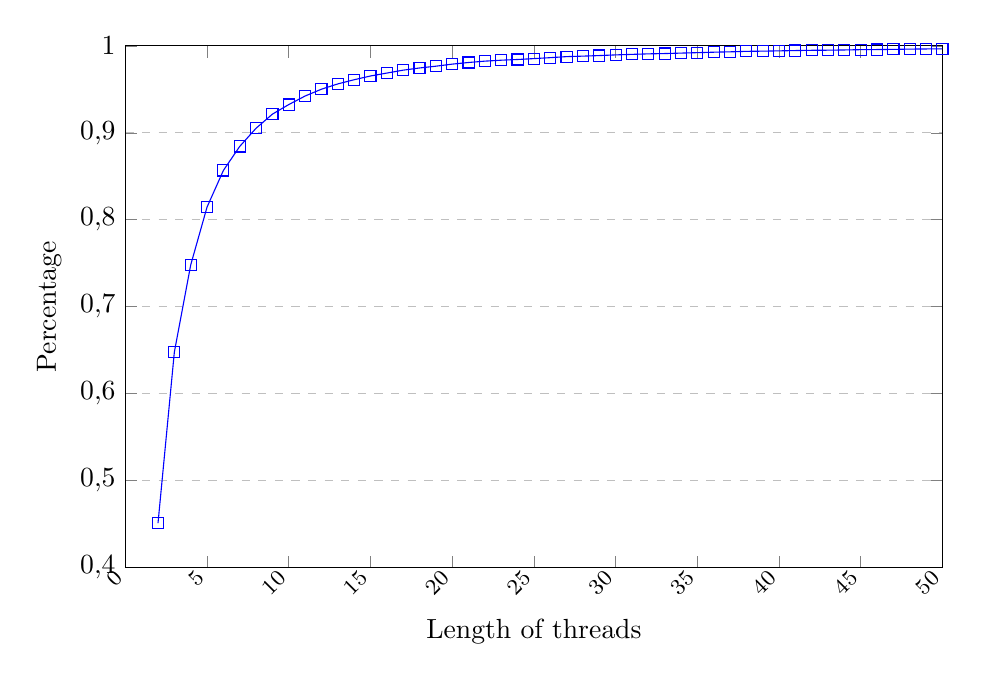
\begin{tikzpicture}
\begin{axis}[
     /pgf/number format/.cd,
     use comma,
    1000 sep={},
    width=8.5cm, height=6cm, 
    xlabel={Length of threads},
    ylabel={Percentage},
    scale=1.5,
    xmin=0, xmax=50,
    ymin=0.4, ymax=1,
    x tick label style={font=\footnotesize,rotate=45, anchor=east},
    legend pos=north west,
    ymajorgrids=true,
    grid style=dashed,
]
\addplot[
    color=blue,
    mark=square,
    ]
    coordinates {
(2,0.4512341962673089)(3,0.6478455319514922)(4,0.7480003440268341)(5,0.8145265330695795)(6,0.8566698202459792)(7,0.8843209770362088)(8,0.9052206072073622)(9,0.9214328717639976)(10,0.9324417304549755)(11,0.9422464952266276)(12,0.9501161090565065)(13,0.9561795820073966)(14,0.9609959576846994)(15,0.9652962931108626)(16,0.96865055474327)(17,0.9720048163756773)(18,0.974499010922852)(19,0.9765631719274104)(20,0.9789283564118001)(21,0.980820503999312)(22,0.9823686247527307)(23,0.9834437086092715)(24,0.9842607723402426)(25,0.9852928528425218)(26,0.9863679366990625)(27,0.9875720306183883)(28,0.9881310742237894)(29,0.9887761245377139)(30,0.9895501849144234)(31,0.9901522318740862)(32,0.990754278833749)(33,0.9910983056678421)(34,0.9916143459189817)(35,0.9921303861701213)(36,0.9926464264212609)(37,0.9930764599638772)(38,0.9936355035692784)(39,0.9938505203405865)(40,0.9941945471746796)(41,0.9945385740087727)(42,0.9948395974886041)(43,0.994968607551389)(44,0.9952266276769588)(45,0.9955706545110519)(46,0.9956996645738367)(47,0.9958716779908833)(48,0.9962157048249763)(49,0.9963877182420229)(50,0.9964737249505461)(51,0.9966887417218543)(52,0.9969037584931625)(54,0.9971187752644707)(55,0.9972907886815171)(57,0.9974197987443021)(58,0.9974628020985636)(60,0.997548808807087)(61,0.9976778188698718)(62,0.9978068289326567)(64,0.9979788423497032)(65,0.9980218457039649)(66,0.9981078524124882)(67,0.9981508557667498)(68,0.9982368624752731)(69,0.9982798658295347)(70,0.998365872538058)(71,0.9984518792465812)(72,0.9984948826008428)(73,0.9985378859551045)(74,0.9985808893093662)(75,0.9986238926636277)(76,0.9986668960178894)(78,0.9987529027264127)(80,0.9988389094349359)(81,0.9988819127891976)(82,0.9989679194977208)(84,0.9990109228519825)(85,0.9990969295605057)(87,0.9991399329147673)(92,0.999182936269029)(94,0.9992259396232906)(96,0.9992689429775522)(101,0.9993119463318139)(103,0.9993549496860755)(106,0.9993979530403372)(110,0.9994409563945987)(113,0.9994839597488604)(121,0.9995269631031221)(122,0.9995699664573837)(127,0.9996129698116453)(136,0.9996559731659069)(140,0.9996989765201686)(150,0.9997419798744303)(169,0.9997849832286918)(183,0.9998279865829535)(190,0.9998709899372151)(197,0.9999139932914768)(200,0.9999569966457383)(203,1.0)
    };
  
    
\end{axis}
\end{tikzpicture}
\caption{Cumulative distribution function of the length of conversation threads, for threads containing up to 50 nodes.
}
\end{figure}





As an example, let us take a look at a short 2 node thread from the “last call” result set.
The current implementation of the thread tracker only outputs the message ids and dates, meaning it is impossible to read the thread directly from the terminal. For this reason the content field, along with a few other select fields have been chosen to be displayed below.\\\\





2012-12-13 19:45:31 

\begin{displayquote}
\noindent
From-name =>['Ted Lemon']\\
From-address =>['Ted.Lemon@nominum.com']\\\\



\noindent
> Personally, I prefer minimizing the new message headers, and\\
> using options where possible.=20\\\\
\noindent
It seems to me that we have three people saying they\'d like to use an exist=
ing header format, one saying we should define a new format, and one, Med, =
probably not caring either way.\\
\noindent
That being the case, Med, can you spin the draft one more time?\\\\
\noindent
I think you can go back to the text you had, and just add the requirement f=
or the link-address option.   You'll also have to define the link-address o=
ption and explain how it should be used.   Maybe you can talk Bernie into p=
roviding some text... :)\\\\
\noindent
Once you've done that, let's re-spin the draft and do another last call, an=
d see if we get any more responses.   I'm hoping that Kim, Bernie and Tomek=
 will weigh in on the next last call, since they've helped to figure out ho=
w to proceed with the draft.

\end{displayquote}

The reply to this message is as follows.\\\\




2012-12-17 08:26:33



\begin{displayquote}
From-name=>['Null']\\
From-addres'=>['mohamed.boucadair@orange.com']\\\


Hi Ted, all,

I updated the draft with the suggested changes. Please check the diff:=20\\

http://www.ietf.org/rfcdiff?url2=3Ddraft-ietf-dhc-triggered-reconfigure-02\\\\

Cheers,\\
Med=20


\end{displayquote}


While this thread in itself may not bring any large revelation to the table, it does showcase an interaction taking place, and the thread tracking program working as intended.\\


Coming back to the “last call” example, the following graph shows the average duration of a conversation thread, from the first message to the last in days.
\begin{figure}[H]
\hspace*{-0.5cm}
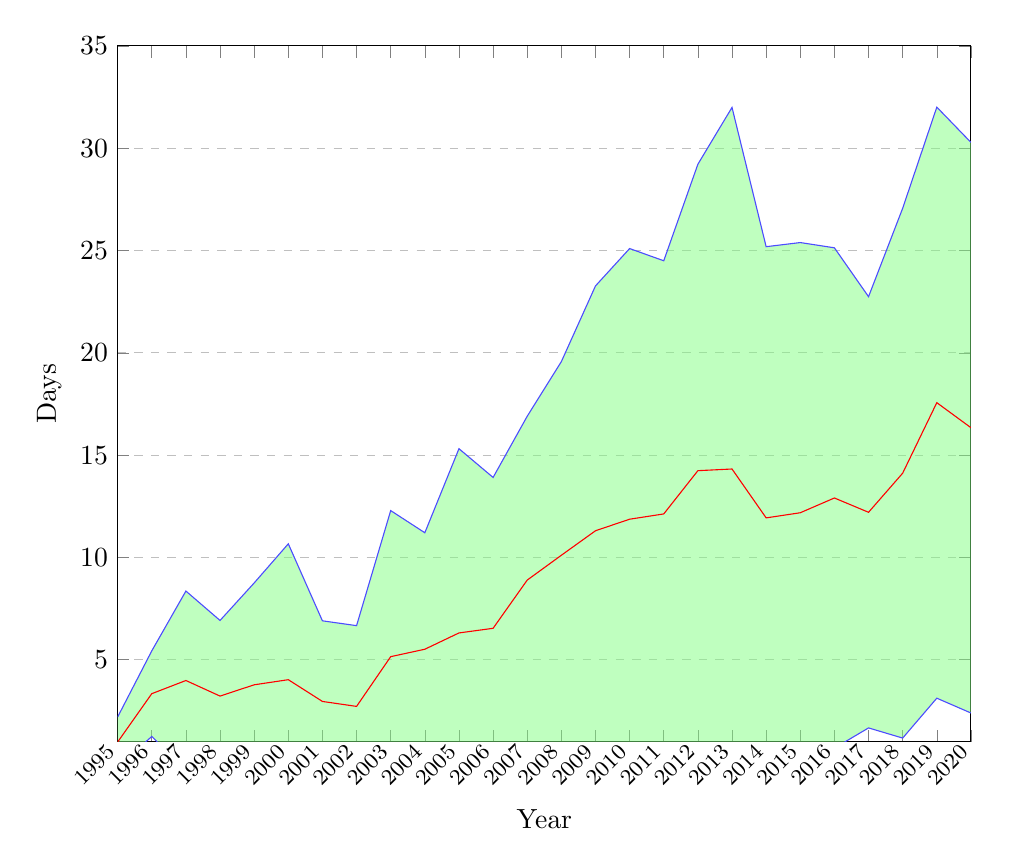
\begin{tikzpicture}
\begin{axis}[
     /pgf/number format/.cd,
     use comma,
    1000 sep={},
    width=7cm, height=6cm, 
    xlabel={Year},
    ylabel={Days},
    scale=2,
    xmin=1995, xmax=2020,
    ymin=1, ymax=35,
    xtick={1990,1991,1992,1993 ,1994,1995,1996,1997,1998,1999,2000,2001,2002,2003,2004,2005,2006,2007,2008,2009,2010,2011,2012,2013,2014,2015,2016,2017,2018,2019,2020},
    x tick label style={font=\footnotesize,rotate=45, anchor=east},
    legend pos=north west,
    ymajorgrids=true,
    grid style=dashed,
]


\addplot[color=red] coordinates {
(1995,0.979748185685686)
(1996,3.3429012345679014)
(1997,3.9866254516711828)
(1998,3.225154299672601)
(1999,3.776405873066553)
(2000,4.02591916483315)
(2001,2.9634600215263034)
(2002,2.7208327974965703)
(2003,5.151680933235868)
(2004,5.51441265587782)
(2005,6.310517238834918)
(2006,6.537172986478542)
(2007,8.893092615857064)
(2008,10.10630700420954)
(2009,11.303461541734748)
(2010,11.868171806917212)
(2011,12.125650036251587)
(2012,14.239504293801572)
(2013,14.321117469607993)
(2014,11.932393414500448)
(2015,12.183628837945754)
(2016,12.904897473384315)
(2017,12.205768003481724)
(2018,14.117222824341681)
(2019,17.562622253086417)
(2020,16.339489975512706)
};


\addplot[name path=us_top,color=blue!70] coordinates {
(1995,2.2033788316755683)
(1996,5.433947810341324)
(1997,8.357325582812347)
(1998,6.920828842255933)
(1999,8.752969510473655)
(2000,10.665780562896723)
(2001,6.902625960252331)
(2002,6.666968324256853)
(2003,12.289292381692503)
(2004,11.205850706436934)
(2005,15.313024283461473)
(2006,13.90895723049302)
(2007,16.899437725893648)
(2008,19.568548060956722)
(2009,23.26748289945725)
(2010,25.09324839600957)
(2011,24.49638414760995)
(2012,29.213792496827296)
(2013,31.989865070370776)
(2014,25.184240020644204)
(2015,25.386096980499836)
(2016,25.12911097368187)
(2017,22.741616580912556)
(2018,27.061198354857403)
(2019,32.00310826131279)
(2020,30.280693234138326)
};


\addplot[name path=us_down,color=blue!70] coordinates {
(1995,-0.24388246030419625)
(1996,1.2518546587944792)
(1997,-0.3840746794699821)
(1998,-0.4705202429107307)
(1999,-1.200157764340548)
(2000,-2.613942233230423)
(2001,-0.9757059171997242)
(2002,-1.225302729263713)
(2003,-1.9859305152207671)
(2004,-0.1770253946812952)
(2005,-2.6919898057916383)
(2006,-0.8346112575359337)
(2007,0.8867475058204803)
(2008,0.6440659474623587)
(2009,-0.6605598159877513)
(2010,-1.356904782175146)
(2011,-0.2450840751067762)
(2012,-0.7347839092241522)
(2013,-3.347630131154789)
(2014,-1.3194531916433103)
(2015,-1.0188393046083295)
(2016,0.6806839730867598)
(2017,1.6699194260508907)
(2018,1.1732472938259608)
(2019,3.1221362448600463)
(2020,2.398286716887087)
};






\addplot[green!50,fill opacity=0.5] fill between[of=us_top and us_down];
  
    
\end{axis}
\end{tikzpicture}
\caption{Average duration of a conversation in days }
\end{figure}


\begin{figure}[H]
\hspace*{-0.5cm}
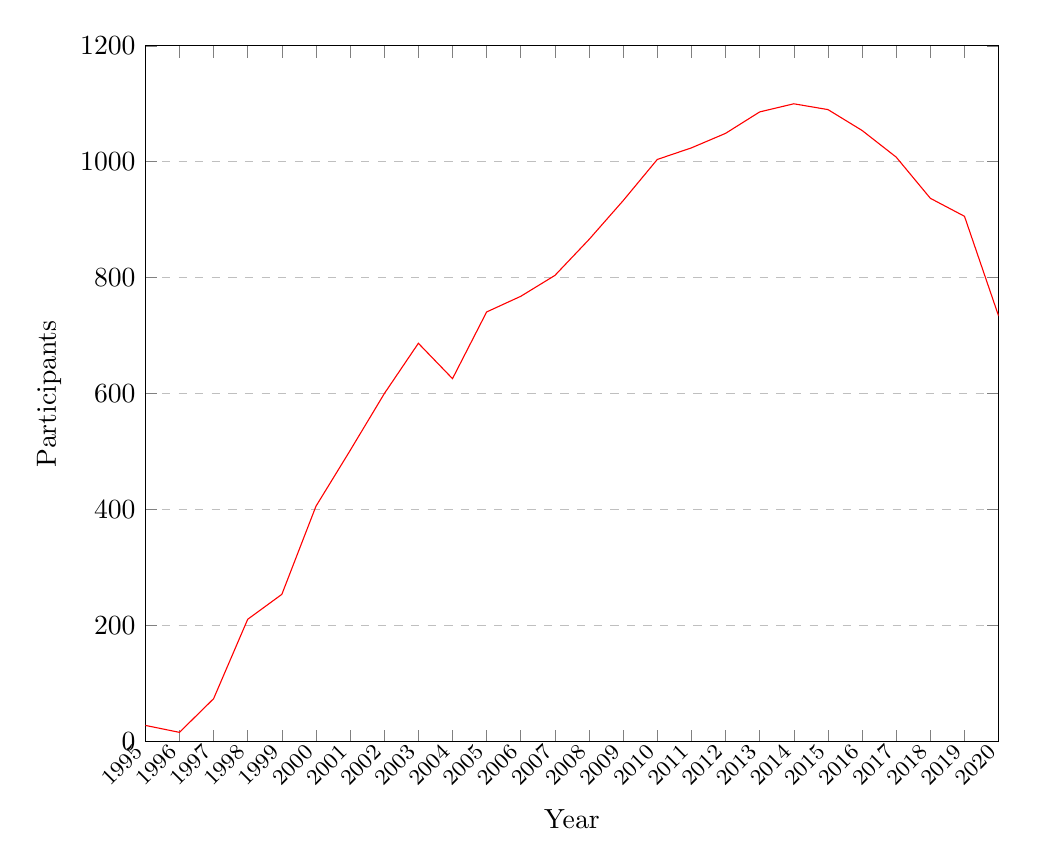
\begin{tikzpicture}
\begin{axis}[
     /pgf/number format/.cd,
     use comma,
    1000 sep={},
    width=7cm, height=6cm, 
    xlabel={Year},
    ylabel={Participants},
    scale=2,
    xmin=1995, xmax=2020,
    ymin=0, ymax=1200,
    xtick={1990,1991,1992,1993 ,1994,1995,1996,1997,1998,1999,2000,2001,2002,2003,2004,2005,2006,2007,2008,2009,2010,2011,2012,2013,2014,2015,2016,2017,2018,2019,2020},
    x tick label style={font=\footnotesize,rotate=45, anchor=east},
    legend pos=north west,
    ymajorgrids=true,
    grid style=dashed,
]

\addplot[color=red] coordinates {
(1995,28)
(1996,16)
(1997,74)
(1998,211)
(1999,254)
(2000,406)
(2001,502)
(2002,600)
(2003,687)
(2004,626)
(2005,741)
(2006,768)
(2007,804)
(2008,866)
(2009,933)
(2010,1004)
(2011,1024)
(2012,1049)
(2013,1086)
(2014,1100)
(2015,1090)
(2016,1054)
(2017,1008)
(2018,937)
(2019,906)
(2020,734)
};



    
\end{axis}
\end{tikzpicture}
\caption{Amount of participants in conversations containing the “last call” phrase.}
\end{figure}



Something to note about this graph is how the length of the “last call” thread has been steadily increasing from the very beginning. This could be for several reasons, in the early days, as previously noted, not everything was archived,  meaning the threads, if any, would naturally be shorter. In fact, no threads before the year 1995 were even found.
As the archiving developed, more and more messages were properly archived, and the length naturally increased. This however only applies to the very early messages, and does not in itself explain why the length kept increasing.\\

The reason could be that as time goes by, and RFCs are made to either update old RFCs, or to define entirely new standards, their complexity increases. This would in turn increase the amount of work and time that has to be put into creating them, resulting in longer threads. \\

The steady increase in participants also likely contributed to the increased length of threads.
In fact, in figure 7.5 we can see that the amount of participants started to decline in 2014, figure 7.6 shows a decrease in thread duration at that time as well. The thread duration did recover around 2017 however, while the amount of participants continued to decline. This means that the remaining people are doing more work now than ever (possibly due to Covid-19), or that there is not as much work to be done as there was in the previous years.




\chapter{Connecting RFC authors to the email archives}


In order to gain a better understanding of how exactly a person contributes to the IETF, both by authoring RFCs, and partaking in discussion, we first need get a better grasp on what exactly a person is, in the context of this project. Recall the documents files from chapter 5.
Several of them were specifically designed to contain the names that were found with their corresponding email address. And while these are now readily available and ready to be used, they are not necessarily a good representation of a person.

First of all, a way to determine a person exactly, or at the very least with a high probability, is needed. One set of names that are one hundred percent guaranteed to not only be actual people, but also active members of the IETF that have already contributed to the organization, are authors of RFCs.  

A .bib file for citing RFCs has been created by Dr.-Ing. Roland Bless.
This file contains not only the names of authors, but the date of publication as well, which can be used to bind RFC publications closed to conversation threads.
The .bib file can be found at the following address.\\

\url{https://tm.uka.de/~bless/bibrfcindex.html}\\

This file not only makes it possible to cite RFCs in LaTeX, it is also a very well structured file that can be parsed into Solr for easy access.
Doing this makes it possible to search for RFCs in Solr in the same way as the email archives. It makes it possible, for example, to compare email activity in the archives to the amount of RFCs published in the same timeframe.
This again will make it possible to check if a conversation thread ends in an RFC publication.

The names of authors in RFCs are also very well structured, unlike what we find in the email archives. In the RFC documents, the name of the author, or authors, is always abbreviated, with the exception of their last name.

This however, is a problem, as a person's last names and initials are simply not good enough to identify them, at least not on the global scale this project is working on. Common names like “Kowalski”, “Ødegård” and similar are very likely to appear far more frequently than others, and authors with these last names would most likely be swallowed up in a sea of others with the same name. In fact, only about 55\% of all authors can be correctly identified by using this method. And last but not least, the .bib file does not contain any information regarding the email addresses of authors.

In conclusion, the data found in the .bib file is not sufficient for establishing a connection between the RFC authors and their messages in the email archives.

\section{IETF Datatracker}



In contrast to the .bib files, the RFC documents found in the IETF datatracker contain not only full names of the authors, but sometimes their email addresses as well. However, yet again, in contrast to the .bib file and the email archives, there is not an easy way to extract this information.\\

Two different approaches to obtaining this data were considered for this project:\\


\emph{Approach 1:}\\
The first approach is essentially the same way that was used to download the email archives. Make a program that would automatically download all of the RFC pages, then parse them in order to obtain the desired data.\\\\

\emph{Approach 2:} \\
Scrape data directly from the page by using a Python module with such functionality.\\

For this project, the second approach was used as it ensures that the extracted data is always up to date, as well as saving on storage space and file seek overhead. 



\subsection{The web scraper}
The scraper was developed with the help of the “BeautifulSoup” Python module. The high level description of this program is as follows:

\begin{enumerate}

\item Connect to the specified url.\\
 This is simple to do as the urls follows a very simple format like so:\\
\url{https://datatracker.ietf.org/doc/rfc0000/}\\

One can simply start at 0 and iterate over all addresses by increasing the RFC id counter by 1 each time. If the RFC with a given id does not exist, the connection attempt will fail, and the exception has to caught. 



\item By using the previously mentioned module, parse the page, and look for a “href” attribute that starts with “/person/”. This attribute specifically holds the email address of a person. In some cases, the email address is simply not there. In those cases, the name of the author is contained within this attribute instead. These cases are easy to distinguish, as a person's name always consists of at least two strings separated by a space. The way html encodes spaces is by replacing them with a “\%20”, this means that if a string obtained from the “href” attribute contains said substring, it is not an email address, and can be ignored. 

\item The previously mentioned href attribute is always followed by a “span class” attribute, with no name, again with the help of the beautifulsoup module, this attribute can be retrieved.


\end{enumerate}

\subsection{Further data extraction}

Now that there exists a concrete set of name and address pairs that are guaranteed to belong to actual individuals, it is possible to use the email archives to extract even more data about them. 
Firstly, a single email address per name may not tell the entire story, people tend to change their email address for a wide variety of reasons, like changing workplace or their position at the company. This means that in order to get all messages sent by a specific person, all of those email addresses are needed.
The same goes for names, it is not impossible for a person to change their name. It is not unusual to change your last name when getting married for example.\\

This overall means that the definition of a person needs to be adjusted to account for these facts. Up until now the unspoken assumption about “people” was that they are uniquely identified by their name and email address pair. This no longer holds if more addresses or name changes are introduced into the mix.

For this reason, a person was assigned an id that uniquely identifies them.\\

But how does one go about finding the previously mentioned email addresses?
The answer to this question depends on what is chosen to identify a person in the email database, versus the people obtained by scraping the IETF datatracker. \\

Essentially, if one assumes that the names found in the datatracker are unique identifiers, then the email archives can be used to obtain other email addresses a person has used, given they signed their emails with their actual name.
Similarly, if we assume that an email address uniquely identifies a person, any other names a person may have used, can be found.

Both of these approaches involve some risks. For example, given the second assumption, if a name is ever used in conjunction with a “shared” email address, the names of all other people to have ever used said address would all be regarded as one. One of the previously blacklisted email addresses, for example "notifications@github.com" is such an address.

One way of avoiding this, aside from manually blacklisting said address, could be to arbitrarily limit the amount of names that can be associated with an address. While this is strictly speaking not a very scientific solution, it should at the very least remove the most contested email addresses.

For this reason, a list of the top 40 most contested email addresses was created and curated by hand to serve as a blacklist.    
The entire list can be found below.\\


\begin{center}
 \begin{tabular}{||c | c||} 
 \hline
 \textit{Address} & \textit{Amount of names} \\ [1ex] 
 \hline\hline

notifications@github.com & 536\\
\hline

noreply@ietf.org & 540\\
\hline

atompub-archive@megatron.ietf.org & 452\\
\hline

aaa-archive@lists.ietf.org & 320\\
\hline

eap-archive@megatron.ietf.org & 500\\
\hline

calsch-archive@ietf.org & 560\\
\hline

kink-archive@lists.ietf.org & 432\\
\hline

ecm-archive@ietf.org & 296\\
\hline

calsch-archive@megatron.ietf.org & 208\\
\hline

cdi-archive@ietf.org & 448\\
\hline

drums-archive@ietf.org & 398\\
\hline

eap-archive@ietf.org & 336\\
\hline

ldapbis-archive@megatron.ietf.org & 578\\
\hline

dnsext-archive@ietf.org & 324\\
\hline

capwap-archive@ietf.org & 504\\
\hline

aaa-archive@ietf.org & 348\\
\hline

ediint-archive@ietf.org & 302\\
\hline

ldapbis-archive@lists.ietf.org & 738\\
\hline

frnetmib-archive@ietf.org & 270\\
\hline

conneg-archive@ietf.org & 390\\
\hline

aft-archive@ietf.org & 276\\
\hline

ipdvb-archive@megatron.ietf.org & 206\\
\hline

rescap-archive@ietf.org & 278\\
\hline

kink-archive@ietf.org & 250\\
\hline

calsch-archive@lists.ietf.org & 268\\
\hline

rsvp-archive@lists.ietf.org & 380\\
\hline

v6ops-archive@ietf.org & 216\\
\hline

ipdvb-archive@ietf.org & 294\\
\hline

web-archive@ietf.org & 224\\
\hline

webdav-archive@ietf.org & 218\\
\hline

dnsind-archive@ietf.org & 276\\
\hline

eos-archive@ietf.org & 364\\
\hline

ipvbi-archive@ietf.org & 208\\
\hline

weird-archive@ietf.org & 236\\
\hline

issll-archive@lists.ietf.org & 352\\
\hline

idmr-archive@ietf.org & 216\\
\hline

ipp-archive@megatron.ietf.org & 204\\
\hline

provreg-archive@ietf.org & 218\\
\hline

tcpsat-archive@ietf.org & 232\\
\hline

16ng@ietf.org & 212\\
\hline


\end{tabular}
\end{center}

A similar situation takes place with the first assumption. Simply put, if the assumption does not hold, and there is a name  overlap between several authors in the IETF datatracker, a lot of unrelated email addresses will end up being assigned to one name.

An arbitrary limit on how many different email addresses a name may belong to may be set. In addition, a limit on edit distance from any of the already known email addresses may be set in order to improve results. 

Despite this, the assumption of names of RFC authors being unique identifiers was made. This was done since the probability of two people having the exact string as their name is very low given the number of RFC authors.
This allowed to retrieve a more complete set of addresses.\\ 



Connecting threads to RFCs can be done in several ways. In order to be able to link RFC to threads, one needs to know when any given RFC was published. One way of obtaining this information could be, scraping this information from the IETF datatracker. This is not possible however, as the date present in the datatracker, is the “last updated” date, not the date of publication. 
In RFC 822 \cite{RFC0822} for example, this date is set to 9. of July 2020, which is clearly not the publication date. There is another way, the previously mentioned .bib file, does in fact contain the proper publication dates. The only downside to using this .bib file is the fact that the dates contained within do not specify the day of publication, only the year and month. This should still be sufficient in tracing down which RFCs were published around the time a conversation thread took place. In order to make this data easily accessible a new Solr core was created, and a simple parser for the .bib file was developed. This core contains only very simple documents with only five fields each, the date of publication, the RFC identifier, the title, the working group name, and the name of the author.

In order to get the best possible results, both the .bib file and the scraper used previously were combined and used to create the documents. The .bib file was used as a way to keep track of RFC identifiers, as well as their publication date, and the datatracker was used to retrieve names and email addresses, like it did previously. 

The same program is also responsible for extracting a more complete set of addresses. This is done due to the amount of time it takes to scrape all the required information from the web, and as the full names of authors are needed in both cases, it was seen as a good idea to kill two birds with one stone.  

The outline of the program is as follows.

\begin{itemize}

\item Parse the .bib file, obtain a list of RFC that can later be used to create the appropriate url for the web scraper. Extract the date.
\item For each RFC in the .bib file, use the scraper to obtain the name of the author. At this point, the documents are ready to be uploaded to Solr.


\item For each name extracted from the IETF datatracker, look up email addresses associated with that name. Depending on what option was chosen, either filter the results using the previously presented black list, or see how many names are associated with any address in the results, and remove those that do not meet the requirements.



\end{itemize}


The results of this program were yet again uploaded to Solr, to two new cores respectively named “authors” and “rfc”. With these two in place it became possible to link messages sent by any given RFC author, to messages they have sent around at that time.\\


The schemas for the non-standard fields in these cores can be found below.\\

\textbf{The "author" core schema:}
\begin{center}
 \begin{tabular}{||c | c||} 
 \hline
 \textit{Field name} & \textit{Tokenizer} \\ [1ex] 
 \hline\hline


name & solr.KeywordTokenizerFactory\\

\hline

address & solr.KeywordTokenizerFactory\\

\hline

wg & solr.KeywordTokenizerFactory\\

\hline



\end{tabular}
\end{center}


\textbf{The "rfc" core schema:}
\begin{center}
 \begin{tabular}{||c | c||} 
 \hline
 \textit{Field name} & \textit{Tokenizer} \\ [1ex] 
 \hline\hline


date & No tokenizer\\

\hline


number & No tokenizer\\

\hline


author & solr.KeywordTokenizerFactory\\

\hline



title & solr.StandardTokenizerFactory\\

\hline


wg & solr.KeywordTokenizerFactory\\

\hline


\end{tabular}
\end{center}


\subsection{The code}

As described earlier, the first step of the program is to read the .bib file. 
This file contains a given amount of “structures” representing information regarding an RFC. This format can be seen below:




\lstinputlisting[showstringspaces=false,language=Python,firstline=0, lastline=18]{rfc_bib.bib}


This is easily done as it is a very well structured file. It has a downside however: many of the “fields” in said file all contain the same information, and not all fields are interesting either.
The only fields that are relevant to this project are:

\begin{itemize}

\item Author
\item Title
\item Year

\end{itemize}

Strictly speaking, the title of the RFC is not necessary, but has been added as it may prove useful in the future.

\subsubsection{Part 1, parsing the .bib file}

An attempt at splitting each line of the .bib file using a “=” as the delimiter is made in order to split the line into two components, its field name, and the data contained within. The first element of this list is always assumed to be the fields name.\\

The first element still need its preceding whitespace removed before it can be properly matched. The removal of this whitespace is done by the “strip()” method.\\

The first field the program looks for is the “author” field, as this is the field that always precedes any other fields in the .bib file.
This field always contains one or more names, which are, as previously described, just the author's initials followed by their last name. If there is more than one name in this field, they will always be separated by an “and”, this means that it is easy to parse this field into a list, by using the “split()” method and using “  and ” as the delimiter.\\


\lstinputlisting[showstringspaces=false,language=Python,firstline=47, lastline=61]{parser.py}

The next step depends on whether the split actually split the string to several parts. If it did not, the first character of the name string will have a quotation sign at the start, as well as a newline, a comma, and another quotation mark at the end. These are easily removed by slicing the string.
This is a bit more complicated if there are 2 or more names.
The first one will always begin with a quotation mark, and the last one with a newline, a comma and a quotation mark, which are again removed by slicing the respective strings. Any string located between the start and end of the list do not need any further processing: 


\lstinputlisting[showstringspaces=false,language=Python,firstline=62, lastline=75]{parser.py}

The next two fields,”number” and “title”, do not need much processing aside from slicing away the character at the beginning and at the end:

\lstinputlisting[showstringspaces=false,language=Python,firstline=78, lastline=90]{parser.py}

The last remaining field, namely “date”, needs to be converted into the Solr format, the fact that these dates only describe the year and month of publication is taken care of during the conversion. The program slices up the string into its two components, the year and the month. Since the month field in the .bib file does not contain the numeric representation, but a text based one, it needs to be converted into a numeric one in order to meet the Solr format. This is done by the “getMonth()” method, that is essentially just a series of “if” checks. 
Since there is no day, hours, or minutes in the .bib file, the day has been set to the first one, and the time has been set to 0 hours, 0 minutes, and 0 seconds. This needs to be taken into consideration when linking RFC publications to dates found in the main database core, as the dates in the documents produced by this parser are better described as “month long periods of time” rather than exact dates:

\lstinputlisting[showstringspaces=false,language=Python,firstline=98, lastline=106]{parser.py}

\subsubsection{Part 2, scraping the IETF datatracker}

Now that the .bib file is fully parsed and loaded, the next step is to scrape data from IETF datatracker by using the previously mentioned Beautifulsoup module. 
This part of the program makes use of the parsed .bib file to keep track of existing RFC numbers.
As this part of the program is connected to a remote address, there is always a chance that said attempt may fail. In this case, the extraction fails. This was not an option in this case, only a perfect result would be satisfactory. For this reason, the program is made to retry as many times as needed. This is dangerous to do however, as it is absolutely possible that the attempt never actually succeeds, resulting in an endless loop. This could be easily prevented by setting a certain number of times the program is allowed to retry it. Despite this, said solution was not used, and the program did terminate, and successfully scraped all requested data.\\  
\smallskip
\lstinputlisting[showstringspaces=false,language=Python,firstline=120, lastline=124]{parser.py}
\smallskip
First, the program opens a connection to the specified url, and the contents are parsed by the Beautifulsoup module:  \\
\smallskip
\lstinputlisting[showstringspaces=false,language=Python,firstline=127, lastline=129, breaklines=true]{parser.py}
\medskip
Next a list of all href attributes is made. In this list, the elements that start with “/person/” is the one containing the email addresses of the authors. These are added to a list.\\
\smallskip
\lstinputlisting[showstringspaces=false,language=Python,firstline=135, lastline=137]{parser.py}
\smallskip

In order to retrieve the names, a list of all classes is retrieved. Curiously, the class with no name is the one containing the names of the authors. One thing to note here, is that the names and addresses always come in the same order. The first address found, will always belong to the first name found.\\

\smallskip
\lstinputlisting[showstringspaces=false,language=Python,firstline=141, lastline=143]{parser.py}
\smallskip

The name retrieval can “fail” in a sense: simply, if there is no name to be found, the string “Unknown” will be in its place. If this is not the case, the names retrieved from the datatracker are used to replace the names of authors retrieved from the .bib file in their respective RFC: 
\smallskip
\lstinputlisting[showstringspaces=false,language=Python,firstline=145, lastline=146]{parser.py}
\smallskip
Finally, if any addresses were retrieved, the name and address are stored for later use. This also means that authors who did not have any address associated with them, will be absent from the author database. This mainly applies to the RFCs from one to one thousand.
For example, the author of RFC~1 \cite{RFC0001}, according to the .bib file is “S. Crocker”, as there is no address to this name in the IETF datatracker, said author is absent from the author database. 

\smallskip
\lstinputlisting[showstringspaces=false,language=Python,firstline=152, lastline=158]{parser.py}
\smallskip

The working group of an RFC is extracted in a similar manner.


\lstinputlisting[showstringspaces=false,language=Python,firstline=145, lastline=149]{web_crawler_v2.py}

At the very end, the “retry” variable is set to “False” in order to break the loop.


\subsubsection{Part 3, further data extraction}


The last part of the program is responsible for extracting a more complete set of email addresses for the authors. As such, the program begins by establishing a connection to the mail database core, where this information resides. Next the complete blacklist is loaded and the extraction process begins. 
The extraction process is simple yet has some unfortunate quirks. In order to retrieve more email adresses one must first search for all documents with the author's name in the “From-name” field. As one may recall from chapter 4, this is a multivalued field. This means that the faced function cannot be used, as documents with more than one value in this field would return all of their value as the result. This would mean addresses that do not belong to the authors, would be assigned to them anyway. One way of avoiding this is only taking messages with one singular value in this field into consideration. Unfortunately, the version of Solr used for this project does not support queries based on the amount of values in the multivalued field. This leaves only one option: making the program check the length by itself. This however means that the entire results set needs to be checked. This is significantly slower than using the facet function, but is the only way to get the desired results. The “fl” parameter has been set to the “From-address” field in order to speed up the process.

\lstinputlisting[showstringspaces=false,language=Python,firstline=175, lastline=202, breaklines=true]{parser.py}

The results this program produces are finally uploaded to their respective Solr cores, those being named “authors” and “rfc”.
\subsection{Statistics}


With these two cores in place it is now possible not only to link authors to their sent messages, but also to extract statistics regarding the authors. Here is just some of the information that can be extracted from these two cores.\\

The following table shows the 10 most active authors, that is, the authors that have their names listed in the largest number of RFCs.



\begin{center}
\begin{table}
\centering
 \begin{tabular}{||c | c | c||} 
 \hline
\textit{Ranking} & \textit{Name} & \textit{RFC count} \\ [1ex] 
 \hline\hline
1 & Russ Housley & 96\\
\hline

2 & Donald Eastlake & 95\\
\hline

3 & Keith McCloghrie & 92\\
\hline

4 & Henning Schulzrinne & 90\\
\hline

5 & Hannes Tschofenig & 85\\
\hline

6 & Yakov Rekhter & 78\\
\hline

7 & Jonathan Rosenberg & 72\\
\hline

8 & Adrian Farrel & 71\\
\hline

9 & Paul Hoffman & 70\\
\hline

10 & Gonzalo Camarillo & 70\\
\hline

11 & Marshall Rose & 65\\
\hline

12 & Fred Baker & 65\\
\hline

13 & Alexey Melnikov & 60\\
\hline

14 & John Klensin & 59\\
\hline

15 & Mohamed Boucadair & 54\\
\hline

16 & Eric Rosen & 54\\
\hline

17 & Dave Thaler & 54\\
\hline

18 & Brian Carpenter & 54\\
\hline

19 & Bernard Aboba & 54\\
\hline

20 & Carlos Pignataro & 52\\
\hline


\end{tabular}

\caption{Top 20 authors of RFCs.}
\end{table}
\end{center}


\begin{figure}[H]
\hspace*{-0.5cm}
\centering
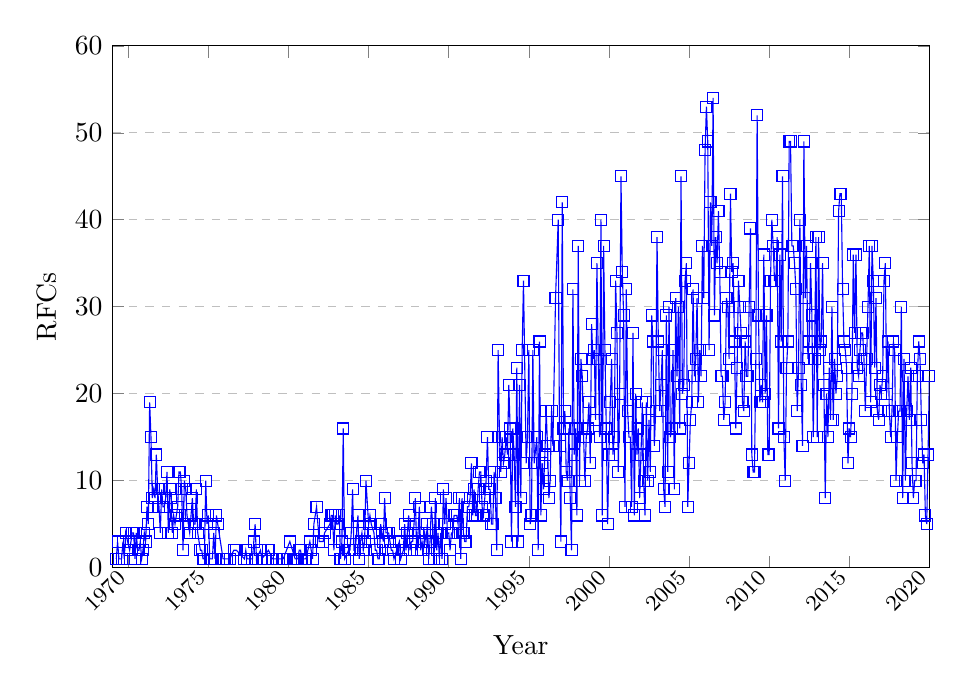
\begin{tikzpicture}
\begin{axis}[
     /pgf/number format/.cd,
     use comma,
    1000 sep={},
    width=8.5cm, height=6cm, 
    xlabel={Year},
    ylabel={RFCs},
    scale=1.5,
    xmin=1969, xmax=2020,
    ymin=0, ymax=60,
    x tick label style={font=\footnotesize,rotate=45, anchor=east},
    legend pos=north west,
    ymajorgrids=true,
    grid style=dashed,
]


\addplot[
    color=blue,
    mark=square,
    ]
    coordinates {
((1969.25,1)(1969.3333333333333,3)(1969.4166666666667,1)(1969.5833333333333,1)(1969.6666666666667,3)(1969.75,1)(1969.8333333333333,4)(1970.0833333333333,2)(1970.1666666666667,3)(1970.25,4)(1970.3333333333333,4)(1970.4166666666667,1)(1970.5,4)(1970.5833333333333,2)(1970.6666666666667,2)(1970.75,3)(1970.8333333333333,1)(1970.9166666666667,2)(1971.0,4)(1971.0833333333333,3)(1971.1666666666667,7)(1971.25,5)(1971.3333333333333,19)(1971.4166666666667,15)(1971.5,8)(1971.5833333333333,9)(1971.6666666666667,8)(1971.75,13)(1971.8333333333333,9)(1971.9166666666667,7)(1972.0,4)(1972.0833333333333,9)(1972.1666666666667,7)(1972.25,7)(1972.3333333333333,8)(1972.4166666666667,11)(1972.5,4)(1972.5833333333333,9)(1972.6666666666667,8)(1972.75,4)(1972.8333333333333,6)(1972.9166666666667,5)(1973.0,6)(1973.0833333333333,7)(1973.1666666666667,11)(1973.25,11)(1973.3333333333333,9)(1973.4166666666667,2)(1973.5,10)(1973.5833333333333,9)(1973.6666666666667,6)(1973.75,5)(1973.8333333333333,4)(1973.9166666666667,6)(1974.0,8)(1974.0833333333333,5)(1974.1666666666667,5)(1974.25,9)(1974.3333333333333,4)(1974.5,2)(1974.5833333333333,2)(1974.6666666666667,1)(1974.75,1)(1974.8333333333333,10)(1974.9166666666667,5)(1975.0,6)(1975.0833333333333,1)(1975.1666666666667,1)(1975.25,1)(1975.3333333333333,4)(1975.4166666666667,1)(1975.5,6)(1975.5833333333333,5)(1975.9166666666667,1)(1976.0,1)(1976.1666666666667,1)(1976.3333333333333,1)(1976.5833333333333,2)(1976.75,2)(1977.25,1)(1977.3333333333333,2)(1977.4166666666667,1)(1977.75,1)(1977.8333333333333,3)(1977.9166666666667,5)(1978.0,1)(1978.25,2)(1978.3333333333333,1)(1978.75,2)(1979.0,1)(1979.25,1)(1979.4166666666667,1)(1979.5833333333333,1)(1979.6666666666667,1)(1980.0833333333333,3)(1980.4166666666667,1)(1980.5,1)(1980.5833333333333,1)(1980.6666666666667,2)(1980.75,2)(1980.8333333333333,1)(1981.0,1)(1981.0833333333333,1)(1981.3333333333333,3)(1981.4166666666667,2)(1981.5,1)(1981.5833333333333,5)(1981.75,7)(1981.9166666666667,3)(1982.1666666666667,3)(1982.25,4)(1982.5833333333333,5)(1982.6666666666667,6)(1982.75,6)(1982.8333333333333,2)(1982.9166666666667,6)(1983.0,5)(1983.0833333333333,5)(1983.1666666666667,6)(1983.25,1)(1983.3333333333333,3)(1983.4166666666667,16)(1983.5,1)(1983.75,2)(1983.8333333333333,2)(1983.9166666666667,4)(1984.0,9)(1984.0833333333333,2)(1984.1666666666667,2)(1984.3333333333333,6)(1984.4166666666667,1)(1984.5,3)(1984.5833333333333,4)(1984.6666666666667,2)(1984.75,3)(1984.8333333333333,10)(1985.0,5)(1985.0833333333333,6)(1985.1666666666667,5)(1985.3333333333333,4)(1985.4166666666667,2)(1985.5,2)(1985.5833333333333,1)(1985.6666666666667,1)(1985.75,5)(1985.8333333333333,4)(1985.9166666666667,3)(1986.0,8)(1986.0833333333333,4)(1986.1666666666667,4)(1986.25,4)(1986.3333333333333,3)(1986.4166666666667,2)(1986.5,2)(1986.5833333333333,1)(1986.9166666666667,3)(1987.0,1)(1987.1666666666667,2)(1987.25,5)(1987.3333333333333,2)(1987.4166666666667,4)(1987.5,6)(1987.5833333333333,2)(1987.6666666666667,3)(1987.75,3)(1987.8333333333333,5)(1987.9166666666667,8)(1988.0,2)(1988.0833333333333,4)(1988.1666666666667,7)(1988.25,2)(1988.3333333333333,3)(1988.4166666666667,2)(1988.5,4)(1988.5833333333333,3)(1988.6666666666667,5)(1988.75,1)(1988.8333333333333,3)(1988.9166666666667,7)(1989.0,5)(1989.0833333333333,1)(1989.1666666666667,8)(1989.25,2)(1989.3333333333333,4)(1989.4166666666667,1)(1989.5,4)(1989.5833333333333,1)(1989.6666666666667,9)(1989.75,5)(1989.8333333333333,8)(1989.9166666666667,4)(1990.0,4)(1990.0833333333333,2)(1990.1666666666667,4)(1990.25,4)(1990.3333333333333,6)(1990.4166666666667,6)(1990.5,6)(1990.5833333333333,5)(1990.6666666666667,8)(1990.75,1)(1990.8333333333333,8)(1990.9166666666667,4)(1991.0,3)(1991.0833333333333,3)(1991.1666666666667,7)(1991.25,7)(1991.3333333333333,8)(1991.4166666666667,12)(1991.5,6)(1991.5833333333333,9)(1991.6666666666667,6)(1991.75,6)(1991.8333333333333,9)(1991.9166666666667,11)(1992.0,11)(1992.0833333333333,7)(1992.1666666666667,6)(1992.25,8)(1992.3333333333333,10)(1992.4166666666667,15)(1992.5,9)(1992.5833333333333,9)(1992.6666666666667,5)(1992.75,5)(1992.8333333333333,11)(1992.9166666666667,8)(1993.0,2)(1993.0833333333333,25)(1993.1666666666667,15)(1993.25,11)(1993.3333333333333,15)(1993.4166666666667,12)(1993.5,13)(1993.5833333333333,15)(1993.6666666666667,13)(1993.75,21)(1993.8333333333333,16)(1993.9166666666667,3)(1994.0,16)(1994.0833333333333,13)(1994.1666666666667,7)(1994.25,23)(1994.3333333333333,3)(1994.4166666666667,21)(1994.5,8)(1994.5833333333333,25)(1994.6666666666667,33)(1994.8333333333333,12)(1994.9166666666667,15)(1995.0,25)(1995.0833333333333,5)(1995.1666666666667,6)(1995.25,25)(1995.3333333333333,12)(1995.5,15)(1995.5833333333333,2)(1995.6666666666667,26)(1995.75,6)(1995.8333333333333,12)(1995.9166666666667,9)(1996.0,13)(1996.0833333333333,18)(1996.1666666666667,14)(1996.25,8)(1996.3333333333333,10)(1996.4166666666667,18)(1996.5,14)(1996.6666666666667,31)(1996.8333333333333,40)(1996.9166666666667,14)(1997.0,3)(1997.0833333333333,42)(1997.1666666666667,16)(1997.25,18)(1997.3333333333333,11)(1997.4166666666667,10)(1997.5,16)(1997.5833333333333,8)(1997.6666666666667,2)(1997.75,32)(1997.8333333333333,13)(1997.9166666666667,16)(1998.0,6)(1998.0833333333333,37)(1998.1666666666667,10)(1998.25,24)(1998.3333333333333,22)(1998.4166666666667,15)(1998.5,10)(1998.5833333333333,15)(1998.6666666666667,16)(1998.75,19)(1998.8333333333333,12)(1998.9166666666667,28)(1999.0,24)(1999.0833333333333,25)(1999.1666666666667,17)(1999.25,35)(1999.3333333333333,24)(1999.4166666666667,15)(1999.5,40)(1999.5833333333333,6)(1999.6666666666667,37)(1999.75,25)(1999.8333333333333,16)(1999.9166666666667,5)(2000.0,13)(2000.0833333333333,19)(2000.1666666666667,24)(2000.25,13)(2000.3333333333333,15)(2000.4166666666667,33)(2000.5,27)(2000.5833333333333,11)(2000.6666666666667,20)(2000.75,45)(2000.8333333333333,34)(2000.9166666666667,29)(2001.0,7)(2001.0833333333333,32)(2001.1666666666667,18)(2001.25,15)(2001.3333333333333,15)(2001.4166666666667,7)(2001.5,27)(2001.5833333333333,6)(2001.6666666666667,20)(2001.75,13)(2001.8333333333333,16)(2001.9166666666667,8)(2002.0,13)(2002.0833333333333,19)(2002.1666666666667,10)(2002.25,6)(2002.3333333333333,19)(2002.4166666666667,10)(2002.5,17)(2002.5833333333333,11)(2002.6666666666667,29)(2002.75,26)(2002.8333333333333,14)(2002.9166666666667,18)(2003.0,38)(2003.0833333333333,26)(2003.1666666666667,18)(2003.25,21)(2003.3333333333333,25)(2003.4166666666667,9)(2003.5,7)(2003.5833333333333,29)(2003.6666666666667,11)(2003.75,30)(2003.8333333333333,15)(2003.9166666666667,16)(2004.0,25)(2004.0833333333333,9)(2004.1666666666667,31)(2004.25,22)(2004.3333333333333,30)(2004.4166666666667,16)(2004.5,45)(2004.5833333333333,20)(2004.6666666666667,21)(2004.75,33)(2004.8333333333333,35)(2004.9166666666667,7)(2005.0,12)(2005.0833333333333,17)(2005.1666666666667,19)(2005.25,32)(2005.3333333333333,22)(2005.4166666666667,24)(2005.5,31)(2005.5833333333333,19)(2005.6666666666667,25)(2005.75,22)(2005.8333333333333,37)(2005.9166666666667,31)(2006.0,48)(2006.0833333333333,53)(2006.1666666666667,49)(2006.25,25)(2006.3333333333333,42)(2006.4166666666667,37)(2006.5,54)(2006.5833333333333,29)(2006.6666666666667,38)(2006.75,35)(2006.8333333333333,41)(2006.9166666666667,34)(2007.0,22)(2007.0833333333333,22)(2007.1666666666667,17)(2007.25,19)(2007.3333333333333,31)(2007.4166666666667,30)(2007.5,24)(2007.5833333333333,43)(2007.6666666666667,34)(2007.75,35)(2007.8333333333333,26)(2007.9166666666667,16)(2008.0,23)(2008.0833333333333,33)(2008.1666666666667,30)(2008.25,27)(2008.3333333333333,19)(2008.4166666666667,18)(2008.5,26)(2008.5833333333333,22)(2008.6666666666667,22)(2008.75,30)(2008.8333333333333,39)(2008.9166666666667,13)(2009.0,11)(2009.0833333333333,11)(2009.1666666666667,24)(2009.25,52)(2009.3333333333333,29)(2009.4166666666667,19)(2009.5,21)(2009.5833333333333,19)(2009.6666666666667,36)(2009.75,20)(2009.8333333333333,29)(2009.9166666666667,13)(2010.0,13)(2010.0833333333333,33)(2010.1666666666667,40)(2010.25,37)(2010.3333333333333,33)(2010.4166666666667,33)(2010.5,38)(2010.5833333333333,16)(2010.6666666666667,36)(2010.75,26)(2010.8333333333333,45)(2010.9166666666667,15)(2011.0,10)(2011.0833333333333,23)(2011.1666666666667,26)(2011.25,49)(2011.3333333333333,49)(2011.4166666666667,37)(2011.5,37)(2011.5833333333333,35)(2011.6666666666667,32)(2011.75,18)(2011.8333333333333,23)(2011.9166666666667,40)(2012.0,21)(2012.0833333333333,14)(2012.1666666666667,49)(2012.25,31)(2012.3333333333333,37)(2012.4166666666667,24)(2012.5,26)(2012.5833333333333,35)(2012.6666666666667,29)(2012.75,15)(2012.8333333333333,24)(2012.9166666666667,38)(2013.0,15)(2013.0833333333333,38)(2013.1666666666667,25)(2013.25,26)(2013.3333333333333,35)(2013.4166666666667,21)(2013.5,8)(2013.5833333333333,20)(2013.6666666666667,15)(2013.75,23)(2013.8333333333333,17)(2013.9166666666667,30)(2014.0,17)(2014.0833333333333,24)(2014.1666666666667,20)(2014.25,22)(2014.3333333333333,41)(2014.4166666666667,43)(2014.5,43)(2014.5833333333333,32)(2014.6666666666667,26)(2014.75,25)(2014.8333333333333,23)(2014.9166666666667,12)(2015.0,16)(2015.0833333333333,15)(2015.1666666666667,20)(2015.25,36)(2015.3333333333333,27)(2015.4166666666667,36)(2015.5,23)(2015.5833333333333,22)(2015.6666666666667,25)(2015.75,27)(2015.8333333333333,27)(2015.9166666666667,24)(2016.0,18)(2016.0833333333333,24)(2016.1666666666667,30)(2016.25,37)(2016.3333333333333,19)(2016.4166666666667,37)(2016.5,33)(2016.5833333333333,23)(2016.6666666666667,31)(2016.75,18)(2016.8333333333333,17)(2016.9166666666667,21)(2017.0,20)(2017.0833333333333,22)(2017.1666666666667,33)(2017.25,35)(2017.3333333333333,20)(2017.4166666666667,26)(2017.5,18)(2017.5833333333333,15)(2017.6666666666667,18)(2017.75,26)(2017.8333333333333,25)(2017.9166666666667,10)(2018.0,15)(2018.0833333333333,18)(2018.1666666666667,18)(2018.25,30)(2018.3333333333333,8)(2018.4166666666667,24)(2018.5,10)(2018.5833333333333,18)(2018.6666666666667,22)(2018.75,17)(2018.8333333333333,23)(2018.9166666666667,12)(2019.0,8)(2019.0833333333333,10)(2019.1666666666667,10)(2019.25,22)(2019.3333333333333,26)(2019.4166666666667,24)(2019.5,17)(2019.5833333333333,12)(2019.6666666666667,13)(2019.75,6)(2019.8333333333333,5)(2019.9166666666667,13)(2020.0,22)(2020.0833333333333,8)(2020.1666666666667,40)(2020.25,22)(2020.3333333333333,13)(2020.4166666666667,6)(2020.5,15)(2020.5833333333333,10)(2020.6666666666667,21)(2020.75,22)
    };
    
\end{axis}
\end{tikzpicture}
\caption{RFCs published.}
\end{figure}



What about email activity? It would seem natural that more messages are sent by the authors leading up the publication of a new RFC. As previously discussed, RFC publications can only be tracked on a monthly basis. This is not a problem for Solr however, as it is easily able to search for documents contained within a period of time. Since RFCs can only be tracked in this way, the amount of emails sent by authors will also be tracked on a monthly basis.\\\\  

What about author involvement? Are authors the main participants in discussions or do they just create the RFC documents, without participating much in the discussions themselves ?
To answer this question several cases were investigated. 
The graph below shows how many of the top one hundred posters each year were authors. 
The percentage was calculated on a per-address basis. This means that if an author, as defined in the “author” core, used several of his email addresses in a given year, they would be counted several times. 






\begin{figure}[H]
\hspace*{-1cm}
\centering
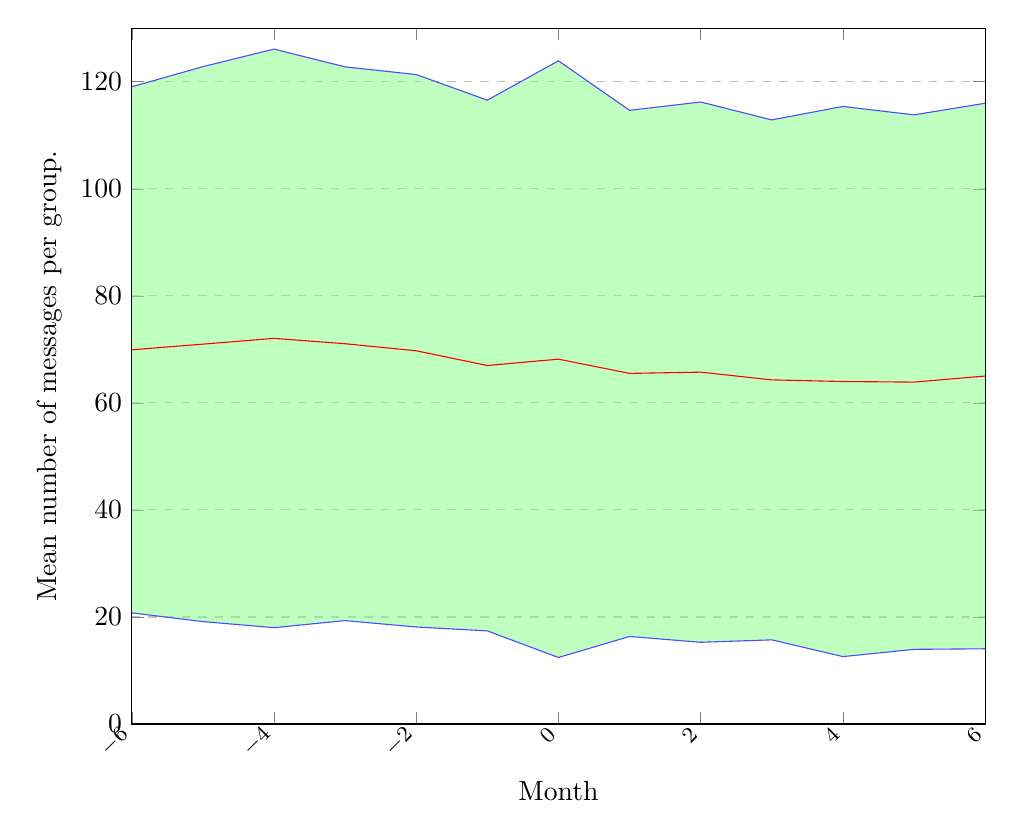
\begin{tikzpicture}
\begin{axis}[
     /pgf/number format/.cd,
     use comma,
    1000 sep={},
    width=7cm, height=6cm, 
    xlabel={Month},
    ylabel={Mean number of messages per group.},
    scale=2,
    xmin=-6, xmax=6,
    ymin=0, ymax=130,
    x tick label style={font=\footnotesize,rotate=45, anchor=east},
    legend pos=north west,
    ymajorgrids=true,
    grid style=dashed,
]
\addplot[color=red] coordinates {
(-6,69.91586692258477)
(-5,70.97632757517594)
(-4,72.05438259756878)
(-3,71.0505438259757)
(-2,69.73800383877159)
(-1,66.98048624440179)
(+0,68.17082533589252)
(+1,65.51023672424824)
(+2,65.74216250799743)
(+3,64.29942418426104)
(+4,63.99264235444658)
(+5,63.882917466410746)
(+6,65.01951375559821)


};
\addplot[name path=us_top,color=blue!70] coordinates {
(-6,119.06096467238625)
(-5,122.815533614705)
(-4,126.10300200041459)
(-3,122.77673341640836)
(-2,121.3438234971423)
(-1,116.55713109643006)
(+0,123.90766442699503)
(+1,114.65750550395629)
(+2,116.2128439175078)
(+3,112.87031852385972)
(+4,115.3849220587923)
(+5,113.81088793495856)
(+6,115.97989206583513)


};
\addplot[name path=us_down,color=blue!70] coordinates {
(-6,20.77076917278329)
(-5,19.137121535646884)
(-4,18.005763194722967)
(-3,19.324354235543026)
(-2,18.13218418040089)
(-1,17.403841392373515)
(+0,12.433986244790006)
(+1,16.362967944540202)
(+2,15.271481098487072)
(+3,15.728529844662361)
(+4,12.600362650100863)
(+5,13.954946997862933)
(+6,14.059135445361292)


};

\addplot[green!50,fill opacity=0.5] fill between[of=us_top and us_down];
  
    
\end{axis}
\end{tikzpicture}
\caption{Amount of messages sent in a working group, around the time of publication of an RFC from that group. The shaded area indicates the standard deviation.}
\end{figure}

One thing to keep in mind about this graph, as well as all that follows, is that not all working group names from the RFC match up with names of mailing lists in the email archives, and for this reason cannot be linked. This means that roughly one third of all mailing lists found in RFCs are not represented in the graphs. For a full list of said working groups, see the github repository.

The graph above depicts the average email activity in a working group around the time of a RFC publication from that group. The data show clearly that there is essentially no change in email activity, around a publication. A possible reason for this is the fact that RFCs need to be approved by the RFC editor before they can be published. This is usually a quite lengthy process, meaning the working group is usually done with  their discussion by the time the RFC is actually published. 






\begin{figure}[H]
\hspace*{-0.5cm}
\centering
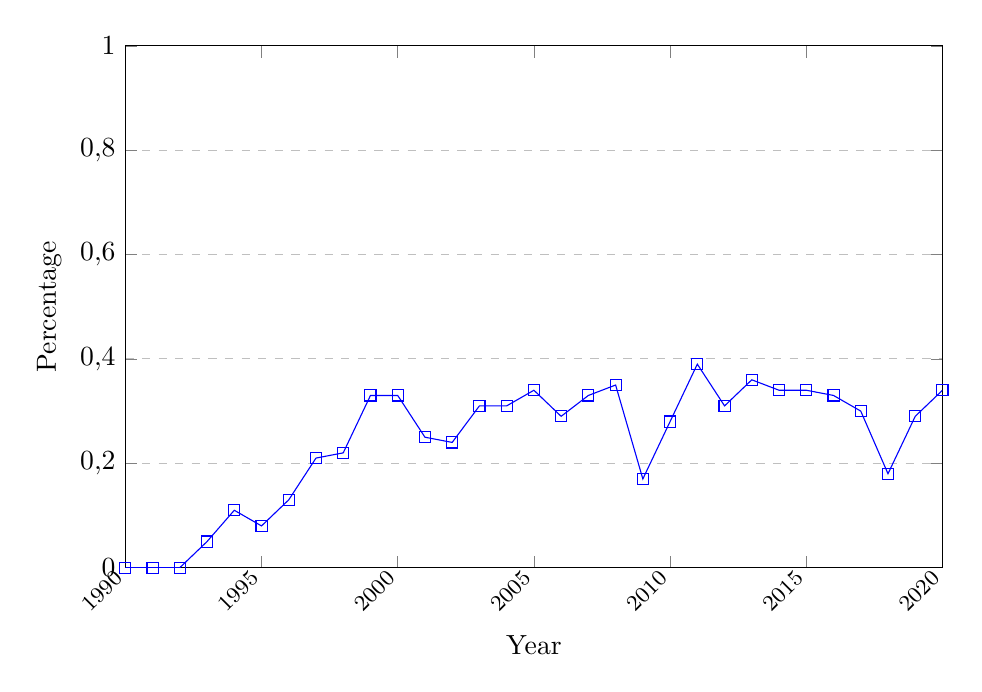
\begin{tikzpicture}
\begin{axis}[
     /pgf/number format/.cd,
     use comma,
    1000 sep={},
    width=8.5cm, height=6cm, 
    xlabel={Year},
    ylabel={Percentage},
    scale=1.5,
    xmin=1990, xmax=2020,
    ymin=0, ymax=1,
    x tick label style={font=\footnotesize,rotate=45, anchor=east},
    legend pos=north west,
    ymajorgrids=true,
    grid style=dashed,
]
\addplot[
    color=blue,
    mark=square,
    ]
    coordinates {
(1990,0.0)
(1991,0.0)
(1992,0.0)
(1993,0.05)
(1994,0.11)
(1995,0.08)
(1996,0.13)
(1997,0.21)
(1998,0.22)
(1999,0.33)
(2000,0.33)
(2001,0.25)
(2002,0.24)
(2003,0.31)
(2004,0.31)
(2005,0.34)
(2006,0.29)
(2007,0.33)
(2008,0.35)
(2009,0.17)
(2010,0.28)
(2011,0.39)
(2012,0.31)
(2013,0.36)
(2014,0.34)
(2015,0.34)
(2016,0.33)
(2017,0.3)
(2018,0.18)
(2019,0.29)
(2020,0.34)

    };
  
    
\end{axis}
\end{tikzpicture}
\caption{Top 100 email addresses belonging to authors of RFCs}
\end{figure}

All graphs regarding linking email adresses of authors to messages in the email archives, start at the year 1992. This is caused by the lack of data. RFCs in the datatracker do not contain the addresses of authors prior to said year, making it impossible to link authors of said RFCs to their messages. Those messages may very well be in the archives, there is simply no way of knowing given the current implementation.\\  
Data in the following years is also sparse, which is likely the cause of the large variation seen in those years.\\


The data shows a quite promising trend, given the relatively small amount of authors, as compared to the rest of all posters, they still take up around 25 to 40 positions in the top 100 posters. This means that authors are indeed very active participants that are responsible for a significant amount of messages sent each year. It also means that the IETF is more than just a forum that authors use to discuss among themselves. They definitely are some of the most active users, but definitely not the only ones.


\begin{figure}[H]
\hspace*{-0.5cm}
\centering
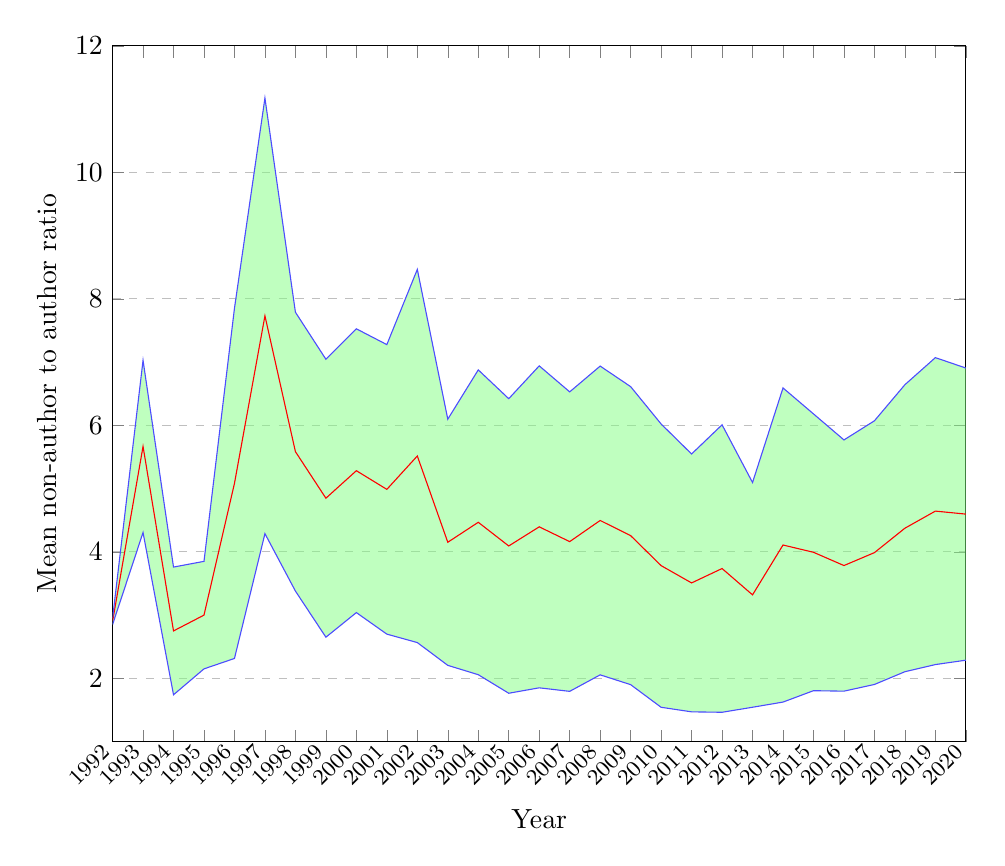
\begin{tikzpicture}
\begin{axis}[
     /pgf/number format/.cd,
     use comma,
    1000 sep={},
    width=7cm, height=6cm, 
    xlabel={Year},
    ylabel={Mean non-author to author ratio },
    scale=2,
    xmin=1992, xmax=2020,
    ymin=1, ymax=12,
    xtick={1990,1991,1992,1993 ,1994,1995,1996,1997,1998,1999,2000,2001,2002,2003,2004,2005,2006,2007,2008,2009,2010,2011,2012,2013,2014,2015,2016,2017,2018,2019,2020},
    x tick label style={font=\footnotesize,rotate=45, anchor=east},
    legend pos=north west,
    ymajorgrids=true,
    grid style=dashed,
]
\addplot[color=red] coordinates {
(1992,2.9)
(1993,5.666666666666667)
(1994,2.75)
(1995,3.0)
(1996,5.082539682539683)
(1997,7.731084656084657)
(1998,5.584269097905461)
(1999,4.847924164189224)
(2000,5.282861699703805)
(2001,4.987842819573588)
(2002,5.515574278797419)
(2003,4.15163179043179)
(2004,4.467436656910341)
(2005,4.093001624968838)
(2006,4.395424868978587)
(2007,4.161878249955173)
(2008,4.496229222973408)
(2009,4.256337134074361)
(2010,3.7821703235936814)
(2011,3.508875276169797)
(2012,3.7362788005645147)
(2013,3.319923549643829)
(2014,4.108154416672369)
(2015,3.9930329057915266)
(2016,3.7835424345769173)
(2017,3.987767407323859)
(2018,4.373871413367211)
(2019,4.6442471791029485)
(2020,4.596609779109779)
};


\addplot[name path=us_top,color=blue!70] coordinates {
(1992,2.95)
(1993,7.02749430154621)
(1994,3.7595034532988096)
(1995,3.8498365855987977)
(1996,7.850446861924698)
(1997,11.174428434557287)
(1998,7.78839150411482)
(1999,7.045049134242678)
(2000,7.5259473861447646)
(2001,7.276372804332928)
(2002,8.465242192560984)
(2003,6.097548670659342)
(2004,6.876893126556595)
(2005,6.421334010500809)
(2006,6.940366467894085)
(2007,6.529110819382916)
(2008,6.936747148674684)
(2009,6.612047816416602)
(2010,6.021448951319898)
(2011,5.54714990632174)
(2012,6.0085293463935425)
(2013,5.096474252362692)
(2014,6.591206656942355)
(2015,6.1809184669878405)
(2016,5.769328567027841)
(2017,6.07187202465043)
(2018,6.642577891067278)
(2019,7.070453330559957)
(2020,6.905710891173541)
};


\addplot[name path=us_down,color=blue!70] coordinates {
(1992,2.8499999999999996)
(1993,4.305839031787124)
(1994,1.7404965467011901)
(1995,2.1501634144012023)
(1996,2.3146325031546686)
(1997,4.287740877612027)
(1998,3.3801466916961034)
(1999,2.6507991941357694)
(2000,3.039776013262845)
(2001,2.6993128348142488)
(2002,2.5659063650338543)
(2003,2.2057149102042386)
(2004,2.0579801872640875)
(2005,1.7646692394368664)
(2006,1.8504832700630889)
(2007,1.7946456805274296)
(2008,2.0557112972721328)
(2009,1.9006264517321196)
(2010,1.542891695867465)
(2011,1.470600646017854)
(2012,1.4640282547354868)
(2013,1.5433728469249655)
(2014,1.6251021764023834)
(2015,1.8051473445952126)
(2016,1.7977563021259937)
(2017,1.9036627899972873)
(2018,2.1051649356671445)
(2019,2.2180410276459406)
(2020,2.287508667046018)
};






\addplot[green!50,fill opacity=0.5] fill between[of=us_top and us_down];
  
    
\end{axis}
\end{tikzpicture}
\caption{The mean of the ratio of non-authors to authors in the top 20 posters in a working group. The shaded area indicates the standard deviation.}
\end{figure}




\begin{figure}[H]
\hspace*{-0.5cm}
\centering
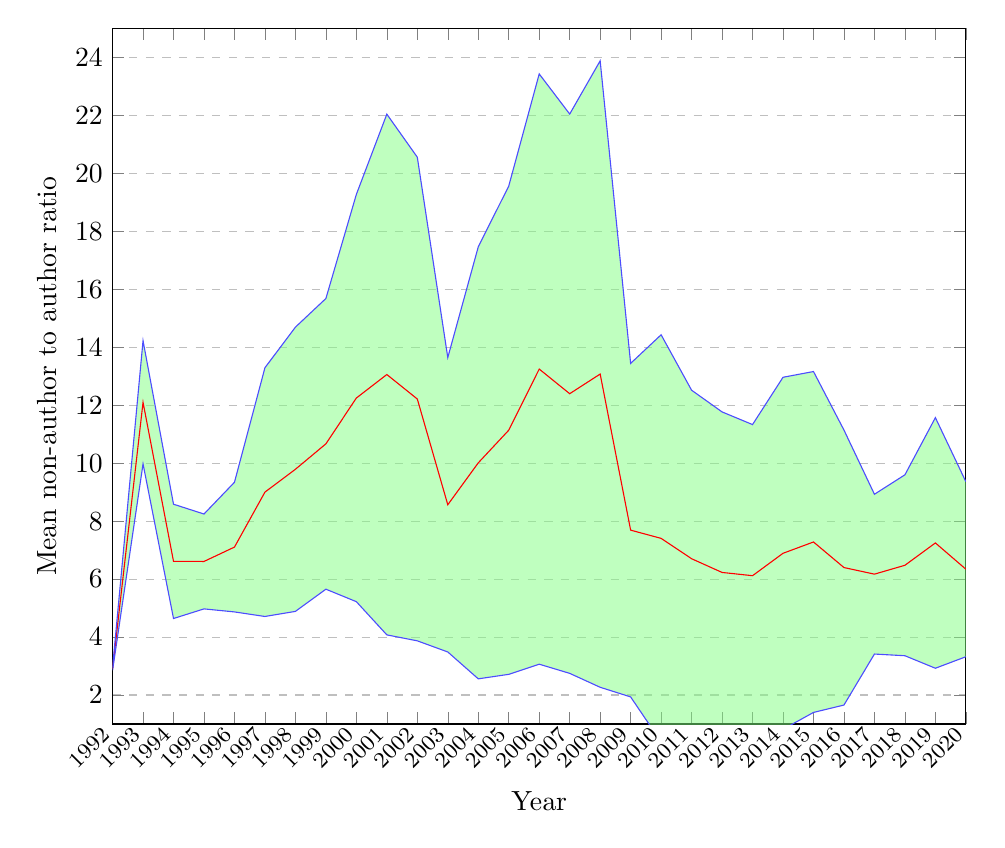
\begin{tikzpicture}
\begin{axis}[
     /pgf/number format/.cd,
     use comma,
    1000 sep={},
    width=7cm, height=6cm, 
    xlabel={Year},
    ylabel={Mean non-author to author ratio},
    scale=2,
    xmin=1992, xmax=2020,
    ymin=1, ymax=25,
    xtick={1990,1991,1992,1993 ,1994,1995,1996,1997,1998,1999,2000,2001,2002,2003,2004,2005,2006,2007,2008,2009,2010,2011,2012,2013,2014,2015,2016,2017,2018,2019,2020},
    x tick label style={font=\footnotesize,rotate=45, anchor=east},
    legend pos=north west,
    ymajorgrids=true,
    grid style=dashed,
]

\addplot[color=red] coordinates {
(1992,2.9)
(1993,12.097222222222221)
(1994,6.611111111111111)
(1995,6.607954545454546)
(1996,7.1033333333333335)
(1997,8.999693362193362)
(1998,9.78769077961352)
(1999,10.664359201166064)
(2000,12.244593284056126)
(2001,13.055564425001576)
(2002,12.210450008935537)
(2003,8.563354049280607)
(2004,10.008821808072192)
(2005,11.134915248683626)
(2006,13.24380653561535)
(2007,12.393755244587457)
(2008,13.071598186554604)
(2009,7.687837407471444)
(2010,7.40395625629824)
(2011,6.701907362962169)
(2012,6.228895617775256)
(2013,6.116631190612625)
(2014,6.889446218907785)
(2015,7.279464559055016)
(2016,6.397618233358824)
(2017,6.1701479418746965)
(2018,6.476066768336391)
(2019,7.246304747528565)
(2020,6.3408490306133505)
};


\addplot[name path=us_top,color=blue!70] coordinates {
(1992,2.95)
(1993,14.222108747878021)
(1994,8.582550705436555)
(1995,8.244029626546816)
(1996,9.339552861415891)
(1997,13.289592417850027)
(1998,14.68934910810076)
(1999,15.677528468035145)
(2000,19.269090381135314)
(2001,22.03572505912154)
(2002,20.551150516113015)
(2003,13.641024972940462)
(2004,17.458515460018745)
(2005,19.55566977876152)
(2006,23.423648180945193)
(2007,22.03938950314682)
(2008,23.875424362386084)
(2009,13.440274033428647)
(2010,14.426233144897193)
(2011,12.514855849559396)
(2012,11.765868044614805)
(2013,11.329036622375618)
(2014,12.960319196346916)
(2015,13.158558429103222)
(2016,11.139942441683917)
(2017,8.925841597214218)
(2018,9.59623914170881)
(2019,11.568041320675276)
(2020,9.360110616896266)
};


\addplot[name path=us_down,color=blue!70] coordinates {
(1992,2.8499999999999996)
(1993,9.972335696566422)
(1994,4.639671516785666)
(1995,4.971879464362277)
(1996,4.867113805250776)
(1997,4.709794306536697)
(1998,4.886032451126279)
(1999,5.6511899342969825)
(2000,5.2200961869769404)
(2001,4.0754037908816105)
(2002,3.869749501758058)
(2003,3.485683125620751)
(2004,2.55912815612564)
(2005,2.714160718605733)
(2006,3.0639648902855097)
(2007,2.748120986028095)
(2008,2.2677720107231227)
(2009,1.9354007815142404)
(2010,0.3816793676992889)
(2011,0.888958876364943)
(2012,0.6919231909357073)
(2013,0.9042257588496332)
(2014,0.8185732414686546)
(2015,1.4003706890068113)
(2016,1.6552940250337302)
(2017,3.4144542865351752)
(2018,3.355894394963972)
(2019,2.9245681743818537)
(2020,3.321587444330435)
};




\addplot[green!50,fill opacity=0.5] fill between[of=us_top and us_down];
  
    
\end{axis}
\end{tikzpicture}
\caption{The mean of the ratio of non-authors to authors in the top 100 posters in a working group.  The shaded area indicates the standard deviation.}
\end{figure}

Overall figures 8.4 and 8.5 tell the same story. Authors are active participants in a larger discussion, and while the exact amount of authors has varied somewhat through the years, they have always been some of the most active users.
Reaching its peak around 2012-2013, and reaching the lowest point at around 2018, the amount of authors has been sharply increasing since. 



\subsection{Search strategy}

Knowing this opens up for new possibilities when it comes to conversation tracking. One major “flaw” of the method previously described in this chapter is its reliance on keywords. An RFC does not get its number until it is published. This means that using for example “RFC 822” as a query term, will return conversations mentioning said RFC, which again means that they must have occurred after its publication. While this in itself can be useful, it does not provide anything useful in regards to how said RFC came to be.


With the now added option of investigating specific authors one can look for the conversation an author of any given RFC had before the RFC was published. But how does one do this? The current implementation, as said queries the “Subject” and “Content” fields, then uses the results returned by Solr to calculate conversation threads. This however, can be quite easily changed; as the current implementation uses a set of nodes to calculate threads, simply providing a more sutiable set of nodes will result in better results. But in that case, what kind of queries are likely to give the best results?
A good starting point would be to query a specific time frame before an RFC was published. The exact size of the timeframe, will of course vary from RFC to RFC, but 1 year is expected to at the very least be a good starting point. The next improvement would be to focus on the authors of the RFC one is trying to investigate. The underlying assumption here is that the author will generally be the “driving force” behind a conversation, and if a suitable value for the thread tracking program's lookahead is chosen, the responses and replies from other participants are likely to be included in the thread.
Finally, the two fields that were originally used are still relevant, as they tell something about the nature of a conversation. What to query for in these fields is up for debate, generally speaking, querying for the number of an RFC will not yield good results. Keywords relating to the desired topic are expected to be much more effective. 
For example,if we wish to look for threads that may have led to the creation of RFC 2822 \cite{RFC2822}, querying RFC 2822 \cite{RFC2822}, will not work. However, querying for a keyword such as “email standard” or “message format” is expected to result in much more relevant threads when combined with the two previously discussed query options.




\chapter{Conclusion}

To sum up the entire project, the mail archives have been parsed and transformed into a searchable state in an advanced text search database. The parser used for this purpose is not limited to parsing the IETF email archives; any archives in the mbox format can be parsed using this software.
The messages in the email archives have been linked together using the available data to graphs representing a relation between messages. Said graphs have been used in an attempt to track down desired conversation threads that may contain information regarding the creation of specific RFCs. While an answer has not yet been found and there is still much work to do, the groundwork has been laid for further research, should anyone wish to continue this work. Here are some pointers as to how to improve the project in various ways.

\subsubsection{Spam detection} 
The email archives are unfortunately full of messages that do not bear any meaningful or useful information in regard to the goals of this project. Many of these are automated messages trying to sell various things such as medication, or cheap cloned products. Removing these from the database would greatly improve the quality of the data within. As we saw earlier, looking for highly contested email addresses is a good way to start.

\subsubsection{Machine learning}
As the current thread tracker relies on the results passed on by Solr, figuring out a good search strategy, and using the results returned by using said strategy, may be a good way to start implementing machine learning in an attempt to retrieve better results. The results passed from asol are after all calculated with cosine similarity (as depending on the configuration of a given field), which is often used as a baseline that a given machine learning algorithm needs to beat.  

\subsubsection{Improving the parsing process}
The parsing process will always be a highly important stepping stone for this project. As we saw in chapter 7, a lot of messages have flaws, and are missing vital data in their fields. Remedying this problem is surely to improve the result and conversation that can be retrieved from the database.

\subsubsection{Restoring and parsing the attachments}
Attachments carried by messages were left out of this project, mainly due to time constraints. They are a whole new source of untapped information that is ready to be restored into its original form, and parsed.

\subsubsection{A better idea of a person}
Being able to ascribe the messages sent by several email addresses to a single person can be very valuable. We already saw a fragment of it when working on tracking the work of authors specifically. This is however not a trivial task, and probably goes hand in hand with spam detection, as removing the work of automated processes, such as notification messages, or simply spam. Trying to sell some unspecified product at allegedly very attractive prices will increase the probability that a given message was in fact sent by an actual human being.
How exactly this is done is not yet clear, however, organizing all email addresses in the database into categories could be a first step.  For example, looking for patterns in email addresses of automated messages.
This is also an instance where machine learning could prove to be very useful, as it has already been, and is being used to identify individuals matched on many aspects of their behaviour.
 

\subsubsection{Establishing linear time}
A major issue with both the graphs, nodes, and conversation tracking is the fragile concept of time, at least as it seems to be in the current database. A way to properly order the emails sequentially, and giving proper, or at least better estimation of when they were actually sent, would likely help to improve the results. Establishing, enforcing, and resolving family tree rule violations is also expected to be highly beneficial, as once we know that the child of a parent is guaranteed to be younger, they can be ordered appropriately.

These are just some of the suggestions from the author of this thesis. There probably are many other things that could be changed and altered in order to improve the overall quality of the project.







\chapter{Appendix}

\section{Known issues and fixes}

\textbf{Issue 1:}\\

Some of the strings returned by Solr from the address field are not immediately searchable due to how Solr manages special characters and spaces. 
This is a problem as it is these strings or “tokens” that are returned by the facet function, and are often used to calculate statistics for this project.

Example:\\
"Dose <zeroconf-archive"@lists.ietf.org\\
"Dose <kink-archive"@megatron.ietf.org\\
"Dose <dnsext-archive"@ietf.org\\
"greetingll-yours.net"@129-79-115-30.dhcp-bl.indiana.edu\\
"greetingll-yours.net"@mail.difusoradigital.com.ar\\
".com"@truemail.co.th\\
".org"@afa.org.ar\\
"Prof. Jesus Dolphin"@core3.amsl.com\\

To remedy this a method was created to restore these strings to a form accepted by Solr.
This method is called “fix\_adr(inn)”, takes a string as input, and outputs a more Solr friendly version.  
This method should only be used if a query with a non processed string fails.\\

\noindent
\textbf{Issue 2:}\\\\
Similar to issue 1 there are some characters that are not accepted by Solr.
This also depends on where in the string these characters are found.
Characters that cannot be at the beginning of a string are as follows:\\

+,-,~,!\\



Characters that are not allowed in any position in the string are as follows:\\

“,/,[,],\{,\},\^,:\\

The method mentioned in issue 1 has been expanded to also handle these characters, and should be used in the same circumstances as issue 1. 


\section{List of Solr cores}

\subsubsection{author}

This "author" core contains a set of authors, with their names, and email addresses.


\begin{center}
 \begin{tabular}{||c | c||} 
 \hline
 \textit{Field name} & \textit{Tokenizer} \\ [1ex] 
 \hline\hline


name & solr.KeywordTokenizerFactory\\

\hline

address & solr.KeywordTokenizerFactory\\

\hline


\end{tabular}
\end{center}

\subsubsection{rfc}
This “rfc” core contains information about RFCs, including their authors, time of publication, id and title.

\begin{center}
 \begin{tabular}{||c | c||} 
 \hline
 \textit{Field name} & \textit{Tokenizer} \\ [1ex] 
 \hline\hline


date & No tokenizer\\

\hline


number & No tokenizer\\

\hline


author & solr.KeywordTokenizerFactory\\

\hline



title & solr.StandardTokenizerFactory\\

\hline


\end{tabular}
\end{center}


\subsubsection{graphs}

This core is used to store the conversation graphs.

\begin{center}
 \begin{tabular}{||c c||} 
 \hline
 \textit{Field} & \textit{Tokenizer} \\ [1ex] 
 \hline\hline

graph-id & No tokenizer\\

\hline

nodes & solr.KeywordTokenizerFactory\\

\hline

\end{tabular}
\end{center}


\subsubsection{nodes}


This core contains the nodes of the conversation graphs. Each node has information regarding iself, as well as its immediate neighbours, that being its parents and children. 


\begin{center}
 \begin{tabular}{||c c||} 
 \hline
 \textit{Field} & \textit{Tokenizer} \\ [1ex] 
 \hline\hline


node-id & solr.KeywordTokenizerFactory\\

\hline

graph-id & No tokenizer\\

\hline

parent & solr.KeywordTokenizerFactory\\

\hline

child & solr.KeywordTokenizerFactory\\

\hline



\end{tabular}
\end{center}




\subsubsection{ietf-archive-final-v2}

This is the main core, it is this core that contains the parsed email archives, and it is this core that was used for calculating statistics, tracking conversations and many other things.

\begin{center}
 \begin{tabular}{||c | c||} 
 \hline
 \textit{Field} & \textit{Tokenizer} \\ [1ex] 
 \hline\hline
 Date & No tokenizer\\ 

 \hline
 Date-raw &  solr.KeywordTokenizerFactory\\

\hline
Timezone & solr.KeywordTokenizerFactory\\

\hline 
From & solr.StandardTokenizerFactory\\

\hline
From-name & solr.KeywordTokenizerFactory\\

\hline
From-address & solr.UAX29URLEmailTokenizerFactory\\

\hline 
Sender & solr.StandardTokenizerFactory\\

\hline
Sender-name & solr.KeywordTokenizerFactory\\

\hline
Sender-address & solr.UAX29URLEmailTokenizerFactory\\

\hline 
Reply-to & solr.StandardTokenizerFactory\\

\hline
Reply-to-name & solr.KeywordTokenizerFactory\\

\hline
Reply-to-address & solr.UAX29URLEmailTokenizerFactory\\

\hline 
To & solr.StandardTokenizerFactory\\

\hline
To-name & solr.KeywordTokenizerFactory\\

\hline
To-address & solr.UAX29URLEmailTokenizerFactory\\

\hline 
Cc & solr.StandardTokenizerFactory\\

\hline
Cc-name & solr.KeywordTokenizerFactory\\

\hline
Cc-address & solr.UAX29URLEmailTokenizerFactory\\

\hline 
In-Reply-To & solr.StandardTokenizerFactory\\

\hline
In-Reply-To-name & solr.KeywordTokenizerFactory\\

\hline
In-Reply-To-address & solr.UAX29URLEmailTokenizerFactory\\

\hline 
Message-ID &  solr.KeywordTokenizerFactory\\

\hline 
 References &  solr.KeywordTokenizerFactory \\

\hline 
Comments &  solr.StandardTokenizerFactory \\

\hline 
Subject &  solr.StandardTokenizerFactory \\

\hline 
Content &  solr.StandardTokenizerFactory \\

\hline 
Mailing-list & solr.KeywordTokenizerFactory \\

\hline
File-location &  solr.StandardTokenizerFactory \\
\hline
\end{tabular}
\end{center}








\printbibliography










\end{document}